% Options for packages loaded elsewhere
\PassOptionsToPackage{unicode}{hyperref}
\PassOptionsToPackage{hyphens}{url}
%
\documentclass[
]{book}
\title{Engaging with MIDFIELD Data}
\author{Susan Lord, Matthew Ohland, Marisa Orr, Richard Layton, and Russell Long}
\date{2021-07-26}

\usepackage{amsmath,amssymb}
\usepackage{lmodern}
\usepackage{iftex}
\ifPDFTeX
  \usepackage[T1]{fontenc}
  \usepackage[utf8]{inputenc}
  \usepackage{textcomp} % provide euro and other symbols
\else % if luatex or xetex
  \usepackage{unicode-math}
  \defaultfontfeatures{Scale=MatchLowercase}
  \defaultfontfeatures[\rmfamily]{Ligatures=TeX,Scale=1}
\fi
% Use upquote if available, for straight quotes in verbatim environments
\IfFileExists{upquote.sty}{\usepackage{upquote}}{}
\IfFileExists{microtype.sty}{% use microtype if available
  \usepackage[]{microtype}
  \UseMicrotypeSet[protrusion]{basicmath} % disable protrusion for tt fonts
}{}
\makeatletter
\@ifundefined{KOMAClassName}{% if non-KOMA class
  \IfFileExists{parskip.sty}{%
    \usepackage{parskip}
  }{% else
    \setlength{\parindent}{0pt}
    \setlength{\parskip}{6pt plus 2pt minus 1pt}}
}{% if KOMA class
  \KOMAoptions{parskip=half}}
\makeatother
\usepackage{xcolor}
\IfFileExists{xurl.sty}{\usepackage{xurl}}{} % add URL line breaks if available
\IfFileExists{bookmark.sty}{\usepackage{bookmark}}{\usepackage{hyperref}}
\hypersetup{
  pdftitle={Engaging with MIDFIELD Data},
  pdfauthor={Susan Lord, Matthew Ohland, Marisa Orr, Richard Layton, and Russell Long},
  hidelinks,
  pdfcreator={LaTeX via pandoc}}
\urlstyle{same} % disable monospaced font for URLs
\usepackage{color}
\usepackage{fancyvrb}
\newcommand{\VerbBar}{|}
\newcommand{\VERB}{\Verb[commandchars=\\\{\}]}
\DefineVerbatimEnvironment{Highlighting}{Verbatim}{commandchars=\\\{\}}
% Add ',fontsize=\small' for more characters per line
\usepackage{framed}
\definecolor{shadecolor}{RGB}{248,248,248}
\newenvironment{Shaded}{\begin{snugshade}}{\end{snugshade}}
\newcommand{\AlertTok}[1]{\textcolor[rgb]{0.94,0.16,0.16}{#1}}
\newcommand{\AnnotationTok}[1]{\textcolor[rgb]{0.56,0.35,0.01}{\textbf{\textit{#1}}}}
\newcommand{\AttributeTok}[1]{\textcolor[rgb]{0.77,0.63,0.00}{#1}}
\newcommand{\BaseNTok}[1]{\textcolor[rgb]{0.00,0.00,0.81}{#1}}
\newcommand{\BuiltInTok}[1]{#1}
\newcommand{\CharTok}[1]{\textcolor[rgb]{0.31,0.60,0.02}{#1}}
\newcommand{\CommentTok}[1]{\textcolor[rgb]{0.56,0.35,0.01}{\textit{#1}}}
\newcommand{\CommentVarTok}[1]{\textcolor[rgb]{0.56,0.35,0.01}{\textbf{\textit{#1}}}}
\newcommand{\ConstantTok}[1]{\textcolor[rgb]{0.00,0.00,0.00}{#1}}
\newcommand{\ControlFlowTok}[1]{\textcolor[rgb]{0.13,0.29,0.53}{\textbf{#1}}}
\newcommand{\DataTypeTok}[1]{\textcolor[rgb]{0.13,0.29,0.53}{#1}}
\newcommand{\DecValTok}[1]{\textcolor[rgb]{0.00,0.00,0.81}{#1}}
\newcommand{\DocumentationTok}[1]{\textcolor[rgb]{0.56,0.35,0.01}{\textbf{\textit{#1}}}}
\newcommand{\ErrorTok}[1]{\textcolor[rgb]{0.64,0.00,0.00}{\textbf{#1}}}
\newcommand{\ExtensionTok}[1]{#1}
\newcommand{\FloatTok}[1]{\textcolor[rgb]{0.00,0.00,0.81}{#1}}
\newcommand{\FunctionTok}[1]{\textcolor[rgb]{0.00,0.00,0.00}{#1}}
\newcommand{\ImportTok}[1]{#1}
\newcommand{\InformationTok}[1]{\textcolor[rgb]{0.56,0.35,0.01}{\textbf{\textit{#1}}}}
\newcommand{\KeywordTok}[1]{\textcolor[rgb]{0.13,0.29,0.53}{\textbf{#1}}}
\newcommand{\NormalTok}[1]{#1}
\newcommand{\OperatorTok}[1]{\textcolor[rgb]{0.81,0.36,0.00}{\textbf{#1}}}
\newcommand{\OtherTok}[1]{\textcolor[rgb]{0.56,0.35,0.01}{#1}}
\newcommand{\PreprocessorTok}[1]{\textcolor[rgb]{0.56,0.35,0.01}{\textit{#1}}}
\newcommand{\RegionMarkerTok}[1]{#1}
\newcommand{\SpecialCharTok}[1]{\textcolor[rgb]{0.00,0.00,0.00}{#1}}
\newcommand{\SpecialStringTok}[1]{\textcolor[rgb]{0.31,0.60,0.02}{#1}}
\newcommand{\StringTok}[1]{\textcolor[rgb]{0.31,0.60,0.02}{#1}}
\newcommand{\VariableTok}[1]{\textcolor[rgb]{0.00,0.00,0.00}{#1}}
\newcommand{\VerbatimStringTok}[1]{\textcolor[rgb]{0.31,0.60,0.02}{#1}}
\newcommand{\WarningTok}[1]{\textcolor[rgb]{0.56,0.35,0.01}{\textbf{\textit{#1}}}}
\usepackage{longtable,booktabs,array}
\usepackage{calc} % for calculating minipage widths
% Correct order of tables after \paragraph or \subparagraph
\usepackage{etoolbox}
\makeatletter
\patchcmd\longtable{\par}{\if@noskipsec\mbox{}\fi\par}{}{}
\makeatother
% Allow footnotes in longtable head/foot
\IfFileExists{footnotehyper.sty}{\usepackage{footnotehyper}}{\usepackage{footnote}}
\makesavenoteenv{longtable}
\usepackage{graphicx}
\makeatletter
\def\maxwidth{\ifdim\Gin@nat@width>\linewidth\linewidth\else\Gin@nat@width\fi}
\def\maxheight{\ifdim\Gin@nat@height>\textheight\textheight\else\Gin@nat@height\fi}
\makeatother
% Scale images if necessary, so that they will not overflow the page
% margins by default, and it is still possible to overwrite the defaults
% using explicit options in \includegraphics[width, height, ...]{}
\setkeys{Gin}{width=\maxwidth,height=\maxheight,keepaspectratio}
% Set default figure placement to htbp
\makeatletter
\def\fps@figure{htbp}
\makeatother
\setlength{\emergencystretch}{3em} % prevent overfull lines
\providecommand{\tightlist}{%
  \setlength{\itemsep}{0pt}\setlength{\parskip}{0pt}}
\setcounter{secnumdepth}{5}
\usepackage{booktabs}
\usepackage{amsthm}
\makeatletter
\def\thm@space@setup{%
  \thm@preskip=8pt plus 2pt minus 4pt
  \thm@postskip=\thm@preskip
}
\makeatother
\ifLuaTeX
  \usepackage{selnolig}  % disable illegal ligatures
\fi
\usepackage[]{natbib}
\bibliographystyle{plainnat}

\begin{document}
\maketitle

{
\setcounter{tocdepth}{1}
\tableofcontents
}
\hypertarget{introduction}{%
\chapter{Introduction}\label{introduction}}

\hypertarget{objectives}{%
\section{Objectives}\label{objectives}}

\href{https://engineering.purdue.edu/MIDFIELD}{\textbf{MIDFIELD}} contains individual Student Unit Record (SUR) data for 1.7M students at 33 US institutions (as of June 2021). MIDFIELD is large enough to permit grouping and summarizing by multiple characteristics, enabling researchers to examine student characteristics (race/ethnicity, sex, prior achievement) and curricular pathways (including coursework and major) by institution and over time.

The goal of this workshop is to engage ASEE members with MIDFIELD data, in part using two R packages: \href{https://midfieldr.github.io/midfieldr/}{\textbf{midfieldr}} to provide tools for working with SURs and \href{https://midfieldr.github.io/midfielddata/}{\textbf{midfielddata}} to provide practice data.

By the end of the workshop, participants should be able to:

\begin{itemize}
\tightlist
\item
  Describe key variables in MIDFIELD data tables
\item
  Explore and tell a story from MIDFIELD data
\item
  Begin using R, midfieldr, and midfielddata\\
\item
  Explain key features of effective data displays
\end{itemize}

\hypertarget{description}{%
\section{Description}\label{description}}

The robustness of the MIDFIELD data allows us to emphasize an intersectional approach to the study of student records, permitting multiple categories of inequity such as race/ethnicity and sex to be considered simultaneously.

To introduce beginners to R, participants work through a self-paced tutorial covering basic elements of the R computing language and environment. To introduce midfieldr and using it to work with student record data, participants work through software tutorials that explore the SUR data and develop a persistence metric case study.

For more experienced R users or anyone working at a faster pace, we offer a series of self-paced tutorials that introduce key features of midfieldr and how they are applied to compute persistence metrics and graph results.

We also discuss the merits of the multiway graph design that is recommended for displaying results of this type. The agenda includes an interactive session to demonstrate contemporary principles of effective data display.

\hypertarget{pre-workshop-homework}{%
\section{Pre-workshop homework}\label{pre-workshop-homework}}

To get the most out of the workshop, you should have the essential software installed and running several days before the workshop to give you time to contact us with questions if anything goes amiss.

\protect\hyperlink{install-everything}{Install everything} describes the homework.

\hypertarget{agenda}{%
\section{Agenda}\label{agenda}}

Our three hours are organized approximately as shown.

\begin{tabular}{ll}
\toprule
Min & Topic\\
\midrule
15 & Introduction\\
35 & Exploring the data structure\\
35 & Working with R\\
15 & Break\\
20 & Designing effective displays\\
\addlinespace
50 & Working with R (continued)\\
10 & Next steps \& assessing the workshop\\
\bottomrule
\end{tabular}

\hypertarget{facilitators}{%
\section{Facilitators}\label{facilitators}}

\begin{description}
\item[Susan Lord]
Director of the MIDFIELD Institute and Professor and Chair of Integrated Engineering at the University of San Diego. She is a Fellow of the IEEE and the ASEE. Dr.~Lord has considerable experience facilitating workshops including the National Effective Teaching Institute (NETI) and special sessions at FIE. (\href{mailto:slord@sandiego.edu}{\nolinkurl{slord@sandiego.edu}})
\item[Matthew Ohland]
MIDFIELD Director and Principal Investigator. He is Professor and Associate Head of Engineering Education at Purdue University and a Fellow of IEEE, ASEE, and AAAS. Dr.~Ohland has considerable experience facilitating workshops including the NETI and CATME training. (\href{mailto:ohland@purdue.edu}{\nolinkurl{ohland@purdue.edu}})
\item[Marisa Orr]
MIDFIELD Associate Director and Associate Professor in Engineering and Science Education with a joint appointment in Mechanical Engineering at Clemson University. She received the 2009 Helen Plants Award for the best nontraditional session at FIE, ``Enhancing Student Learning Using SCALE-UP Format.'' (\href{mailto:marisak@clemson.edu}{\nolinkurl{marisak@clemson.edu}})
\item[Richard Layton]
MIDFIELD Data Visualization Specialist and Professor Emeritus of Mechanical Engineering at Rose-Hulman Institute of Technology. He is the lead developer of the R packages used in this workshop. Dr.~Layton has considerable experience facilitating workshops, including FIE workshops on data visualization (2014) and midfieldr (2018). (\href{mailto:graphdoctor@gmail.com}{\nolinkurl{graphdoctor@gmail.com}})
\item[Russell Long]
MIDFIELD Managing Director and Data Steward. He developed the stratified data sample for the R packages used in this workshop. Mr.~Long is a SAS expert with over twenty years of experience in institutional research and assessment. (\href{mailto:ralong@purdue.edu}{\nolinkurl{ralong@purdue.edu}})
\end{description}

\hypertarget{licenses}{%
\section{Licenses}\label{licenses}}

The following licenses apply to the text, data, and code in these workshops. Our goal is to minimize legal encumbrances to the dissemination, sharing, use, and re-use of this work. However, the existing rights of authors whose work is cited (text, code, or data) are reserved to those authors.

\begin{itemize}
\tightlist
\item
  \href{https://creativecommons.org/licenses/by/4.0/legalcode}{CC-BY 4.0} for all text\\
\item
  \href{https://www.r-project.org/Licenses/GPL-3}{GPL-3} for all code\\
\item
  \href{https://wiki.creativecommons.org/wiki/CC0_use_for_data}{CC0} for all data
\end{itemize}

\hypertarget{acknowledgement}{%
\section{Acknowledgement}\label{acknowledgement}}

Funding provided by the National Science Foundation Grant 1545667 ``Expanding Access to and Participation in the Multiple-Institution Database for Investigating Engineering Longitudinal Development.''

\protect\hyperlink{introduction}{▲ top of page}

\hypertarget{install-everything}{%
\chapter{Install everything}\label{install-everything}}

If you are trying R for the first time, it is vital that you attempt to set up your computer with the necessary software in advance or it will be difficult to keep up.

This chapter describes all of the pre-workshop homework:

\begin{itemize}
\tightlist
\item
  \protect\hyperlink{already-installed}{Already installed?}
\item
  \protect\hyperlink{install-r-and-rstudio}{Install R and RStudio}
\item
  \protect\hyperlink{create-a-project}{Create a project}\\
\item
  \protect\hyperlink{add-some-folders}{Add some folders}
\item
  \protect\hyperlink{install-cran-packages}{Install CRAN packages}
\item
  \protect\hyperlink{install-midfield-packages}{Install MIDFIELD packages}
\end{itemize}

\hypertarget{already-installed}{%
\section{Already installed?}\label{already-installed}}

If you do not have R and RStudio installed, please skip this section and start with the next section. If you are already an R and RStudio user, this is a great time to check for updates.

\textbf{Updating RStudio}

\begin{itemize}
\tightlist
\item
  RStudio menu \emph{Help \textgreater{} Check for Updates} will tell you if you are current or not.
\item
  To update, close RStudio on your machine, download the new version from the \href{https://www.rstudio.com/products/rstudio/\#Desktop}{RStudio website}, and run the \texttt{RStudio-some-version-number.exe}. (Windows users \emph{might} have to run the executable as an administrator.)
\end{itemize}

\textbf{Update your packages}

\href{https://rstats.wtf/maintaining-r.html\#how-to-upgrade-all-out-of-date-packages}{How to upgrade all out-of-date packages} in \emph{What They Forgot to Teach You About R} by Jennifer Bryan and Jim Hester.

\textbf{Updating R}

The easiest way to update R is to simply \href{https://cloud.r-project.org/}{download the newest version}. RStudio will automatically use the latest you've installed.

Alternatively, Windows users can use the installr package:

\begin{itemize}
\tightlist
\item
  Install the installr package
\item
  If open, close R and RStudio
\item
  Navigate to your most recent \texttt{Rgui.exe} file located in your Programs directory, e.g., \texttt{C:\textbackslash{}Program\ Files\textbackslash{}R\textbackslash{}R-4.0.0\textbackslash{}bin\textbackslash{}x64\textbackslash{}Rgui.exe}\\
\item
  Right-click on \texttt{Rgui.exe} and run as administrator
\item
  In the R GUI window that appears, run the commands
\end{itemize}

\begin{Shaded}
\begin{Highlighting}[]
    \CommentTok{\# Windows users only}
    \FunctionTok{library}\NormalTok{(}\StringTok{"installr"}\NormalTok{)}
    \FunctionTok{updateR}\NormalTok{()}
\end{Highlighting}
\end{Shaded}

\textbf{Updating your R library}

\href{https://rstats.wtf/maintaining-r.html\#how-to-transfer-your-library-when-updating-r}{How to transfer your library when updating R} also by Bryan and Hester. Requires the fs package.

\textbf{Once your updates are complete}

Skip the next section and continue the homework with

\begin{itemize}
\tightlist
\item
  \protect\hyperlink{create-a-project}{Create a project}\\
\item
  \protect\hyperlink{add-some-folders}{Add some folders}
\item
  \protect\hyperlink{install-cran-packages}{Install CRAN packages}
\item
  \protect\hyperlink{install-midfield-packages}{Install MIDFIELD packages}
\end{itemize}

\hypertarget{install-r-and-rstudio}{%
\section{Install R and RStudio}\label{install-r-and-rstudio}}

The first steps are to install R and RStudio. Windows users may have to login as an Administrator before installing the software.

\begin{itemize}
\tightlist
\item
  \href{https://cloud.r-project.org}{Install R} for your operating system\\
\item
  \href{https://www.rstudio.com/products/rstudio/download/\#download}{Install RStudio}, a user interface for R
\end{itemize}

Once the installation is complete, you can take a 2-minute tour of the RStudio interface.

\begin{itemize}
\tightlist
\item
  \href{https://www.youtube.com/embed/kfcX5DEMAp4?start=57\&end=152}{Let's start (00:57--02:32)} by R Ladies Sydney \citep{RLadiesSydney:2018:Lesson1}
\end{itemize}

The same video includes a longer (7 minute) tour of the four quadrants (panes) in RStudio if you are interested.

\begin{itemize}
\tightlist
\item
  \href{https://www.youtube.com/embed/kfcX5DEMAp4?start=441\&end=880}{The RStudio quadrants (07:21--14:40)} by R Ladies Sydney \citep{RLadiesSydney:2018:Lesson1}
\end{itemize}

\hypertarget{create-a-project}{%
\section{Create a project}\label{create-a-project}}

To begin any project, we create an RStudio \emph{Project} file and directory. You can recognize an R project file by its \emph{.Rproj} suffix.

If you prefer your instructions with commentary,

\begin{itemize}
\tightlist
\item
  \href{https://www.youtube.com/embed/kfcX5DEMAp4?start=154\&end=290}{Start with a Project (02:34--04:50)} by R Ladies Sydney \citep{RLadiesSydney:2018:Lesson1}
\end{itemize}

If you prefer basic written instructions,

\begin{itemize}
\tightlist
\item
  RStudio, \emph{File \textgreater{} New Project\ldots{} \textgreater{} New Directory \textgreater{} New Project}
\item
  Or, click the \emph{New Project} button in the Console ribbon,
\end{itemize}

In the dialog box that appears,

\begin{itemize}
\tightlist
\item
  Type the workshop name as the directory name, for example, \texttt{workshop}, or if you like more detail, \texttt{midfield-workshop-asee-2021}\\
\item
  Use the browse button to select a location on your computer to create the project folder\\
\item
  Click the \emph{Create Project} button
\end{itemize}

Whenever you work with the workshop materials, launch the \texttt{workshop.Rproj} file (using the name you actually used) to start the session.

\hypertarget{add-some-folders}{%
\section{Add some folders}\label{add-some-folders}}

While file organization is a matter of personal preference, we ask that you use the directory structure shown here for your work in the workshop. Assuming we called our project \texttt{workshop}, the minimal directory structure has three folders in it plus the \texttt{.Rproj} file at the top level.

\begin{Shaded}
\begin{Highlighting}[]
\NormalTok{\textbackslash{}workshop}
\NormalTok{    \textbackslash{}data}
\NormalTok{    \textbackslash{}results}
\NormalTok{    \textbackslash{}scripts}
\NormalTok{    workshop.Rproj}
\end{Highlighting}
\end{Shaded}

We use the folders as follows:

\begin{itemize}
\tightlist
\item
  \texttt{data} data files
\item
  \texttt{results} finished graphs and tabulated data formatted for display\\
\item
  \texttt{scripts} R scripts that operate on data to produce results
\end{itemize}

To create folders:

\begin{itemize}
\tightlist
\item
  use your usual method of creating new folders on your machine
\item
  or you can use the \emph{New Folder} button in the Files pane
\end{itemize}

For a video guide,

\begin{itemize}
\tightlist
\item
  \href{https://www.youtube.com/embed/kfcX5DEMAp4?start=290\&end=368}{Make some folders (04:50--06:08)} by R Ladies Sydney \citep{RLadiesSydney:2018:Lesson1}
\end{itemize}

\hypertarget{install-cran-packages}{%
\section{Install CRAN packages}\label{install-cran-packages}}

The fundamental unit of shareable code in R is the \emph{package.} For the R novice, an R package is like an ``app'' for R---a collection of functions, data, and documentation for doing work in R that is easily shared with others \citep{wickham2014advanced}.

Most packages are obtained from the \href{https://cran.r-project.org/}{CRAN} website \citep{cranweb}. To install a CRAN package using RStudio:

\begin{itemize}
\tightlist
\item
  Launch RStudio
\end{itemize}

The RStudio interface has several panes. We want the \emph{Files/Plots/Packages} pane.

\begin{itemize}
\tightlist
\item
  Select the \emph{Packages} tab
\end{itemize}

Next,

\begin{itemize}
\tightlist
\item
  Click \emph{Install} on the ribbon
\item
  In the dialog box, type the name of the package. For our first package, type \texttt{data.table} to install the data.table package \citep{R-data.table}
\item
  Check the \emph{Install dependencies} box
\item
  Click the \emph{Install} button
\end{itemize}

\begin{quote}
During the installation, Windows users might get a warning message about
Rtools, something like:

\texttt{WARNING:\ Rtools\ is\ required\ to\ build\ R\ packages\ but\ is\ not\ currently\ installed.\ Please\ download\ and\ install\ the\ appropriate\ version...}.
\end{quote}

Rtools is needed for packages with C/C++/FORTRAN code from source---which does not apply to us. You may ignore the warning and carry on.

In the RStudio Console, you should see a message like this one,

\begin{Shaded}
\begin{Highlighting}[]
\NormalTok{    package }\StringTok{\textquotesingle{}data.table\textquotesingle{}}\NormalTok{ successfully unpacked and MD5 sums checked}
\end{Highlighting}
\end{Shaded}

If successful, the package will appear in the Packages pane, e.g.,

Repeat the process for the following packages

\begin{verbatim}
wrapr 
Rdpack 
checkmate
ggplot2
\end{verbatim}

Alternatively, you can install them all at once by typing in the Console:

\begin{Shaded}
\begin{Highlighting}[]
\NormalTok{packages\_we\_use }\OtherTok{\textless{}{-}} \FunctionTok{c}\NormalTok{(}\StringTok{"data.table"}\NormalTok{, }\StringTok{"wrapr"}\NormalTok{, }\StringTok{"Rdpack"}\NormalTok{, }\StringTok{"checkmate"}\NormalTok{, }\StringTok{"ggplot2"}\NormalTok{)}
\FunctionTok{install.packages}\NormalTok{(packages\_we\_use)}
\end{Highlighting}
\end{Shaded}

\hypertarget{install-midfield-packages}{%
\section{Install MIDFIELD packages}\label{install-midfield-packages}}

\hypertarget{midfieldr}{%
\subsection{midfieldr}\label{midfieldr}}

midfieldr is not yet available from \href{https://cran.r-project.org/}{CRAN}. To install the development version of midfieldr from its \texttt{drat} repository, type in the Console:

\begin{Shaded}
\begin{Highlighting}[]
\CommentTok{\# type in the RStudio Console }
\FunctionTok{install.packages}\NormalTok{(}\StringTok{"midfieldr"}\NormalTok{, }
                 \AttributeTok{repos =} \StringTok{"https://MIDFIELDR.github.io/drat/"}\NormalTok{, }
                 \AttributeTok{type =} \StringTok{"source"}\NormalTok{)}
\end{Highlighting}
\end{Shaded}

You can confirm a successful installation by running the following lines to bring up the package help page in the Help window.

\begin{Shaded}
\begin{Highlighting}[]
\CommentTok{\# type in the RStudio Console }
\FunctionTok{library}\NormalTok{(}\StringTok{"midfieldr"}\NormalTok{)}
\NormalTok{? }\StringTok{\textasciigrave{}}\AttributeTok{midfieldr{-}package}\StringTok{\textasciigrave{}}

\CommentTok{\# or, equivalently}
\FunctionTok{help}\NormalTok{(}\StringTok{"midfieldr{-}package"}\NormalTok{)}
\end{Highlighting}
\end{Shaded}

If the installation is successful, the code chunk above should produce a view of the help page as shown here.

\hypertarget{midfielddata}{%
\subsection{midfielddata}\label{midfielddata}}

Because of its size, the data package is stored in a \texttt{drat} repository instead of CRAN. Installation takes time; please be patient and wait for the Console prompt ``\textgreater{}'' to reappear.

Type (or copy and paste) the following lines in the RStudio Console.

\begin{Shaded}
\begin{Highlighting}[]
\CommentTok{\# type in the RStudio Console  }
\FunctionTok{install.packages}\NormalTok{(}\StringTok{"midfielddata"}\NormalTok{, }
                 \AttributeTok{repos =} \StringTok{"https://MIDFIELDR.github.io/drat/"}\NormalTok{, }
                 \AttributeTok{type =} \StringTok{"source"}\NormalTok{)}
\CommentTok{\# be patient}
\end{Highlighting}
\end{Shaded}

Once the Console prompt ``\textgreater{}'' reappears, you can confirm a successful installation by viewing the package help page. In the Console, run:

\begin{Shaded}
\begin{Highlighting}[]
\CommentTok{\# type in the RStudio Console  }
\FunctionTok{library}\NormalTok{(}\StringTok{"midfielddata"}\NormalTok{)}
\FunctionTok{help}\NormalTok{(}\StringTok{"midfielddata{-}package"}\NormalTok{)}
\end{Highlighting}
\end{Shaded}

If the installation is successful, the code chunk above should produce a view of the help page as shown here.

\hypertarget{exiting-r-and-rstudio}{%
\section{Exiting R and RStudio}\label{exiting-r-and-rstudio}}

When you exit R/RStudio, you probably get a prompt about saving your workspace image.

The answer is No.~

You can turn this prompt off by using the pulldown menu,

\begin{itemize}
\tightlist
\item
  \emph{Tools \textgreater{} Global Options\ldots{}}
\item
  In the dialog box, \emph{Save workspace to .RData on exit:} Select ``Never''
\end{itemize}

You finished your homework!

\protect\hyperlink{install-everything}{▲ top of page}

\hypertarget{work-with-R}{%
\chapter{Working with R}\label{work-with-R}}

R is an open source language and environment for statistical computing and graphics \citep{R-base}, ranked by IEEE in 2020 as the 6th most popular programming language (Python, Java, and C are the top three) \citep{Cass:2020}. If you are new to R, some of its best features, paraphrasing Wickham \citeyearpar{wickham2014advanced}, are:

\begin{itemize}
\tightlist
\item
  R is free, open source, and available on every major platform.
\item
  R packages provide effective tools for data analysis and visualization.
\item
  More than 17,750 open-source R packages are available (Jul 2021). Many are cutting-edge tools.
\end{itemize}

RStudio, an integrated development environment (IDE) for R, includes a console, editor, and tools for plotting, history, debugging, and workspace management as well as access to GitHub for collaboration and version control \citep{2016rstudio}.

\hypertarget{prerequisites}{%
\section{Prerequisites}\label{prerequisites}}

Before proceeding, you should have completed

\begin{itemize}
\tightlist
\item
  \protect\hyperlink{install-everything}{Install everything}\\
\item
  Launched your workshop project---\texttt{workshop.Rproj} or other name that you selected---to start the R session
\end{itemize}

With these prerequisites accomplished, and working in your RStudio \texttt{workshop.Rproj} project, you can create a save a script by:

\begin{itemize}
\tightlist
\item
  Use the pulldown menu, \emph{File \textgreater{} New File \textgreater{} R Script}
\item
  File menu \textgreater{} Save As\ldots{}
\item
  In the dialog box, navigate to your \texttt{scripts} directory, type a file name, for example, \texttt{01-R-basics.R} (file names in R can start with numerals), and \emph{Save}.
\end{itemize}

We suggest you start a new R script for each tutorial and save it to the \texttt{scripts} directory. For example, at the end of the workshop, your scripts directory might contain the following files:

\begin{Shaded}
\begin{Highlighting}[]
\NormalTok{        \textbackslash{}scripts    }
\NormalTok{            \textbackslash{}}\DecValTok{01}\SpecialCharTok{{-}}\NormalTok{R}\SpecialCharTok{{-}}\NormalTok{basics.R    }
\NormalTok{            \textbackslash{}}\DecValTok{02}\SpecialCharTok{{-}}\NormalTok{getting}\SpecialCharTok{{-}}\NormalTok{started.R    }
\NormalTok{            \textbackslash{}}\DecValTok{03}\SpecialCharTok{{-}}\NormalTok{case}\SpecialCharTok{{-}}\NormalTok{study}\SpecialCharTok{{-}}\NormalTok{programs.R    }
\NormalTok{            \textbackslash{}}\DecValTok{04}\SpecialCharTok{{-}}\NormalTok{case}\SpecialCharTok{{-}}\NormalTok{study}\SpecialCharTok{{-}}\NormalTok{students.R     }
\NormalTok{            etc.  }
\end{Highlighting}
\end{Shaded}

\hypertarget{new-to-r}{%
\section{New to R?}\label{new-to-r}}

\protect\hyperlink{prerequisites}{Prerequisites} should be completed before proceeding. By the end of the workshop, our R beginners will have made progress on two or possibly three tutorials:

\begin{itemize}
\tightlist
\item
  \protect\hyperlink{R-basics}{R basics} An introduction to R.
\item
  \href{https://midfieldr.github.io/midfieldr/articles/art-000-getting-started.html}{Getting started}: Examine the MIDFIELD practice data\\
\item
  \href{https://midfieldr.github.io/midfieldr/articles/art-002-case-study-programs.html}{Case study programs} Gather CIP codes and program names
\end{itemize}

If there is still time remaining, continue to any tutorial listed in the \protect\hyperlink{after-the-workshop}{After the workshop} section.

\hypertarget{familiar-with-r}{%
\section{Familiar with R?}\label{familiar-with-r}}

\protect\hyperlink{prerequisites}{Prerequisites} should be completed before proceeding. By the end of the workshop, our more experienced R users will have made substantive progress on two or possibly three tutorials:

\begin{itemize}
\tightlist
\item
  \href{https://midfieldr.github.io/midfieldr/articles/art-000-getting-started.html}{Getting started}: Examine the MIDFIELD practice data\\
\item
  \href{https://midfieldr.github.io/midfieldr/articles/art-002-case-study-programs.html}{Case study programs} Gather CIP codes and program names
\item
  \href{https://midfieldr.github.io/midfieldr/articles/art-004-case-study-students.html}{Case study students} Gather students who pass the data sufficiency criterion.
\end{itemize}

If there is still time remaining, continue to any tutorial listed in the \protect\hyperlink{after-the-workshop}{After the workshop} section.

\hypertarget{after-the-workshop}{%
\section{After the workshop}\label{after-the-workshop}}

At his point, the learning is self-directed. Choose the skills you want to continue working on. We have a set of tutorials for

\begin{itemize}
\tightlist
\item
  \protect\hyperlink{developing-r-skills}{Developing R skills}
\item
  \protect\hyperlink{continuing-the-case-study}{Continuing the case study}
\item
  \protect\hyperlink{exploring-midfieldr-functions}{Exploring midfieldr functions}
\end{itemize}

\hypertarget{developing-r-skills}{%
\subsection{Developing R skills}\label{developing-r-skills}}

The basic skills tutorials take about 50 minutes each.

\begin{itemize}
\tightlist
\item
  \protect\hyperlink{R-basics}{R basics}
\item
  \protect\hyperlink{graph-basics}{Graph basics}\\
\item
  \protect\hyperlink{data-basics}{Data basics}
\end{itemize}

\hypertarget{continuing-the-case-study}{%
\subsection{Continuing the case study}\label{continuing-the-case-study}}

The case study is a quick tour of a typical workflow using student unit record data. This is a ``big picture'' development---functions are used without detailed explanations or development so that we can focus on the logic of the analysis. For exploring midfieldr functions and methods in greater detail, see the vignettes listed in the next section.

\begin{itemize}
\tightlist
\item
  \href{https://midfieldr.github.io/midfieldr/articles/art-002-case-study-programs.html}{Case study programs}
\item
  \href{https://midfieldr.github.io/midfieldr/articles/art-004-case-study-students.html}{Case study students}
\item
  \href{https://midfieldr.github.io/midfieldr/articles/art-006-case-study-stickiness.html}{Case study stickiness}
\item
  \href{https://midfieldr.github.io/midfieldr/articles/art-008-case-study-grad-rate.html}{Case study graduation rate}
\end{itemize}

\hypertarget{exploring-midfieldr-functions}{%
\subsection{Exploring midfieldr functions}\label{exploring-midfieldr-functions}}

Deep dive into the midfieldr functionality. The work flow follows the same general pattern as the quicker case study, but pauses to explore each function in more detail, exploring the arguments and strategies for use. In general, each tutorial is self-contained so you may enter at almost any point.

\begin{itemize}
\tightlist
\item
  \href{https://midfieldr.github.io/midfieldr/articles/art-010-program-codes.html}{Program codes and names} Practice strategies of searching \texttt{cip} for programs we want to study.
\item
  \href{https://midfieldr.github.io/midfieldr/articles/art-015-subsetting-midfield-data.html}{Subsetting MIDFIELD data} Use programs codes to subset the MIDFIELD data tables.
\item
  \href{https://midfieldr.github.io/midfieldr/articles/art-020-data-sufficiency.html}{Data sufficiency} What it is and how it is applied to student unit-record (SUR) data.
\item
  \href{https://midfieldr.github.io/midfieldr/articles/art-030-timely-completion.html}{Timely completion} What it is and how it is applied to SUR data.
\item
  \href{https://midfieldr.github.io/midfieldr/articles/art-040-fye-programs.html}{FYE programs} What they are and how they are accommodated with SUR data.
\item
  \href{https://midfieldr.github.io/midfieldr/articles/art-050-multiway-graphs.html}{Multiway graphs} How to graph and interpret a common data structure encountered when working with SUR data.
\item
  \href{https://midfieldr.github.io/midfieldr/articles/art-060-tabulating-data.html}{Tabulating data} How to tabulate multiway data for publication.
\end{itemize}

\protect\hyperlink{start-with-R}{▲ top of page}

\hypertarget{R-basics}{%
\chapter{R basics}\label{R-basics}}

This tutorial is an introduction to R adapted from \citep{Healy:2019:Ch.2} with extra material from \citep{Matloff:2019}. If you already have R experience, you might still want to browse this section in case you find something new.

\protect\hyperlink{prerequisites}{Prerequisites} should be completed before proceeding. After that, the tutorial should take no longer than 50 minutes.

\hypertarget{style-guide}{%
\section{Style guide}\label{style-guide}}

A style guide is about making your script readable. We ask you to observe a small set of guidelines that will help us help you when you have questions about your script.

\textbf{Comments} in R are denoted by a hash tag \texttt{\#}.

\begin{itemize}
\tightlist
\item
  Everything to the right of the hash tag is ignored by R.
\item
  Comments that describe ``why'' are generally more useful than comments that explain ``how.''
\end{itemize}

\textbf{Spaces around operators.} Usewhitespacetoenhancereadability. Place spaces around operators (\texttt{=}, \texttt{+}, \texttt{-}, \texttt{\textless{}-}, etc.). Always put a space after a comma, but never before (just like in regular English).

\begin{Shaded}
\begin{Highlighting}[]
\CommentTok{\# poor}
\NormalTok{height}\OtherTok{\textless{}{-}}\NormalTok{feet}\SpecialCharTok{*}\DecValTok{12}\SpecialCharTok{+}\NormalTok{inches}
\FunctionTok{mean}\NormalTok{(x,}\AttributeTok{na.rm=}\DecValTok{10}\NormalTok{)}

\CommentTok{\# better}
\NormalTok{height }\OtherTok{\textless{}{-}}\NormalTok{ (feet }\SpecialCharTok{*} \DecValTok{12}\NormalTok{) }\SpecialCharTok{+}\NormalTok{ inches}
\FunctionTok{mean}\NormalTok{(x, }\AttributeTok{na.rm =} \DecValTok{10}\NormalTok{)}
\end{Highlighting}
\end{Shaded}

\textbf{Use vertical white space.} Lack of vertical white space makes your script harder to read (like a story with no paragraphs).

\begin{Shaded}
\begin{Highlighting}[]
\CommentTok{\# Poor, no paragraph breaks}
\FunctionTok{library}\NormalTok{(}\StringTok{"data.table"}\NormalTok{); }\FunctionTok{library}\NormalTok{(}\StringTok{"GDAdata"}\NormalTok{)}
\NormalTok{speed\_ski }\OtherTok{\textless{}{-}} \FunctionTok{copy}\NormalTok{(SpeedSki)}
\FunctionTok{setDT}\NormalTok{(speed\_ski)}
\NormalTok{speed\_ski }\OtherTok{\textless{}{-}}\NormalTok{ speed\_ski[, .(Event, Sex, Speed)]}
\FunctionTok{setnames}\NormalTok{(speed\_ski, }\AttributeTok{old =} \FunctionTok{c}\NormalTok{(}\StringTok{"Event"}\NormalTok{, }\StringTok{"Sex"}\NormalTok{, }\StringTok{"Speed"}\NormalTok{), }\AttributeTok{new =} \FunctionTok{c}\NormalTok{(}\StringTok{"event"}\NormalTok{, }\StringTok{"sex"}\NormalTok{, }\StringTok{"speed"}\NormalTok{))}
\end{Highlighting}
\end{Shaded}

Instead, group chunks of code into paragraphs separated by blank lines to reveal the structure of the program. Comments at the start of a code chunk can explain your intent (like a topic sentence). Here we illustrate commenting on ``why'' rather than ``how''.

\begin{Shaded}
\begin{Highlighting}[]
\CommentTok{\# Better example with code in paragraphs}

\FunctionTok{library}\NormalTok{(}\StringTok{"data.table"}\NormalTok{)}
\FunctionTok{library}\NormalTok{(}\StringTok{"GDAdata"}\NormalTok{)}

\CommentTok{\# Leave the original data unaltered before data.table conversion }
\NormalTok{speed\_ski }\OtherTok{\textless{}{-}} \FunctionTok{copy}\NormalTok{(SpeedSki)}
\FunctionTok{setDT}\NormalTok{(speed\_ski)}

\CommentTok{\# Only three variables are required }
\NormalTok{speed\_ski }\OtherTok{\textless{}{-}}\NormalTok{ speed\_ski[, .(Event, Sex, Speed)]}

\CommentTok{\# Lowercase column names are our preferred style }
\FunctionTok{setnames}\NormalTok{(speed\_ski, }
         \AttributeTok{old =} \FunctionTok{c}\NormalTok{(}\StringTok{"Event"}\NormalTok{, }\StringTok{"Sex"}\NormalTok{, }\StringTok{"Speed"}\NormalTok{), }
         \AttributeTok{new =} \FunctionTok{c}\NormalTok{(}\StringTok{"event"}\NormalTok{, }\StringTok{"sex"}\NormalTok{, }\StringTok{"speed"}\NormalTok{))}

\CommentTok{\# RDS format preserves factors}
\FunctionTok{saveRDS}\NormalTok{(speed\_ski, }\StringTok{"data/speed\_ski.rds"}\NormalTok{)}
\end{Highlighting}
\end{Shaded}

For more information of R scripting style generally see McConnell \citeyearpar{McConnell:2004} and Wickham \citeyearpar{Wickham:2019:styleguide}.

\hypertarget{open-an-r-script}{%
\section{Open an R script}\label{open-an-r-script}}

Use \emph{File \textgreater{} New File \textgreater{} R Script} to create a new R script

\begin{itemize}
\tightlist
\item
  Name the script \texttt{01-R-basics.R}. By using a number at the start of the file name, the files stay in order in your directory.\\
\item
  Save it in the \texttt{scripts} directory.
\item
  Code chunks like the one below can be copied and pasted to your R script. Add a minimal header at the top of the script. Use \texttt{library()} to load the packages we will be using.
\end{itemize}

\begin{Shaded}
\begin{Highlighting}[]
\CommentTok{\# R basics }
\CommentTok{\# name }
\CommentTok{\# date }

\CommentTok{\# packages}
\FunctionTok{library}\NormalTok{(}\StringTok{"midfieldr"}\NormalTok{)}
\FunctionTok{library}\NormalTok{(}\StringTok{"data.table"}\NormalTok{)}
\end{Highlighting}
\end{Shaded}

After adding a code chunk to your script, run the script. Options for running a script:

\begin{itemize}
\tightlist
\item
  To run an entire script, select all lines with \texttt{ctrl\ A} then run the lines using \texttt{ctrl\ Enter} (for the Mac OS: \texttt{cmd\ A} and \texttt{cmd\ Return}).
\item
  To run select lines, use the cursor to select the lines you want to run, then \texttt{ctrl\ Enter} (for the Mac OS: \texttt{cmd\ Return}).
\item
  To run from the beginning to a line, place your cursor at the line, then \texttt{ctrl\ alt\ B} (\texttt{cmd\ option\ B} Mac OS)
\end{itemize}

If you get an error similar to:

\begin{verbatim}
    Error in library("data.table") : there is no package called 'data.table'
\end{verbatim}

then the package needs to be installed. If you need a refresher on installing packages, see \protect\hyperlink{install-cran-packages}{Install CRAN packages}. Once the missing package is installed, you can rerun the script.

The following code chunk is optional for controlling the number of rows of a data frame that are printed to the Console screen.

\begin{Shaded}
\begin{Highlighting}[]
\CommentTok{\# Optional code to control data.table printing}
\FunctionTok{options}\NormalTok{(}
  \AttributeTok{datatable.print.nrows =} \DecValTok{10}\NormalTok{,}
  \AttributeTok{datatable.print.topn =} \DecValTok{5}\NormalTok{,}
  \AttributeTok{datatable.print.class =} \ConstantTok{TRUE}
\NormalTok{)}
\end{Highlighting}
\end{Shaded}

Guidelines

\begin{itemize}
\tightlist
\item
  As you work through the tutorial, type a line or chunk of code then \emph{File \textgreater{} Save} and run the script.\\
\item
  Confirm that your result matches the tutorial result.\\
\item
  \textbf{Your turn} exercises give you chance to devise your own examples and check them out. You learn by doing (but you knew that already)!
\end{itemize}

\hypertarget{everything-in-r-has-a-name}{%
\section{Everything in R has a name}\label{everything-in-r-has-a-name}}

In R, every object has a name.

\begin{itemize}
\tightlist
\item
  named entities, like \texttt{x} or \texttt{y}\\
\item
  data you have loaded, like \texttt{my\_data}
\item
  functions you use, like \texttt{sin()}
\end{itemize}

Some names are forbidden

\begin{itemize}
\tightlist
\item
  reserved words, like \texttt{TRUE} or \texttt{FALSE}\\
\item
  programming words, like \texttt{Inf}, \texttt{for}, \texttt{else}, and \texttt{function}\\
\item
  special entities, like \texttt{NA} and \texttt{NaN}
\end{itemize}

Some names should not be used because they name commonly used functions

\begin{itemize}
\tightlist
\item
  \texttt{q()} quit
\item
  \texttt{c()} combine or concatenate
\item
  \texttt{mean()}
\item
  \texttt{range()}
\item
  \texttt{var()} variance
\end{itemize}

Names in R are case-sensitive

\begin{itemize}
\tightlist
\item
  \texttt{my\_data} and \texttt{My\_Data} are different objects
\item
  We use the style of naming things in lower case with words separated by underscores (no spaces), e.g., \texttt{speed\_ski}. The camel-case is also popular, e.g., \texttt{SpeedSki} or \texttt{speedSki}. The choice is yours.
\end{itemize}

If you want to know if a name has already been used in a package you have loaded, go to the RStudio console, type a question mark followed by the name, e.g.,

\begin{Shaded}
\begin{Highlighting}[]
\CommentTok{\# Type in the Console}
\StringTok{\textasciigrave{}}\AttributeTok{? c()}\StringTok{\textasciigrave{}} 
\StringTok{\textasciigrave{}}\AttributeTok{? mean()}\StringTok{\textasciigrave{}}
\end{Highlighting}
\end{Shaded}

If the name is in use, a help page appears in the RStudio Help pane.

\hypertarget{everything-in-r-is-an-object}{%
\section{Everything in R is an object}\label{everything-in-r-is-an-object}}

Origins of R objects

\begin{itemize}
\tightlist
\item
  Some objects are built in to R
\item
  Some objects are loaded with packages
\item
  Some objects are created by you
\end{itemize}

Type this line of code in your script, \emph{Save.} \texttt{c()} is the function to combine or concatenate its elements to create a vector.

\begin{Shaded}
\begin{Highlighting}[]
\CommentTok{\# Type in the R script}
\FunctionTok{c}\NormalTok{(}\DecValTok{1}\NormalTok{, }\DecValTok{2}\NormalTok{, }\DecValTok{3}\NormalTok{, }\DecValTok{1}\NormalTok{, }\DecValTok{3}\NormalTok{, }\DecValTok{25}\NormalTok{)}
\end{Highlighting}
\end{Shaded}

Run the script and your Console should show \texttt{{[}1{]}\ \ 1\ \ 2\ \ 3\ \ 1\ \ 3\ 25}.

In these notes, when we show results printed in your Console, we preface the printout with \texttt{\#\textgreater{}} (which does not appear on your screen) to distinguish the results from the script. For example, we show the line from above and its output like this:

\begin{Shaded}
\begin{Highlighting}[]
\FunctionTok{c}\NormalTok{(}\DecValTok{1}\NormalTok{, }\DecValTok{2}\NormalTok{, }\DecValTok{3}\NormalTok{, }\DecValTok{1}\NormalTok{, }\DecValTok{3}\NormalTok{, }\DecValTok{25}\NormalTok{)          }\CommentTok{\# \textless{}{-} typed in the script}
\CommentTok{\#\textgreater{} [1]  1  2  3  1  3 25      \# \textless{}{-} appears in the Console}
\end{Highlighting}
\end{Shaded}

The \texttt{{[}1{]}} that leads the output line is a label identifying the index of the element that starts that line. More on that in a little while.

You create objects my assigning them names.

\begin{itemize}
\tightlist
\item
  \texttt{\textless{}-} is the assignment operator, keyboard shortcut: \texttt{alt}\(-\) , i.e., the ALT key plus the hyphen key. (Mac OS \texttt{option}\(-\))
\end{itemize}

\begin{Shaded}
\begin{Highlighting}[]
\CommentTok{\# Practice assigning an object to a name}
\NormalTok{x }\OtherTok{\textless{}{-}} \FunctionTok{c}\NormalTok{(}\DecValTok{1}\NormalTok{, }\DecValTok{2}\NormalTok{, }\DecValTok{3}\NormalTok{, }\DecValTok{1}\NormalTok{, }\DecValTok{3}\NormalTok{, }\DecValTok{25}\NormalTok{)}
\NormalTok{y }\OtherTok{\textless{}{-}} \FunctionTok{c}\NormalTok{(}\DecValTok{5}\NormalTok{, }\DecValTok{31}\NormalTok{, }\DecValTok{71}\NormalTok{, }\DecValTok{1}\NormalTok{, }\DecValTok{3}\NormalTok{, }\DecValTok{21}\NormalTok{, }\DecValTok{6}\NormalTok{)}
\end{Highlighting}
\end{Shaded}

To see the result in the Console, type the object name in the script, \emph{Save}, and run. (Remember, type the line of code but not the line prefaced by \texttt{\#\textgreater{}}---that's the output line so you can check your results.)

\begin{Shaded}
\begin{Highlighting}[]
\CommentTok{\# Type in the R script or in the Console}
\NormalTok{x}
\CommentTok{\#\textgreater{} [1]  1  2  3  1  3 25}

\NormalTok{y}
\CommentTok{\#\textgreater{} [1]  5 31 71  1  3 21  6}
\end{Highlighting}
\end{Shaded}

Objects exist in your R project workspace, listed in the RStudio Environment pane

Data are also named objects. For example, midfieldr has several toy data sets included for use in illustrative examples like this one. Type its name in the script,

\begin{Shaded}
\begin{Highlighting}[]
\CommentTok{\# Examine a data frame included with midfieldr}
\NormalTok{toy\_student}
\CommentTok{\#\textgreater{}             mcid   institution              transfer hours\_transfer}
\CommentTok{\#\textgreater{}           \textless{}char\textgreater{}        \textless{}char\textgreater{}                \textless{}char\textgreater{}          \textless{}num\textgreater{}}
\CommentTok{\#\textgreater{}   1: MID25783939 Institution M First{-}Time in College             NA}
\CommentTok{\#\textgreater{}   2: MID25784402 Institution M First{-}Time in College             NA}
\CommentTok{\#\textgreater{}   3: MID25805538 Institution M First{-}Time in College             NA}
\CommentTok{\#\textgreater{}   4: MID25808099 Institution M First{-}Time in College             NA}
\CommentTok{\#\textgreater{}   5: MID25816437 Institution M First{-}Time in College             NA}
\CommentTok{\#\textgreater{}  {-}{-}{-}                                                               }
\CommentTok{\#\textgreater{}  96: MID26656134 Institution L First{-}Time in College             NA}
\CommentTok{\#\textgreater{}  97: MID26656367 Institution L First{-}Time in College             NA}
\CommentTok{\#\textgreater{}  98: MID26663803 Institution L First{-}Time in College             NA}
\CommentTok{\#\textgreater{}  99: MID26678321 Institution L First{-}Time in College             NA}
\CommentTok{\#\textgreater{} 100: MID26692008 Institution L First{-}Time in College             NA}
\CommentTok{\#\textgreater{}                 race    sex}
\CommentTok{\#\textgreater{}               \textless{}char\textgreater{} \textless{}char\textgreater{}}
\CommentTok{\#\textgreater{}   1:           White Female}
\CommentTok{\#\textgreater{}   2:           White   Male}
\CommentTok{\#\textgreater{}   3:           White Female}
\CommentTok{\#\textgreater{}   4:           White Female}
\CommentTok{\#\textgreater{}   5:           White   Male}
\CommentTok{\#\textgreater{}  {-}{-}{-}                       }
\CommentTok{\#\textgreater{}  96: Native American   Male}
\CommentTok{\#\textgreater{}  97: Hispanic/Latinx   Male}
\CommentTok{\#\textgreater{}  98:   International   Male}
\CommentTok{\#\textgreater{}  99:           White Female}
\CommentTok{\#\textgreater{} 100:           White   Male}
\end{Highlighting}
\end{Shaded}

To view the help page for the data, type in the Console

\begin{Shaded}
\begin{Highlighting}[]
\CommentTok{\# type in the Console}
\NormalTok{? toy\_student}
\end{Highlighting}
\end{Shaded}

If we wanted the first five rows of the toy data, we use the \texttt{{[}{]}} operator.

\begin{Shaded}
\begin{Highlighting}[]
\CommentTok{\# Practice using the \textasciigrave{}[\textasciigrave{} operator}
\NormalTok{toy\_student[}\DecValTok{1}\SpecialCharTok{:}\DecValTok{5}\NormalTok{]}
\CommentTok{\#\textgreater{}           mcid   institution              transfer hours\_transfer   race    sex}
\CommentTok{\#\textgreater{}         \textless{}char\textgreater{}        \textless{}char\textgreater{}                \textless{}char\textgreater{}          \textless{}num\textgreater{} \textless{}char\textgreater{} \textless{}char\textgreater{}}
\CommentTok{\#\textgreater{} 1: MID25783939 Institution M First{-}Time in College             NA  White Female}
\CommentTok{\#\textgreater{} 2: MID25784402 Institution M First{-}Time in College             NA  White   Male}
\CommentTok{\#\textgreater{} 3: MID25805538 Institution M First{-}Time in College             NA  White Female}
\CommentTok{\#\textgreater{} 4: MID25808099 Institution M First{-}Time in College             NA  White Female}
\CommentTok{\#\textgreater{} 5: MID25816437 Institution M First{-}Time in College             NA  White   Male}
\end{Highlighting}
\end{Shaded}

To view the help page for the \texttt{{[}} operator, surround the symbol with ``back-ticks'' (on your keyboard with the tilde \texttt{\textasciitilde{}} symbol). For example,

\begin{Shaded}
\begin{Highlighting}[]
\CommentTok{\# view the help page on the R extract operator}
\NormalTok{? }\StringTok{\textasciigrave{}}\AttributeTok{[}\StringTok{\textasciigrave{}}
\end{Highlighting}
\end{Shaded}

To extract a single column, e.g.~the ID column, but preserve the data frame structure,

\begin{Shaded}
\begin{Highlighting}[]
\CommentTok{\# Subset a column as a data table}
\NormalTok{toy\_student[, .(mcid)]}
\CommentTok{\#\textgreater{}             mcid}
\CommentTok{\#\textgreater{}           \textless{}char\textgreater{}}
\CommentTok{\#\textgreater{}   1: MID25783939}
\CommentTok{\#\textgreater{}   2: MID25784402}
\CommentTok{\#\textgreater{}   3: MID25805538}
\CommentTok{\#\textgreater{}   4: MID25808099}
\CommentTok{\#\textgreater{}   5: MID25816437}
\CommentTok{\#\textgreater{}  {-}{-}{-}            }
\CommentTok{\#\textgreater{}  96: MID26656134}
\CommentTok{\#\textgreater{}  97: MID26656367}
\CommentTok{\#\textgreater{}  98: MID26663803}
\CommentTok{\#\textgreater{}  99: MID26678321}
\CommentTok{\#\textgreater{} 100: MID26692008}
\end{Highlighting}
\end{Shaded}

We can also extract the column as a vector using slightly different syntax,

\begin{Shaded}
\begin{Highlighting}[]
\CommentTok{\# Subset a column as a vector}
\NormalTok{toy\_student[, mcid]}
\CommentTok{\#\textgreater{}   [1] "MID25783939" "MID25784402" "MID25805538" "MID25808099" "MID25816437"}
\CommentTok{\#\textgreater{}   [6] "MID25826223" "MID25828870" "MID25831839" "MID25839453" "MID25840802"}
\CommentTok{\#\textgreater{}  [11] "MID25841465" "MID25845841" "MID25846316" "MID25847220" "MID25848589"}
\CommentTok{\#\textgreater{}  [16] "MID25852023" "MID25853332" "MID25853799" "MID25877946" "MID25880643"}
\CommentTok{\#\textgreater{}  [21] "MID25887008" "MID25899243" "MID25911361" "MID25913454" "MID25931457"}
\CommentTok{\#\textgreater{}  [26] "MID25947836" "MID25982250" "MID25995980" "MID25997636" "MID26000057"}
\CommentTok{\#\textgreater{}  [31] "MID26004638" "MID26013461" "MID26020535" "MID26046521" "MID26048632"}
\CommentTok{\#\textgreater{}  [36] "MID26060301" "MID26062203" "MID26062778" "MID26086310" "MID26088450"}
\CommentTok{\#\textgreater{}  [41] "MID26102824" "MID26136319" "MID26138017" "MID26152744" "MID26161677"}
\CommentTok{\#\textgreater{}  [46] "MID26170598" "MID26173721" "MID26181209" "MID26187436" "MID26204281"}
\CommentTok{\#\textgreater{}  [51] "MID26211998" "MID26235812" "MID26244053" "MID26247839" "MID26305709"}
\CommentTok{\#\textgreater{}  [56] "MID26305863" "MID26309255" "MID26319252" "MID26332563" "MID26356320"}
\CommentTok{\#\textgreater{}  [61] "MID26358462" "MID26370377" "MID26383411" "MID26384771" "MID26391215"}
\CommentTok{\#\textgreater{}  [66] "MID26400804" "MID26413466" "MID26417039" "MID26418247" "MID26421588"}
\CommentTok{\#\textgreater{}  [71] "MID26421846" "MID26422829" "MID26429192" "MID26433811" "MID26435945"}
\CommentTok{\#\textgreater{}  [76] "MID26439623" "MID26441609" "MID26453554" "MID26461158" "MID26481120"}
\CommentTok{\#\textgreater{}  [81] "MID26526195" "MID26528318" "MID26546600" "MID26560837" "MID26561940"}
\CommentTok{\#\textgreater{}  [86] "MID26575282" "MID26577489" "MID26578111" "MID26588553" "MID26592425"}
\CommentTok{\#\textgreater{}  [91] "MID26592668" "MID26596818" "MID26605008" "MID26607528" "MID26655230"}
\CommentTok{\#\textgreater{}  [96] "MID26656134" "MID26656367" "MID26663803" "MID26678321" "MID26692008"}
\end{Highlighting}
\end{Shaded}

Here you can see how the row labels in the printed output work. There are 5 IDs per row, so the second row starts with the 6th ID, indicated by \texttt{{[}6{]}}. The last row starts with the 96th value \texttt{{[}96{]}} and ends with the 100th value.

The ``toy'' data sets in midfieldr (\texttt{toy\_student}, \texttt{toy\_course}, \texttt{toy\_term}, and \texttt{toy\_degree}) include student unit records for only 100 students---not a statistically representative sample---used for package examples like those above.

\hypertarget{r-functions-do-things}{%
\section{R functions do things}\label{r-functions-do-things}}

Functions do something useful

\begin{itemize}
\tightlist
\item
  Functions are objects the perform actions for you
\item
  Functions produce output based on the input it receives
\item
  Functions are recognized by the parentheses at the end of their names
\end{itemize}

The parentheses are where we include the inputs (arguments) to the function

\begin{itemize}
\tightlist
\item
  \texttt{c()} concatenates the comma-separated numbers in the parentheses to create a vector
\item
  \texttt{mean()} computes the mean of a vector of numbers
\item
  \texttt{sd()} computes the standard deviation of a vector of numbers
\item
  \texttt{summary()} returns a summary of the object
\end{itemize}

If we try \texttt{mean()} with no inputs, we get an error statement

\begin{verbatim}
mean()
#> Error in mean.default() : argument "x" is missing, with no default
\end{verbatim}

Let's determine some summary statistics on our student transfer hours. Add these lines to your script, \emph{Save}, and run.

\begin{Shaded}
\begin{Highlighting}[]
\CommentTok{\# Extract a column as a vector}
\NormalTok{transfer\_hours }\OtherTok{\textless{}{-}}\NormalTok{ toy\_student[, hours\_transfer]}

\CommentTok{\# Examine the vector}
\NormalTok{transfer\_hours}
\CommentTok{\#\textgreater{}   [1] NA NA NA NA NA NA NA NA NA NA NA NA NA NA NA NA NA NA 30 55 NA 24 NA NA NA}
\CommentTok{\#\textgreater{}  [26] NA NA NA NA  4 NA  2 NA NA NA  1  7  1  3  1  5 NA NA NA NA NA NA NA NA NA}
\CommentTok{\#\textgreater{}  [51] NA NA NA NA NA NA NA NA NA NA 80 NA NA NA NA NA NA NA NA NA NA NA NA NA NA}
\CommentTok{\#\textgreater{}  [76] NA NA NA NA NA NA NA NA NA NA NA NA NA NA NA NA NA NA NA NA NA NA NA NA NA}

\CommentTok{\# Operate on the vector}
\FunctionTok{mean}\NormalTok{(transfer\_hours)}
\CommentTok{\#\textgreater{} [1] NA}
\end{Highlighting}
\end{Shaded}

We have to set the optional argument \texttt{na.rm} (``remove NA'') to take a mean

\begin{Shaded}
\begin{Highlighting}[]
\CommentTok{\# Operate and ignore NA values}
\FunctionTok{mean}\NormalTok{(transfer\_hours, }\AttributeTok{na.rm =} \ConstantTok{TRUE}\NormalTok{)}
\CommentTok{\#\textgreater{} [1] 17.75}

\CommentTok{\# Another operation }
\FunctionTok{sd}\NormalTok{(transfer\_hours, }\AttributeTok{na.rm =} \ConstantTok{TRUE}\NormalTok{)}
\CommentTok{\#\textgreater{} [1] 25.63068}

\CommentTok{\# The summary also shows the count of NAs}
\FunctionTok{summary}\NormalTok{(transfer\_hours)}
\CommentTok{\#\textgreater{}    Min. 1st Qu.  Median    Mean 3rd Qu.    Max.    NA\textquotesingle{}s }
\CommentTok{\#\textgreater{}    1.00    1.75    4.50   17.75   25.50   80.00      88}
\end{Highlighting}
\end{Shaded}

Functions to examine a data frame.

\begin{itemize}
\tightlist
\item
  \texttt{names()} Data frame column names
\item
  \texttt{head()} and \texttt{tail()} First few and last few rows of a data frame
\end{itemize}

\begin{Shaded}
\begin{Highlighting}[]
\CommentTok{\# Practice finding column names}
\FunctionTok{names}\NormalTok{(toy\_student)}
\CommentTok{\#\textgreater{} [1] "mcid"           "institution"    "transfer"       "hours\_transfer"}
\CommentTok{\#\textgreater{} [5] "race"           "sex"}

\CommentTok{\# Practice examining the first few rows of a data frame}
\FunctionTok{head}\NormalTok{(toy\_student)}
\CommentTok{\#\textgreater{}           mcid   institution              transfer hours\_transfer   race    sex}
\CommentTok{\#\textgreater{}         \textless{}char\textgreater{}        \textless{}char\textgreater{}                \textless{}char\textgreater{}          \textless{}num\textgreater{} \textless{}char\textgreater{} \textless{}char\textgreater{}}
\CommentTok{\#\textgreater{} 1: MID25783939 Institution M First{-}Time in College             NA  White Female}
\CommentTok{\#\textgreater{} 2: MID25784402 Institution M First{-}Time in College             NA  White   Male}
\CommentTok{\#\textgreater{} 3: MID25805538 Institution M First{-}Time in College             NA  White Female}
\CommentTok{\#\textgreater{} 4: MID25808099 Institution M First{-}Time in College             NA  White Female}
\CommentTok{\#\textgreater{} 5: MID25816437 Institution M First{-}Time in College             NA  White   Male}
\CommentTok{\#\textgreater{} 6: MID25826223 Institution M   First{-}Time Transfer             NA  White Female}

\CommentTok{\# Practice examining the last few rows of a data frame}
\FunctionTok{tail}\NormalTok{(toy\_student)}
\CommentTok{\#\textgreater{}           mcid   institution              transfer hours\_transfer}
\CommentTok{\#\textgreater{}         \textless{}char\textgreater{}        \textless{}char\textgreater{}                \textless{}char\textgreater{}          \textless{}num\textgreater{}}
\CommentTok{\#\textgreater{} 1: MID26655230 Institution L First{-}Time in College             NA}
\CommentTok{\#\textgreater{} 2: MID26656134 Institution L First{-}Time in College             NA}
\CommentTok{\#\textgreater{} 3: MID26656367 Institution L First{-}Time in College             NA}
\CommentTok{\#\textgreater{} 4: MID26663803 Institution L First{-}Time in College             NA}
\CommentTok{\#\textgreater{} 5: MID26678321 Institution L First{-}Time in College             NA}
\CommentTok{\#\textgreater{} 6: MID26692008 Institution L First{-}Time in College             NA}
\CommentTok{\#\textgreater{}               race    sex}
\CommentTok{\#\textgreater{}             \textless{}char\textgreater{} \textless{}char\textgreater{}}
\CommentTok{\#\textgreater{} 1:           White Female}
\CommentTok{\#\textgreater{} 2: Native American   Male}
\CommentTok{\#\textgreater{} 3: Hispanic/Latinx   Male}
\CommentTok{\#\textgreater{} 4:   International   Male}
\CommentTok{\#\textgreater{} 5:           White Female}
\CommentTok{\#\textgreater{} 6:           White   Male}
\end{Highlighting}
\end{Shaded}

Functions to examine columns (variables) in a data frame.

\begin{itemize}
\tightlist
\item
  \texttt{sort()} and \texttt{unique()} often used together
\item
  \texttt{is.na()} to return TRUE for every NA element in an object, otherwise FALSE
\item
  \texttt{sum()} applied to \texttt{is.na()} converts logical TRUE to 1 and FALSE to 0 and adds the elements. The resulting integer is the number of NA values in the vector.
\end{itemize}

\begin{Shaded}
\begin{Highlighting}[]
\CommentTok{\# Determine the unique values in a column }
\FunctionTok{sort}\NormalTok{(}\FunctionTok{unique}\NormalTok{(toy\_student[, sex]))}
\CommentTok{\#\textgreater{} [1] "Female" "Male"}

\CommentTok{\# Find the rows with NA values.}
\FunctionTok{is.na}\NormalTok{(toy\_student[, sex])}
\CommentTok{\#\textgreater{}   [1] FALSE FALSE FALSE FALSE FALSE FALSE FALSE FALSE FALSE FALSE FALSE FALSE}
\CommentTok{\#\textgreater{}  [13] FALSE FALSE FALSE FALSE FALSE FALSE FALSE FALSE FALSE FALSE FALSE FALSE}
\CommentTok{\#\textgreater{}  [25] FALSE FALSE FALSE FALSE FALSE FALSE FALSE FALSE FALSE FALSE FALSE FALSE}
\CommentTok{\#\textgreater{}  [37] FALSE FALSE FALSE FALSE FALSE FALSE FALSE FALSE FALSE FALSE FALSE FALSE}
\CommentTok{\#\textgreater{}  [49] FALSE FALSE FALSE FALSE FALSE FALSE FALSE FALSE FALSE FALSE FALSE FALSE}
\CommentTok{\#\textgreater{}  [61] FALSE FALSE FALSE FALSE FALSE FALSE FALSE FALSE FALSE FALSE FALSE FALSE}
\CommentTok{\#\textgreater{}  [73] FALSE FALSE FALSE FALSE FALSE FALSE FALSE FALSE FALSE FALSE FALSE FALSE}
\CommentTok{\#\textgreater{}  [85] FALSE FALSE FALSE FALSE FALSE FALSE FALSE FALSE FALSE FALSE FALSE FALSE}
\CommentTok{\#\textgreater{}  [97] FALSE FALSE FALSE FALSE}

\CommentTok{\# How many values are NA?}
\FunctionTok{sum}\NormalTok{(}\FunctionTok{is.na}\NormalTok{(toy\_student[, sex]))}
\CommentTok{\#\textgreater{} [1] 0}
\end{Highlighting}
\end{Shaded}

Repeat for other columns.

\begin{Shaded}
\begin{Highlighting}[]
\CommentTok{\# Practice examining another column}
\FunctionTok{sort}\NormalTok{(}\FunctionTok{unique}\NormalTok{(toy\_student[, institution]))}
\CommentTok{\#\textgreater{}  [1] "Institution A" "Institution B" "Institution C" "Institution D"}
\CommentTok{\#\textgreater{}  [5] "Institution E" "Institution F" "Institution G" "Institution H"}
\CommentTok{\#\textgreater{}  [9] "Institution J" "Institution K" "Institution L" "Institution M"}
\FunctionTok{sum}\NormalTok{(}\FunctionTok{is.na}\NormalTok{(toy\_student[, institution]))}
\CommentTok{\#\textgreater{} [1] 0}

\CommentTok{\# Practice examining another column}
\FunctionTok{sort}\NormalTok{(}\FunctionTok{unique}\NormalTok{(toy\_student[, race]))}
\CommentTok{\#\textgreater{} [1] "Asian"           "Black"           "Hispanic/Latinx" "International"  }
\CommentTok{\#\textgreater{} [5] "Native American" "Other/Unknown"   "White"}
\FunctionTok{sum}\NormalTok{(}\FunctionTok{is.na}\NormalTok{(toy\_student[, race]))}
\CommentTok{\#\textgreater{} [1] 0}

\CommentTok{\# Practice examining another column}
\FunctionTok{sort}\NormalTok{(}\FunctionTok{unique}\NormalTok{(toy\_student[, hours\_transfer]))}
\CommentTok{\#\textgreater{}  [1]  1  2  3  4  5  7 24 30 55 80}
\FunctionTok{sum}\NormalTok{(}\FunctionTok{is.na}\NormalTok{(toy\_student[, hours\_transfer]))}
\CommentTok{\#\textgreater{} [1] 88}
\end{Highlighting}
\end{Shaded}

The help pages for functions are accessed via the Console. By viewing the help page you can find descriptions of arguments and their default settings if any. Try a few:

\begin{itemize}
\tightlist
\item
  \texttt{?\ mean()}
\item
  \texttt{?\ sd()}
\item
  \texttt{?\ summary()}
\item
  \texttt{?\ names()}
\item
  \texttt{?\ head()}
\item
  \texttt{?\ sort()}
\item
  \texttt{?\ unique()}
\item
  \texttt{?\ is.na()}
\item
  \texttt{?\ sum()}
\end{itemize}

\hypertarget{r-functions-come-in-packages}{%
\section{R functions come in packages}\label{r-functions-come-in-packages}}

Functions are bundled in packages

\begin{itemize}
\tightlist
\item
  Families of useful functions are bundled into packages that you can install, load, and use
\item
  Packages allow you to build on the work of others
\item
  You can write your own functions and packages too
\item
  A lot of the work in data science consists of choosing the right functions and giving them the right arguments to get our data into the form we need for analysis or visualization
\end{itemize}

For example, to see the list of functions in the midfieldr package,

\begin{Shaded}
\begin{Highlighting}[]
\CommentTok{\# Showing all functions in the midfieldr package }
\FunctionTok{sort}\NormalTok{(}\FunctionTok{getNamespaceExports}\NormalTok{(}\StringTok{"midfieldr"}\NormalTok{))}
\CommentTok{\#\textgreater{} [1] "add\_completion\_timely" "add\_data\_sufficiency"  "add\_institution"      }
\CommentTok{\#\textgreater{} [4] "add\_race\_sex"          "add\_timely\_term"       "condition\_fye"        }
\CommentTok{\#\textgreater{} [7] "condition\_multiway"    "filter\_match"          "filter\_search"}
\end{Highlighting}
\end{Shaded}

To view a help page, type, e.g.,

\begin{Shaded}
\begin{Highlighting}[]
\CommentTok{\# Type in the Console to view a help page }
\NormalTok{? }\FunctionTok{add\_race\_sex}\NormalTok{() }
\end{Highlighting}
\end{Shaded}

In contrast, do the same for the data.table package,

\begin{Shaded}
\begin{Highlighting}[]
\CommentTok{\# A package with many functions.}
\FunctionTok{sort}\NormalTok{(}\FunctionTok{getNamespaceExports}\NormalTok{(}\StringTok{"data.table"}\NormalTok{))}
\CommentTok{\#\textgreater{}   [1] "\%between\%"          "\%chin\%"             "\%flike\%"           }
\CommentTok{\#\textgreater{}   [4] "\%ilike\%"            "\%inrange\%"          "\%like\%"            }
\CommentTok{\#\textgreater{}   [7] ".\_\_C\_\_data.table"   ".\_\_C\_\_IDate"        ".\_\_C\_\_ITime"       }
\CommentTok{\#\textgreater{}  [10] ".\_\_T\_\_$:base"       ".\_\_T\_\_$\textless{}{-}:base"     ".\_\_T\_\_[:base"      }
\CommentTok{\#\textgreater{}  [13] ".\_\_T\_\_[[\textless{}{-}:base"    ".\_\_T\_\_[\textless{}{-}:base"     ".BY"               }
\CommentTok{\#\textgreater{}  [16] ".EACHI"             ".GRP"               ".I"                }
\CommentTok{\#\textgreater{}  [19] ".Last.updated"      ".N"                 ".NGRP"             }
\CommentTok{\#\textgreater{}  [22] ".rbind.data.table"  ".SD"                ":="                }
\CommentTok{\#\textgreater{}  [25] "address"            "alloc.col"          "as.data.table"     }
\CommentTok{\#\textgreater{}  [28] "as.IDate"           "as.ITime"           "as.xts.data.table" }
\CommentTok{\#\textgreater{}  [31] "between"            "chgroup"            "chmatch"           }
\CommentTok{\#\textgreater{}  [34] "chorder"            "CJ"                 "copy"              }
\CommentTok{\#\textgreater{}  [37] "cube"               "data.table"         "dcast"             }
\CommentTok{\#\textgreater{}  [40] "dcast.data.table"   "fcase"              "fcoalesce"         }
\CommentTok{\#\textgreater{}  [43] "fifelse"            "fintersect"         "first"   }
\CommentTok{\#\textgreater{}  ... etc. truncated}
\end{Highlighting}
\end{Shaded}

Don't panic! We will use only a small number of these functions from data.table. For example, the \texttt{\%ilike\%} function, view its help page by running

\begin{Shaded}
\begin{Highlighting}[]
\CommentTok{\# Type in the Console to view the help page }
\NormalTok{? }\StringTok{\textasciigrave{}}\AttributeTok{\%ilike\%}\StringTok{\textasciigrave{}} 
\end{Highlighting}
\end{Shaded}

\hypertarget{r-objects-have-class}{%
\section{R objects have class}\label{r-objects-have-class}}

Everything is an object and every object has a class.

\begin{Shaded}
\begin{Highlighting}[]
\FunctionTok{class}\NormalTok{(x)}
\CommentTok{\#\textgreater{} [1] "numeric"}

\FunctionTok{class}\NormalTok{(summary)}
\CommentTok{\#\textgreater{} [1] "function"}
\end{Highlighting}
\end{Shaded}

Certain actions will change the class of an object. Suppose we try create a vector from the \texttt{x} object and a text string,

\begin{Shaded}
\begin{Highlighting}[]
\NormalTok{new\_vector }\OtherTok{\textless{}{-}} \FunctionTok{c}\NormalTok{(x, }\StringTok{"Apple"}\NormalTok{)}

\NormalTok{new\_vector}
\CommentTok{\#\textgreater{} [1] "1"     "2"     "3"     "1"     "3"     "25"    "Apple"}

\FunctionTok{class}\NormalTok{(new\_vector)}
\CommentTok{\#\textgreater{} [1] "character"}
\end{Highlighting}
\end{Shaded}

By adding the word ``Apple'' to the vector, R changed the class from ``numeric'' to ``character''. All the numbers are enclosed in quotes: they are now character strings and cannot be used in calculations.

The most common class of data object we will use is the data frame. The data in midfieldr are stored as data frames, e.g.,

\begin{Shaded}
\begin{Highlighting}[]
\CommentTok{\# examine another midfieldr data set }
\NormalTok{study\_stickiness}
\CommentTok{\#\textgreater{}        program            race    sex  ever  grad stick}
\CommentTok{\#\textgreater{}         \textless{}char\textgreater{}          \textless{}char\textgreater{} \textless{}char\textgreater{} \textless{}int\textgreater{} \textless{}int\textgreater{} \textless{}num\textgreater{}}
\CommentTok{\#\textgreater{}  1:      Civil           Asian Female    17    12  70.6}
\CommentTok{\#\textgreater{}  2:      Civil           Black Female    54    28  51.9}
\CommentTok{\#\textgreater{}  3:      Civil           White Female   329   232  70.5}
\CommentTok{\#\textgreater{}  4:      Civil           Asian   Male    37    24  64.9}
\CommentTok{\#\textgreater{}  5:      Civil           Black   Male    98    43  43.9}
\CommentTok{\#\textgreater{} {-}{-}{-}                                                    }
\CommentTok{\#\textgreater{} 34: Mechanical Hispanic/Latinx   Male    76    47  61.8}
\CommentTok{\#\textgreater{} 35: Mechanical   International   Male    37    19  51.4}
\CommentTok{\#\textgreater{} 36: Mechanical Native American   Male    14     8  57.1}
\CommentTok{\#\textgreater{} 37: Mechanical   Other/Unknown   Male    48    28  58.3}
\CommentTok{\#\textgreater{} 38: Mechanical           White   Male  1940  1265  65.2}

\FunctionTok{class}\NormalTok{(study\_stickiness)}
\CommentTok{\#\textgreater{} [1] "data.table" "data.frame"}
\end{Highlighting}
\end{Shaded}

\begin{itemize}
\tightlist
\item
  Six columns: program, race, sex, ever, grad, stick.
\item
  Three columns are labeled \texttt{\textless{}char\textgreater{}} for character, categorical variables\\
\item
  Two columns are labeled \texttt{\textless{}int\textgreater{}} for integer
\item
  One column is labeled \texttt{\textless{}num\textgreater{}} for double precision
\end{itemize}

The additional class shown \texttt{data.table} is an augmented version of the base R \texttt{data.frame} class. When working with these objects you can use base R \texttt{data.frame} syntax or data.table syntax.

If you have a data.frame object that is not a data.table, e.g.~the \texttt{airquality} data frame that comes with R

\begin{Shaded}
\begin{Highlighting}[]
\FunctionTok{class}\NormalTok{(airquality)}
\CommentTok{\#\textgreater{} [1] "data.frame"}

\FunctionTok{head}\NormalTok{(airquality)}
\CommentTok{\#\textgreater{}   Ozone Solar.R Wind Temp Month Day}
\CommentTok{\#\textgreater{} 1    41     190  7.4   67     5   1}
\CommentTok{\#\textgreater{} 2    36     118  8.0   72     5   2}
\CommentTok{\#\textgreater{} 3    12     149 12.6   74     5   3}
\CommentTok{\#\textgreater{} 4    18     313 11.5   62     5   4}
\CommentTok{\#\textgreater{} 5    NA      NA 14.3   56     5   5}
\CommentTok{\#\textgreater{} 6    28      NA 14.9   66     5   6}
\end{Highlighting}
\end{Shaded}

You can convert it to data.table object with \texttt{as.data.table()} and assign it to a slightly different name.

\begin{Shaded}
\begin{Highlighting}[]
\NormalTok{air\_quality }\OtherTok{\textless{}{-}} \FunctionTok{as.data.table}\NormalTok{(airquality)}

\FunctionTok{class}\NormalTok{(air\_quality)}
\CommentTok{\#\textgreater{} [1] "data.table" "data.frame"}

\NormalTok{air\_quality}
\CommentTok{\#\textgreater{}      Ozone Solar.R  Wind  Temp Month   Day}
\CommentTok{\#\textgreater{}      \textless{}int\textgreater{}   \textless{}int\textgreater{} \textless{}num\textgreater{} \textless{}int\textgreater{} \textless{}int\textgreater{} \textless{}int\textgreater{}}
\CommentTok{\#\textgreater{}   1:    41     190   7.4    67     5     1}
\CommentTok{\#\textgreater{}   2:    36     118   8.0    72     5     2}
\CommentTok{\#\textgreater{}   3:    12     149  12.6    74     5     3}
\CommentTok{\#\textgreater{}   4:    18     313  11.5    62     5     4}
\CommentTok{\#\textgreater{}   5:    NA      NA  14.3    56     5     5}
\CommentTok{\#\textgreater{}  {-}{-}{-}                                      }
\CommentTok{\#\textgreater{} 149:    30     193   6.9    70     9    26}
\CommentTok{\#\textgreater{} 150:    NA     145  13.2    77     9    27}
\CommentTok{\#\textgreater{} 151:    14     191  14.3    75     9    28}
\CommentTok{\#\textgreater{} 152:    18     131   8.0    76     9    29}
\CommentTok{\#\textgreater{} 153:    20     223  11.5    68     9    30}
\end{Highlighting}
\end{Shaded}

The data frame as a whole has a class; so do the individual columns.

\begin{Shaded}
\begin{Highlighting}[]
\FunctionTok{class}\NormalTok{(air\_quality[, Ozone])}
\CommentTok{\#\textgreater{} [1] "integer"}

\FunctionTok{class}\NormalTok{(air\_quality)}
\CommentTok{\#\textgreater{} [1] "data.table" "data.frame"}
\end{Highlighting}
\end{Shaded}

\hypertarget{r-objects-have-structure}{%
\section{R objects have structure}\label{r-objects-have-structure}}

To see inside an object ask for its structure using the \texttt{str()} function.

\begin{Shaded}
\begin{Highlighting}[]
\FunctionTok{str}\NormalTok{(x)}
\CommentTok{\#\textgreater{}  num [1:6] 1 2 3 1 3 25}

\FunctionTok{str}\NormalTok{(toy\_term)}
\CommentTok{\#\textgreater{} Classes \textquotesingle{}data.table\textquotesingle{} and \textquotesingle{}data.frame\textquotesingle{}:   169 obs. of  6 variables:}
\CommentTok{\#\textgreater{}  $ mcid       : chr  "MID25899243" "MID26319252" "MID25841465" "MID26560837" ...}
\CommentTok{\#\textgreater{}  $ institution: chr  "Institution B" "Institution E" "Institution M" "Institution J" ...}
\CommentTok{\#\textgreater{}  $ term       : chr  "19943" "20021" "20023" "19981" ...}
\CommentTok{\#\textgreater{}  $ cip6       : chr  "240102" "140801" "260101" "999999" ...}
\CommentTok{\#\textgreater{}  $ level      : chr  "03 Junior" "04 Senior" "02 Sophomore" "02 Sophomore" ...}
\CommentTok{\#\textgreater{}  $ hours\_term : num  5 5 16 12 15 21 9 12 17 17 ...}
\CommentTok{\#\textgreater{}  {-} attr(*, ".internal.selfref")=\textless{}externalptr\textgreater{}}

\FunctionTok{str}\NormalTok{(airquality)}
\CommentTok{\#\textgreater{} \textquotesingle{}data.frame\textquotesingle{}:    153 obs. of  6 variables:}
\CommentTok{\#\textgreater{}  $ Ozone  : int  41 36 12 18 NA 28 23 19 8 NA ...}
\CommentTok{\#\textgreater{}  $ Solar.R: int  190 118 149 313 NA NA 299 99 19 194 ...}
\CommentTok{\#\textgreater{}  $ Wind   : num  7.4 8 12.6 11.5 14.3 14.9 8.6 13.8 20.1 8.6 ...}
\CommentTok{\#\textgreater{}  $ Temp   : int  67 72 74 62 56 66 65 59 61 69 ...}
\CommentTok{\#\textgreater{}  $ Month  : int  5 5 5 5 5 5 5 5 5 5 ...}
\CommentTok{\#\textgreater{}  $ Day    : int  1 2 3 4 5 6 7 8 9 10 ...}

\FunctionTok{str}\NormalTok{(air\_quality)}
\CommentTok{\#\textgreater{} Classes \textquotesingle{}data.table\textquotesingle{} and \textquotesingle{}data.frame\textquotesingle{}:   153 obs. of  6 variables:}
\CommentTok{\#\textgreater{}  $ Ozone  : int  41 36 12 18 NA 28 23 19 8 NA ...}
\CommentTok{\#\textgreater{}  $ Solar.R: int  190 118 149 313 NA NA 299 99 19 194 ...}
\CommentTok{\#\textgreater{}  $ Wind   : num  7.4 8 12.6 11.5 14.3 14.9 8.6 13.8 20.1 8.6 ...}
\CommentTok{\#\textgreater{}  $ Temp   : int  67 72 74 62 56 66 65 59 61 69 ...}
\CommentTok{\#\textgreater{}  $ Month  : int  5 5 5 5 5 5 5 5 5 5 ...}
\CommentTok{\#\textgreater{}  $ Day    : int  1 2 3 4 5 6 7 8 9 10 ...}
\CommentTok{\#\textgreater{}  {-} attr(*, ".internal.selfref")=\textless{}externalptr\textgreater{}}
\end{Highlighting}
\end{Shaded}

\hypertarget{r-only-does-what-you-tell-it}{%
\section{R only does what you tell it}\label{r-only-does-what-you-tell-it}}

Healy \citeyearpar{Healy:2019} offers this advice for specific things to watch out for:

\begin{itemize}
\tightlist
\item
  Make sure parentheses are balanced---that every opening \texttt{(} has a corresponding closing \texttt{)}.\\
\item
  Expect to make errors and don't worry when that happens. You won't break anything.
\item
  Make sure you complete your expressions. If you see a \texttt{+} in the Console instead of the usual prompt \texttt{\textgreater{}}, R thinks your expression is incomplete. For example, if you type the following and try to run it,
\end{itemize}

\begin{Shaded}
\begin{Highlighting}[]
    \FunctionTok{str}\NormalTok{(air\_quality}
\end{Highlighting}
\end{Shaded}

the output in your Console reports:

\begin{Shaded}
\begin{Highlighting}[]
    \CommentTok{\#\textgreater{} str(air\_quality}
    \SpecialCharTok{+} 
\end{Highlighting}
\end{Shaded}

The plus sign indicates that the expression is incomplete\ldots in this case a missing closing parenthesis. To recover, hit \texttt{Esc} or \texttt{ctrl\ C}. Then correct the code.

As you work through the MIDFIELD tutorials, we'll introduce syntax by example from both base R and the data.table package. There can be subtle differences that we will attempt to avoid by consistent usage.

For example, to subset a column from a data frame but keep it as a column (not a vector), the base R syntax is

\begin{Shaded}
\begin{Highlighting}[]
\CommentTok{\# base R subset one column }
\NormalTok{airquality[, }\StringTok{"Ozone"}\NormalTok{, drop }\OtherTok{=} \ConstantTok{FALSE}\NormalTok{]}
\CommentTok{\#\textgreater{}     Ozone}
\CommentTok{\#\textgreater{} 1      41}
\CommentTok{\#\textgreater{} 2      36}
\CommentTok{\#\textgreater{} 3      12}
\CommentTok{\#\textgreater{} 4      18}
\CommentTok{\#\textgreater{} 5      NA}
\CommentTok{\#\textgreater{} 6      28}
\CommentTok{\#\textgreater{} 7      23}
\CommentTok{\#\textgreater{} 8      19}
\CommentTok{\#\textgreater{} 9       8}
\CommentTok{\#\textgreater{} 10     NA}
\CommentTok{\#\textgreater{} ..., etc., truncated for brevity}
\end{Highlighting}
\end{Shaded}

In data.table syntax, the same operation is as follows. Note we are using the \texttt{air\_quality} data.table object we created earlier.

\begin{Shaded}
\begin{Highlighting}[]
\CommentTok{\# data.table extract one column }
\NormalTok{air\_quality[, .(Ozone)]}
\CommentTok{\#\textgreater{}      Ozone}
\CommentTok{\#\textgreater{}      \textless{}int\textgreater{}}
\CommentTok{\#\textgreater{}   1:    41}
\CommentTok{\#\textgreater{}   2:    36}
\CommentTok{\#\textgreater{}   3:    12}
\CommentTok{\#\textgreater{}   4:    18}
\CommentTok{\#\textgreater{}   5:    NA}
\CommentTok{\#\textgreater{}  {-}{-}{-}      }
\CommentTok{\#\textgreater{} 149:    30}
\CommentTok{\#\textgreater{} 150:    NA}
\CommentTok{\#\textgreater{} 151:    14}
\CommentTok{\#\textgreater{} 152:    18}
\CommentTok{\#\textgreater{} 153:    20}
\end{Highlighting}
\end{Shaded}

If we want the same information extracted as a vector, we would:

\begin{Shaded}
\begin{Highlighting}[]
\CommentTok{\# base R subset one column as a vector}
\NormalTok{airquality[, }\StringTok{"Ozone"}\NormalTok{]}
\CommentTok{\#\textgreater{}   [1]  41  36  12  18  NA  28  23  19   8  NA   7  16  11  14  18  14  34   6}
\CommentTok{\#\textgreater{}  [19]  30  11   1  11   4  32  NA  NA  NA  23  45 115  37  NA  NA  NA  NA  NA}
\CommentTok{\#\textgreater{}  [37]  NA  29  NA  71  39  NA  NA  23  NA  NA  21  37  20  12  13  NA  NA  NA}
\CommentTok{\#\textgreater{}  [55]  NA  NA  NA  NA  NA  NA  NA 135  49  32  NA  64  40  77  97  97  85  NA}
\CommentTok{\#\textgreater{}  [73]  10  27  NA   7  48  35  61  79  63  16  NA  NA  80 108  20  52  82  50}
\CommentTok{\#\textgreater{}  [91]  64  59  39   9  16  78  35  66 122  89 110  NA  NA  44  28  65  NA  22}
\CommentTok{\#\textgreater{} [109]  59  23  31  44  21   9  NA  45 168  73  NA  76 118  84  85  96  78  73}
\CommentTok{\#\textgreater{} [127]  91  47  32  20  23  21  24  44  21  28   9  13  46  18  13  24  16  13}
\CommentTok{\#\textgreater{} [145]  23  36   7  14  30  NA  14  18  20}

\CommentTok{\# data.table subset one column as a vector}
\NormalTok{air\_quality[, Ozone]}
\CommentTok{\#\textgreater{}   [1]  41  36  12  18  NA  28  23  19   8  NA   7  16  11  14  18  14  34   6}
\CommentTok{\#\textgreater{}  [19]  30  11   1  11   4  32  NA  NA  NA  23  45 115  37  NA  NA  NA  NA  NA}
\CommentTok{\#\textgreater{}  [37]  NA  29  NA  71  39  NA  NA  23  NA  NA  21  37  20  12  13  NA  NA  NA}
\CommentTok{\#\textgreater{}  [55]  NA  NA  NA  NA  NA  NA  NA 135  49  32  NA  64  40  77  97  97  85  NA}
\CommentTok{\#\textgreater{}  [73]  10  27  NA   7  48  35  61  79  63  16  NA  NA  80 108  20  52  82  50}
\CommentTok{\#\textgreater{}  [91]  64  59  39   9  16  78  35  66 122  89 110  NA  NA  44  28  65  NA  22}
\CommentTok{\#\textgreater{} [109]  59  23  31  44  21   9  NA  45 168  73  NA  76 118  84  85  96  78  73}
\CommentTok{\#\textgreater{} [127]  91  47  32  20  23  21  24  44  21  28   9  13  46  18  13  24  16  13}
\CommentTok{\#\textgreater{} [145]  23  36   7  14  30  NA  14  18  20}
\end{Highlighting}
\end{Shaded}

In each case, you will note that the square bracket operators include a comma \texttt{{[}i,\ j{]}}. In general, the comma separates row operations \texttt{i} from column operations \texttt{j}. When there is no row operation (as in the examples above), the \texttt{i} position is empty.

In data table syntax, we go one step further and add a grouping index, that is

\begin{Shaded}
\begin{Highlighting}[]
\NormalTok{DT[i, j, by]}
\end{Highlighting}
\end{Shaded}

This can be read as ``Take DT, subset/reorder rows using \texttt{i}, then calculate \texttt{j}, grouped by \texttt{by}.'' You don't have to go into it any more deeply than this for now---we will illustrate it by example in the midfieldr tutorials.

\hypertarget{to-get-help}{%
\section{To get help}\label{to-get-help}}

\textbf{Online resources}

\emph{Tutorial}

\begin{itemize}
\tightlist
\item
  \href{https://eddelbuettel.github.io/gsir-te/Getting-Started-in-R.pdf}{Getting Started in R: Tinyverse Edition}. Highly recommended. An 8-page introduction to R using data.table and ggplot2.
\end{itemize}

\emph{Online Q \& A}

\begin{itemize}
\tightlist
\item
  \href{https://stackoverflow.com/questions/tagged/r}{Stack Overfow R section}. A question-and-answer site.
\end{itemize}

\emph{Cheat sheets.} Compact (information dense) summaries of features.

\begin{itemize}
\tightlist
\item
  \href{https://github.com/rstudio/cheatsheets/raw/master/rstudio-ide.pdf}{RStudio}
\item
  \href{https://raw.githubusercontent.com/rstudio/cheatsheets/master/datatable.pdf}{data.table}
\item
  \href{https://github.com/rstudio/cheatsheets/raw/master/data-visualization-2.1.pdf}{ggplot2}
\end{itemize}

\textbf{Package main help}

For a package's main help page, \texttt{help(package\ =\ "name\_of\_package")}, to obtain a list of all the functions (and possibly some data objects) in the package.

\begin{Shaded}
\begin{Highlighting}[]
\CommentTok{\# type in the Console}
\FunctionTok{help}\NormalTok{(}\AttributeTok{package =} \StringTok{"midfieldr"}\NormalTok{)}
\end{Highlighting}
\end{Shaded}

In the Help pane, click through any of the links for details on the function.

\textbf{Package vignettes}

Some packages come with vignettes, articles explaining how to use the package for specific tasks. For example,

\begin{Shaded}
\begin{Highlighting}[]
\CommentTok{\# type in the Console}
\FunctionTok{browseVignettes}\NormalTok{(}\AttributeTok{package =} \StringTok{"data.table"}\NormalTok{)}
\FunctionTok{browseVignettes}\NormalTok{(}\AttributeTok{package =} \StringTok{"ggplot2"}\NormalTok{)}

\CommentTok{\# to see a listing of all vignettes in all your installed packages}
\FunctionTok{browseVignettes}\NormalTok{()}
\end{Highlighting}
\end{Shaded}

\textbf{Function help}

A number of times so far we've shown how to get the help page for a function when we know its name, e.g.,

\begin{Shaded}
\begin{Highlighting}[]
\CommentTok{\# type in the Console}
\NormalTok{? }\FunctionTok{str}\NormalTok{()}
\end{Highlighting}
\end{Shaded}

If you recall only a part of the function name, use \texttt{apropos()} to search packages that are currently loaded. ``Loading'' a package is what we do when we use the \texttt{library()} function at the top of a script.

For example, midfieldr has functions with ``timely'' in their name because they involve timely completion. \texttt{apropos()} reports two functions:

\begin{Shaded}
\begin{Highlighting}[]
\CommentTok{\# type in the Console}
\FunctionTok{apropos}\NormalTok{(}\StringTok{"timely"}\NormalTok{)}
\CommentTok{\#\textgreater{} [1] "add\_completion\_timely" "add\_timely\_term"}
\end{Highlighting}
\end{Shaded}

\textbf{Examples}

There are often examples at the end of an R function help page. You can run them using the \texttt{example()} function. For example,

\begin{Shaded}
\begin{Highlighting}[]
\CommentTok{\# base R function examples}
\FunctionTok{example}\NormalTok{(}\StringTok{"mean"}\NormalTok{)}
\CommentTok{\#\textgreater{} }
\CommentTok{\#\textgreater{} mean\textgreater{} x \textless{}{-} c(0:10, 50)}
\CommentTok{\#\textgreater{} }
\CommentTok{\#\textgreater{} mean\textgreater{} xm \textless{}{-} mean(x)}
\CommentTok{\#\textgreater{} }
\CommentTok{\#\textgreater{} mean\textgreater{} c(xm, mean(x, trim = 0.10))}
\CommentTok{\#\textgreater{} [1] 8.75 5.50}
\end{Highlighting}
\end{Shaded}

try one of the midfieldr function examples,

\begin{Shaded}
\begin{Highlighting}[]
\CommentTok{\# midfieldr function examples}
\FunctionTok{example}\NormalTok{(}\StringTok{"add\_institution"}\NormalTok{)}
\CommentTok{\#\textgreater{} }
\CommentTok{\#\textgreater{} add\_ns\textgreater{} \# Extract a column of IDs from student}
\CommentTok{\#\textgreater{} add\_ns\textgreater{} id \textless{}{-} toy\_student[, .(mcid)]}
\CommentTok{\#\textgreater{} }
\CommentTok{\#\textgreater{} add\_ns\textgreater{} \# Add institutions from term}
\CommentTok{\#\textgreater{} add\_ns\textgreater{} DT1 \textless{}{-} add\_institution(id, midfield\_term = toy\_term)}
\CommentTok{\#\textgreater{} }
\CommentTok{\#\textgreater{} add\_ns\textgreater{} head(DT1)}
\CommentTok{\#\textgreater{}           mcid   institution}
\CommentTok{\#\textgreater{}         \textless{}char\textgreater{}        \textless{}char\textgreater{}}
\CommentTok{\#\textgreater{} 1: MID25783939 Institution M}
\CommentTok{\#\textgreater{} 2: MID25784402 Institution M}
\CommentTok{\#\textgreater{} 3: MID25805538 Institution M}
\CommentTok{\#\textgreater{} 4: MID25808099 Institution M}
\CommentTok{\#\textgreater{} 5: MID25816437 Institution M}
\CommentTok{\#\textgreater{} 6: MID25826223 Institution M}
\CommentTok{\#\textgreater{} }
\CommentTok{\#\textgreater{} add\_ns\textgreater{} nrow(DT1)}
\CommentTok{\#\textgreater{} [1] 100}
\CommentTok{\#\textgreater{} }
\CommentTok{\#\textgreater{} add\_ns\textgreater{} \# Will overwrite institution column if present}
\CommentTok{\#\textgreater{} add\_ns\textgreater{} DT2 \textless{}{-} add\_institution(DT1, midfield\_term = toy\_term)}
\CommentTok{\#\textgreater{} }
\CommentTok{\#\textgreater{} add\_ns\textgreater{} head(DT2)}
\CommentTok{\#\textgreater{}           mcid   institution}
\CommentTok{\#\textgreater{}         \textless{}char\textgreater{}        \textless{}char\textgreater{}}
\CommentTok{\#\textgreater{} 1: MID25783939 Institution M}
\CommentTok{\#\textgreater{} 2: MID25784402 Institution M}
\CommentTok{\#\textgreater{} 3: MID25805538 Institution M}
\CommentTok{\#\textgreater{} 4: MID25808099 Institution M}
\CommentTok{\#\textgreater{} 5: MID25816437 Institution M}
\CommentTok{\#\textgreater{} 6: MID25826223 Institution M}
\CommentTok{\#\textgreater{} }
\CommentTok{\#\textgreater{} add\_ns\textgreater{} nrow(DT2)}
\CommentTok{\#\textgreater{} [1] 100}
\end{Highlighting}
\end{Shaded}

\hypertarget{keyboard-shortcuts}{%
\section{Keyboard shortcuts}\label{keyboard-shortcuts}}

If you are working in RStudio, you can see the menu of keyboard
shortcuts using the menu \emph{Tools \textgreater{} Keyboard Shortcuts Help}. The
shortcuts we use regularly include

\begin{longtable}[]{@{}lll@{}}
\toprule
Windows / Linux & Action & Mac OS \\
\midrule
\endhead
\texttt{ctrl\ L} & Clear the RStudio Console & \texttt{ctrl\ L} \\
\texttt{ctrl\ shift\ C} & Comment/uncomment line(s) & \texttt{cmd\ shift\ C} \\
\texttt{ctrl\ X,\ C,\ V} & Cut, copy, paste & \texttt{cmd\ X,\ C,\ V} \\
\texttt{ctrl\ F} & Find in text & \texttt{cmd\ F} \\
\texttt{ctrl\ I} & Indent or re-indent lines & \texttt{cmd\ I} \\
\texttt{alt} \(-\) & Insert the assignment operator \texttt{\textless{}-} & \texttt{option} \(-\) \\
\texttt{ctrl\ alt\ B} & Run from beginning to line & \texttt{cmd\ option\ B} \\
\texttt{ctrl\ alt\ E} & Run from line to end & \texttt{cmd\ option\ E} \\
\texttt{ctrl\ Enter} & Run selected line(s) & \texttt{cmd\ Return} \\
\texttt{ctrl\ S} & Save & \texttt{cmd\ S} \\
\texttt{ctrl\ A} & Select all text & \texttt{cmd\ A} \\
\texttt{ctrl\ Z} & Undo & \texttt{cmd\ Z} \\
\bottomrule
\end{longtable}

Lastly, any time you want a fresh start in your working environment,

\begin{itemize}
\tightlist
\item
  Use the pulldown menu \emph{Session \textgreater{} Restart R}
\end{itemize}

\hypertarget{next-steps}{%
\section{Next steps}\label{next-steps}}

That concludes our brief introduction to R. To continue, return to your starting point (links below) and from there, select the next link in your progression.

\begin{itemize}
\tightlist
\item
  \protect\hyperlink{new-to-r}{New to R?}\\
\item
  \protect\hyperlink{familiar-with-r}{Familiar with R?}\\
\item
  \protect\hyperlink{after-the-workshop}{After the workshop}
\end{itemize}

\protect\hyperlink{start-with-R}{▲ top of page}

\hypertarget{graph-basics}{%
\chapter{Graph basics}\label{graph-basics}}

Decline by Randall Munroe (xkcd.com) is licensed under CC BY-NC 2.5

\hypertarget{introduction-1}{%
\section{Introduction}\label{introduction-1}}

This tutorial is an introduction to ggplot2 adapted from Chapter 3 from \citep{Healy:2019}. If you already have R experience, you might still want to browse this section in case you find something new.

\protect\hyperlink{prerequisites}{Prerequisites} should be completed before proceeding. After that, the tutorial should take about an hour.

Create a new script for this tutorial.

\begin{itemize}
\tightlist
\item
  See \protect\hyperlink{open-an-r-script}{Open an R script} if you need a refresher on creating, saving, and running an R script.
\item
  At the top of the script add a minimal header and install and load the packages indicated.
\end{itemize}

\begin{Shaded}
\begin{Highlighting}[]
\CommentTok{\# Graph basics }
\CommentTok{\# Name }
\CommentTok{\# Date }

\CommentTok{\# Packages used in this tutorial}
\FunctionTok{library}\NormalTok{(}\StringTok{"midfieldr"}\NormalTok{)}
\FunctionTok{library}\NormalTok{(}\StringTok{"midfielddata"}\NormalTok{)}
\FunctionTok{library}\NormalTok{(}\StringTok{"data.table"}\NormalTok{)}
\FunctionTok{library}\NormalTok{(}\StringTok{"ggplot2"}\NormalTok{)}
\FunctionTok{library}\NormalTok{(}\StringTok{"gapminder"}\NormalTok{)}

\CommentTok{\# Optional code to control data.table printing}
\FunctionTok{options}\NormalTok{(}
  \AttributeTok{datatable.print.nrows =} \DecValTok{10}\NormalTok{,}
  \AttributeTok{datatable.print.topn =} \DecValTok{5}\NormalTok{,}
  \AttributeTok{datatable.print.class =} \ConstantTok{TRUE}
\NormalTok{)}

\CommentTok{\# Load midfielddata data sets to use later}
\FunctionTok{data}\NormalTok{(student)}
\FunctionTok{data}\NormalTok{(term) }
\end{Highlighting}
\end{Shaded}

If you get an error like this one after running the script,

\begin{verbatim}
    Error in library("gapminder") : there is no package called 'gapminder'
\end{verbatim}

then the package needs to be installed. If you need a refresher on installing packages, see \protect\hyperlink{install-cran-packages}{Install CRAN packages}. Once the missing package is installed, you can rerun the script.

Guidelines

\begin{itemize}
\tightlist
\item
  As you work through the tutorial, type a line or chunk of code then \emph{File \textgreater{} Save} and run the script.\\
\item
  Confirm that your result matches the tutorial result.\\
\item
  The \textbf{exercises} give you chance to practice your new skills to learn by doing (but you knew that already)!
\end{itemize}

\hypertarget{expected-data-structure}{%
\section{Expected data structure}\label{expected-data-structure}}

Data for analysis and graphing are often laid out in ``block record'' or ``long'' form with every key variable and response variable in their own columns \citep{Mount+Zumel:2019:fluid-data}. Database designers call this a ``denormalized'' form; many R users would recognize it as the so-called ``tidy'' form \citep{Wickham+Grolemund:2017}.

We use this form regularly for preparing data for graphing using the ggplot2 package. The gapminder data we're using in this tutorial is in block-record form. To view its help page, run

\begin{Shaded}
\begin{Highlighting}[]
\FunctionTok{library}\NormalTok{(}\StringTok{"gapminder"}\NormalTok{)}
\NormalTok{? gapminder}
\end{Highlighting}
\end{Shaded}

\begin{Shaded}
\begin{Highlighting}[]
\CommentTok{\# Convert the data frame to a data.table structure }
\NormalTok{gapminder }\OtherTok{\textless{}{-}} \FunctionTok{data.table}\NormalTok{(gapminder)}
\end{Highlighting}
\end{Shaded}

And we can just type its name to see a few rows. Note at the top of each column under the column name, the class of the variable is shown: factor \texttt{\textless{}fctr\textgreater{}}, integer \texttt{\textless{}int\textgreater{}}, and double-precision \texttt{\textless{}num\textgreater{}}.

\begin{Shaded}
\begin{Highlighting}[]
\NormalTok{gapminder}
\CommentTok{\#\textgreater{}           country continent  year lifeExp      pop gdpPercap}
\CommentTok{\#\textgreater{}            \textless{}fctr\textgreater{}    \textless{}fctr\textgreater{} \textless{}int\textgreater{}   \textless{}num\textgreater{}    \textless{}int\textgreater{}     \textless{}num\textgreater{}}
\CommentTok{\#\textgreater{}    1: Afghanistan      Asia  1952  28.801  8425333  779.4453}
\CommentTok{\#\textgreater{}    2: Afghanistan      Asia  1957  30.332  9240934  820.8530}
\CommentTok{\#\textgreater{}    3: Afghanistan      Asia  1962  31.997 10267083  853.1007}
\CommentTok{\#\textgreater{}    4: Afghanistan      Asia  1967  34.020 11537966  836.1971}
\CommentTok{\#\textgreater{}    5: Afghanistan      Asia  1972  36.088 13079460  739.9811}
\CommentTok{\#\textgreater{}   {-}{-}{-}                                                       }
\CommentTok{\#\textgreater{} 1700:    Zimbabwe    Africa  1987  62.351  9216418  706.1573}
\CommentTok{\#\textgreater{} 1701:    Zimbabwe    Africa  1992  60.377 10704340  693.4208}
\CommentTok{\#\textgreater{} 1702:    Zimbabwe    Africa  1997  46.809 11404948  792.4500}
\CommentTok{\#\textgreater{} 1703:    Zimbabwe    Africa  2002  39.989 11926563  672.0386}
\CommentTok{\#\textgreater{} 1704:    Zimbabwe    Africa  2007  43.487 12311143  469.7093}
\end{Highlighting}
\end{Shaded}

\hypertarget{exercise}{%
\subsection{Exercise}\label{exercise}}

\begin{itemize}
\tightlist
\item
  Examine the \texttt{student} data from midfielddata. (Type its name in the console.)
\item
  How many variables? How many observations?
\item
  How many of the variables are numeric? How many are character type?
\item
  Is the data set in block-record form?
\item
  Check your work by comparing your result to the \texttt{student} help page (link below).
\end{itemize}

Help pages for more information:

\begin{itemize}
\tightlist
\item
  \href{https://midfieldr.github.io/midfielddata/reference/student.html}{\texttt{student}}
\item
  \href{https://www.rdocumentation.org/packages/gapminder/versions/0.3.0/topics/gapminder}{\texttt{gapminder}}
\end{itemize}

\hypertarget{anatomy-of-a-graph}{%
\section{Anatomy of a graph}\label{anatomy-of-a-graph}}

\texttt{ggplot()} is a our basic plotting function. The \texttt{data\ =\ ...} argument assigns the data frame. The plot is empty because we haven't mapped the data to coordinates yet.

\begin{Shaded}
\begin{Highlighting}[]
\FunctionTok{ggplot}\NormalTok{(}\AttributeTok{data =}\NormalTok{ gapminder)}
\end{Highlighting}
\end{Shaded}


\includegraphics[width=0.8\linewidth]{2021-ASEE-Workshop_files/figure-latex/fig01-1}

Next we use the mapping argument \texttt{mapping\ =\ aes(...)} to assign variables (column names) from the data frame to specific aesthetic properties of the graph such as the x-coordinate, the y-coordinate color, fill, etc.

Here we map continent (a categorical variable) to \texttt{x} and life expectancy (a quantitative variable) to \texttt{y}. To reduce the number of times we repeat lines of code, we can assign a name (\texttt{life\_gdp}) to the empty graph to which we can add layers later.

\begin{Shaded}
\begin{Highlighting}[]
\CommentTok{\# Demonstrate aesthetic mapping}
\NormalTok{life\_exp }\OtherTok{\textless{}{-}} \FunctionTok{ggplot}\NormalTok{(}\AttributeTok{data =}\NormalTok{ gapminder, }\AttributeTok{mapping =} \FunctionTok{aes}\NormalTok{(}\AttributeTok{x =}\NormalTok{ continent, }\AttributeTok{y =}\NormalTok{ lifeExp))}
\end{Highlighting}
\end{Shaded}

If we print the graph by typing the name of the graph object (everything in R is an object), we get a graph with a range on each axis (from the mapping) but no data shown. We haven't specified the type of visual encoding we want.

\begin{Shaded}
\begin{Highlighting}[]
\CommentTok{\# Examine the result}
\NormalTok{life\_exp}
\end{Highlighting}
\end{Shaded}

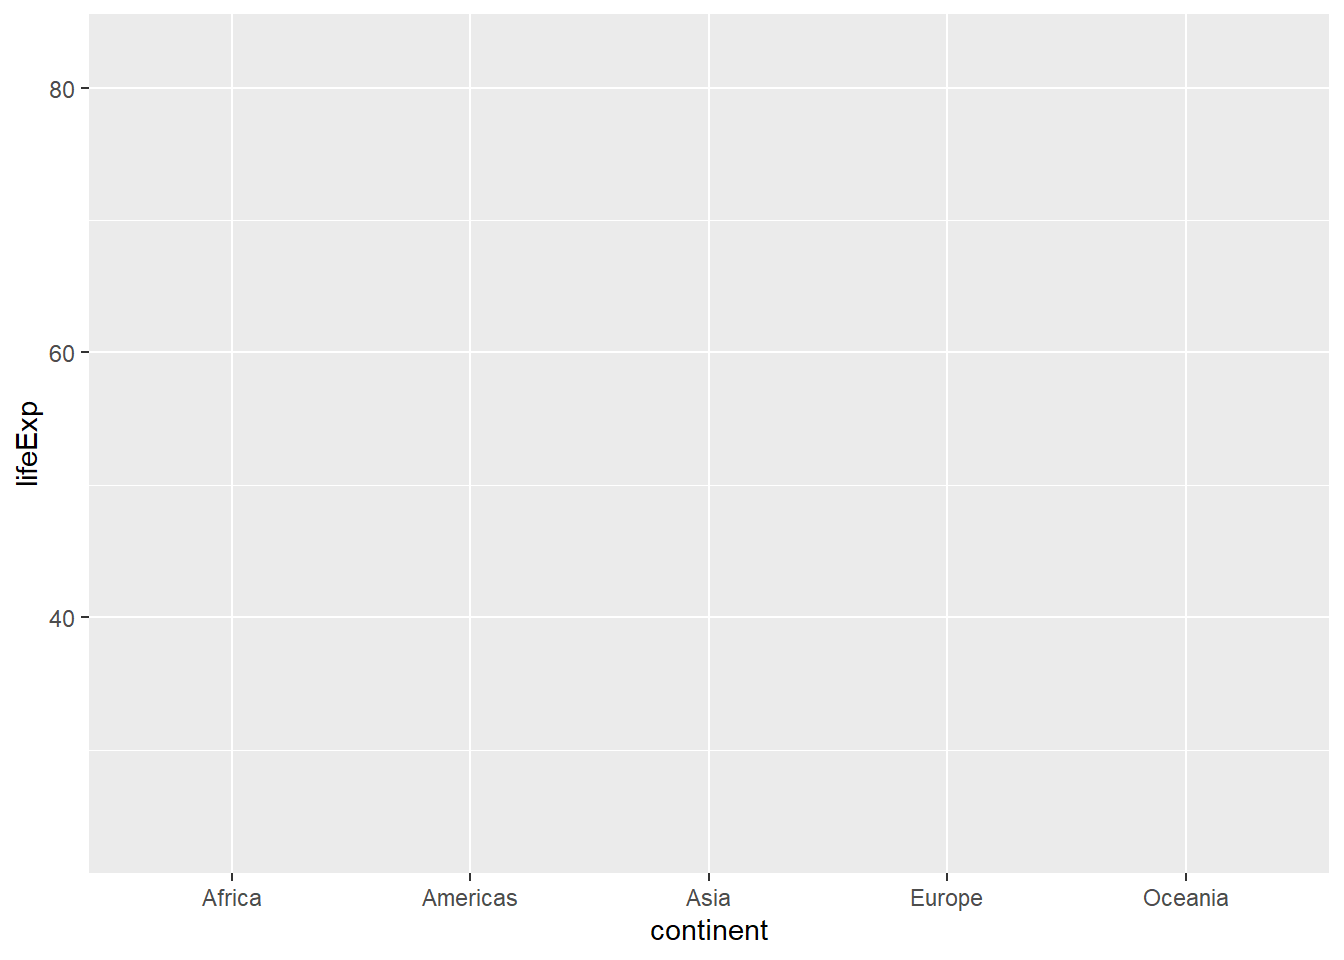
\includegraphics[width=0.8\linewidth]{2021-ASEE-Workshop_files/figure-latex/unnamed-chunk-55-1}

A box-and-whisker plot (or box plot) is designed for displaying the distribution of a single quantitative variable. The visual encoding is specified using the \texttt{geom\_boxplot()} layer, where a ``geom'' is a geometric object. The \texttt{geom\_boxplot()} function requires the quantitative variable assigned to \texttt{y} and the categorical variable (if any) to \texttt{x}.

\begin{Shaded}
\begin{Highlighting}[]
\CommentTok{\# Demonstrate adding a geometric object }
\NormalTok{life\_exp }\OtherTok{\textless{}{-}}\NormalTok{ life\_exp }\SpecialCharTok{+} 
  \FunctionTok{geom\_boxplot}\NormalTok{()}

\CommentTok{\# Examine the result}
\NormalTok{life\_exp}
\end{Highlighting}
\end{Shaded}

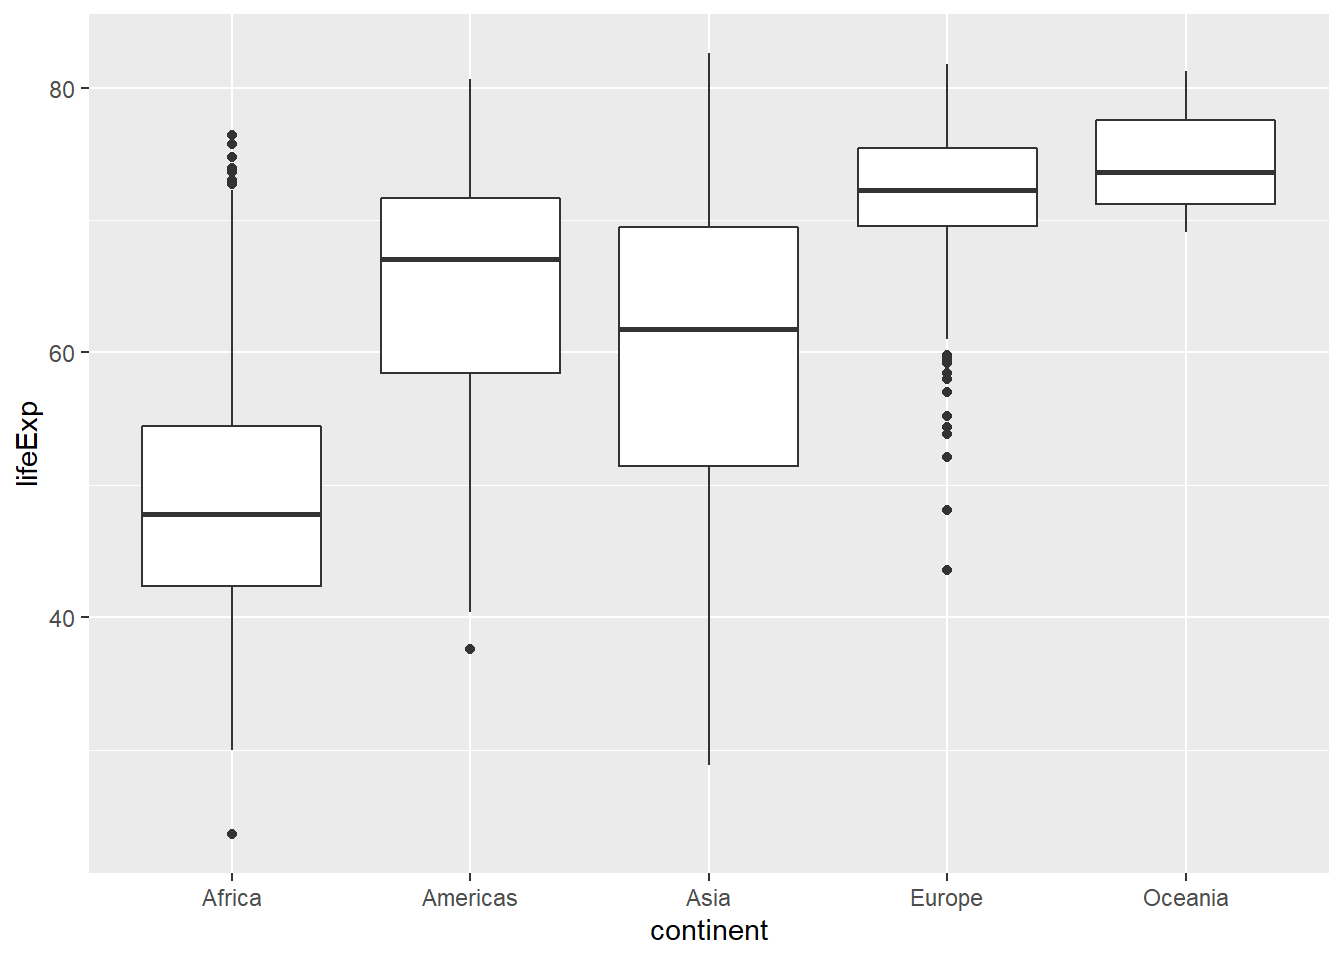
\includegraphics[width=0.8\linewidth]{2021-ASEE-Workshop_files/figure-latex/unnamed-chunk-56-1}

Notice that the default axis labels are the variables names from the data frame. We can edit those with another layer

\begin{Shaded}
\begin{Highlighting}[]
\CommentTok{\# Demonstrate editing axis labels}
\NormalTok{life\_exp }\OtherTok{\textless{}{-}}\NormalTok{ life\_exp }\SpecialCharTok{+} 
  \FunctionTok{labs}\NormalTok{(}\AttributeTok{x =} \StringTok{"Continent"}\NormalTok{, }\AttributeTok{y =} \StringTok{"Life expectancy (years)"}\NormalTok{)}

\CommentTok{\# Examine the result}
\NormalTok{life\_exp}
\end{Highlighting}
\end{Shaded}

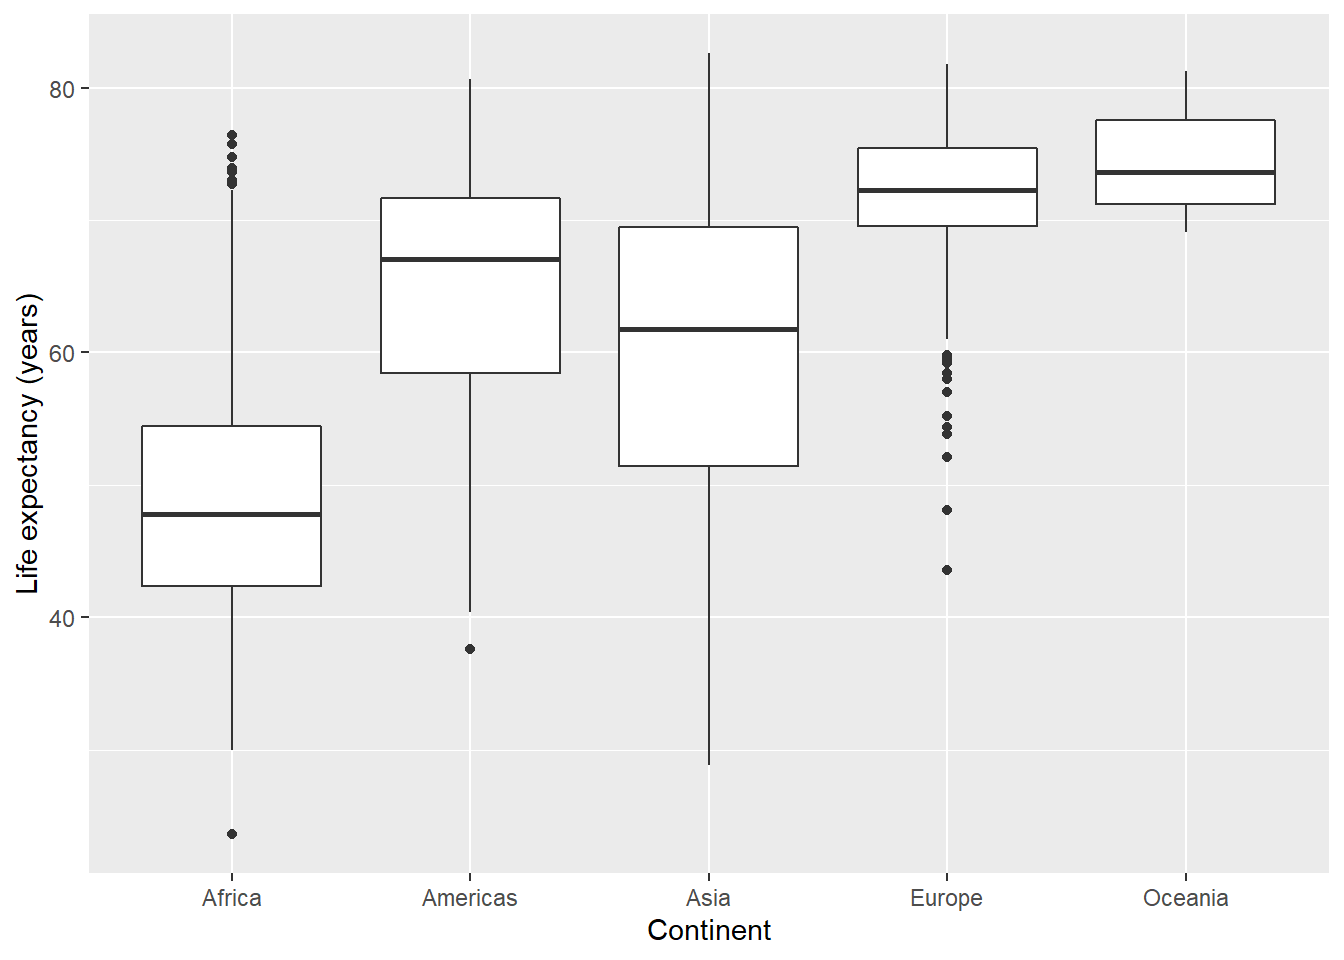
\includegraphics[width=0.8\linewidth]{2021-ASEE-Workshop_files/figure-latex/unnamed-chunk-57-1}

You can always write all the layers in one code chunk and obtain the same result.

\begin{Shaded}
\begin{Highlighting}[]
\CommentTok{\# Demonstrate all layers in one code chunk }
\NormalTok{p }\OtherTok{\textless{}{-}}  \FunctionTok{ggplot}\NormalTok{(}\AttributeTok{data =}\NormalTok{ gapminder, }\AttributeTok{mapping =} \FunctionTok{aes}\NormalTok{(}\AttributeTok{x =}\NormalTok{ continent, }\AttributeTok{y =}\NormalTok{ lifeExp)) }\SpecialCharTok{+}
  \FunctionTok{geom\_boxplot}\NormalTok{() }\SpecialCharTok{+}
  \FunctionTok{labs}\NormalTok{(}\AttributeTok{x =} \StringTok{"Continent"}\NormalTok{, }\AttributeTok{y =} \StringTok{"Life expectancy (years)"}\NormalTok{)}
\end{Highlighting}
\end{Shaded}

To reduce typing, the first two arguments \texttt{data} and \texttt{mapping} are often used without naming them explicitly, e.g.,

\begin{Shaded}
\begin{Highlighting}[]
\CommentTok{\# Demonstrate implicit data and mapping arguments}
\NormalTok{life\_exp }\OtherTok{\textless{}{-}}  \FunctionTok{ggplot}\NormalTok{(gapminder, }\FunctionTok{aes}\NormalTok{(}\AttributeTok{x =}\NormalTok{ continent, }\AttributeTok{y =}\NormalTok{ lifeExp)) }\SpecialCharTok{+}
  \FunctionTok{geom\_boxplot}\NormalTok{() }\SpecialCharTok{+}
  \FunctionTok{labs}\NormalTok{(}\AttributeTok{x =} \StringTok{"Continent"}\NormalTok{, }\AttributeTok{y =} \StringTok{"Life expectancy (years)"}\NormalTok{)}
\end{Highlighting}
\end{Shaded}

Next, we often want the categorical variable ordered by the quantitative variable instead of alphabetically. Because \texttt{continent} is a factor, we can use the \texttt{reorder()} function inside the \texttt{aes()} argument.

\begin{Shaded}
\begin{Highlighting}[]
\CommentTok{\# Demonstrate reordering a categorical variable }
\NormalTok{life\_exp }\SpecialCharTok{+} 
  \FunctionTok{aes}\NormalTok{(}\AttributeTok{x =} \FunctionTok{reorder}\NormalTok{(continent, lifeExp), }\AttributeTok{y =}\NormalTok{ lifeExp)}
\end{Highlighting}
\end{Shaded}

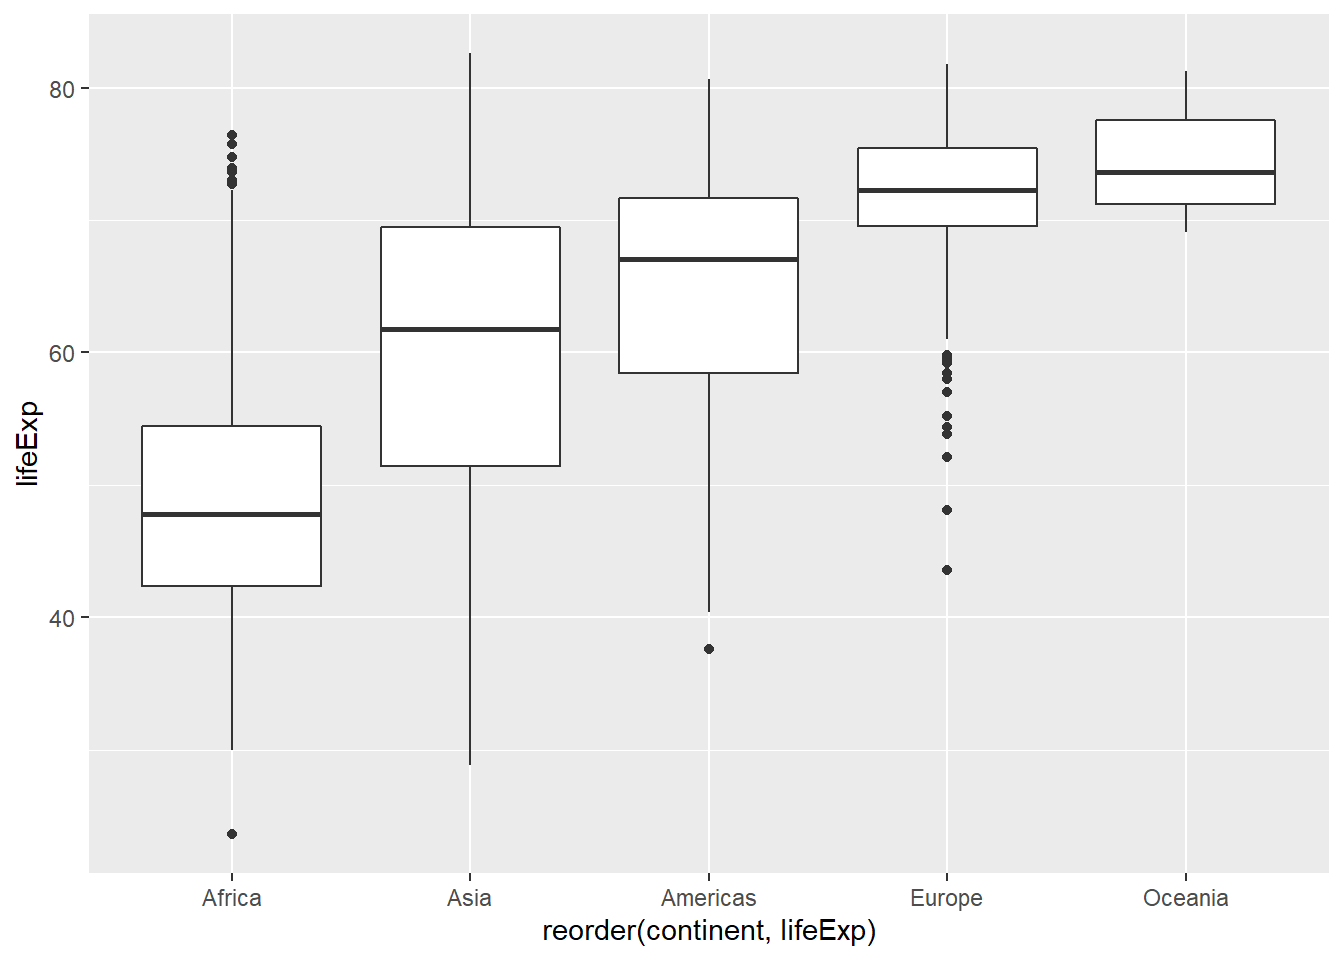
\includegraphics[width=0.8\linewidth]{2021-ASEE-Workshop_files/figure-latex/unnamed-chunk-60-1}

Summary. The basics steps for building up the layers of any graph consist of,

\begin{itemize}
\tightlist
\item
  assign the data frame
\item
  map variables (columns names) to aesthetic properties\\
\item
  choose geoms\\
\item
  adjust scales, labels, ordering, etc.
\end{itemize}

\hypertarget{exercise-1}{%
\subsection{Exercise}\label{exercise-1}}

\begin{itemize}
\tightlist
\item
  Examine the \texttt{term} data set from midfielddata.
\item
  Create a boxplot of the hours per term quantity conditioned by the student level.
\item
  What is the rational for leaving the categorical variable in its native order?
\item
  Check your work by comparing your result to the graph below.
\end{itemize}

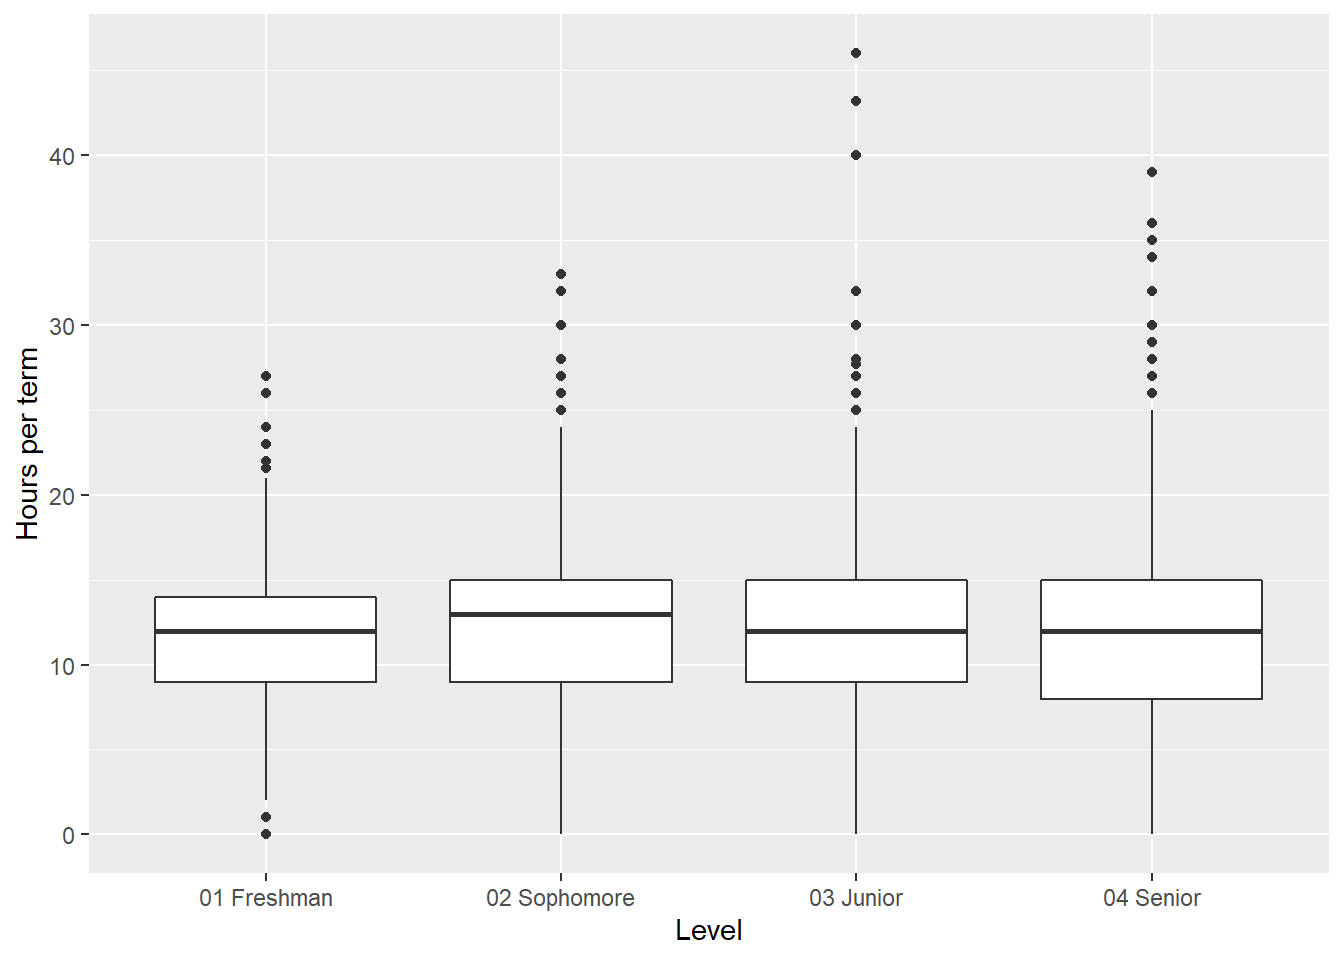
\includegraphics[width=0.8\linewidth]{2021-ASEE-Workshop_files/figure-latex/unnamed-chunk-61-1}

Help pages for more information:

\begin{itemize}
\tightlist
\item
  \href{https://midfieldr.github.io/midfielddata/reference/term.html}{\texttt{term}}
\item
  \href{https://ggplot2.tidyverse.org/reference/aes.html}{\texttt{aes()}}~\\
\item
  \href{https://ggplot2.tidyverse.org/reference/geom_boxplot.html}{\texttt{geom\_boxplot()}}
\item
  \href{https://ggplot2.tidyverse.org/reference/labs.html}{\texttt{geom\_labs()}}
\end{itemize}

\hypertarget{layer-points}{%
\section{Layer: points}\label{layer-points}}

A two-dimensional scatterplot reveals the strength of the relationship between two quantitative variables. The ggplot geom for scatterplots is \texttt{geom\_point()}. To illustrate a scatterplot, we graph life expectancy as a function of GDP.

\begin{Shaded}
\begin{Highlighting}[]
\NormalTok{life\_gdp }\OtherTok{\textless{}{-}} \FunctionTok{ggplot}\NormalTok{(gapminder, }\FunctionTok{aes}\NormalTok{(}\AttributeTok{x =}\NormalTok{ gdpPercap, }\AttributeTok{y =}\NormalTok{ lifeExp)) }\SpecialCharTok{+}
  \FunctionTok{geom\_point}\NormalTok{() }\SpecialCharTok{+}
  \FunctionTok{labs}\NormalTok{(}\AttributeTok{x =} \StringTok{"GDP per capita (USD)"}\NormalTok{, }\AttributeTok{y =} \StringTok{"Life expectancy (years)"}\NormalTok{)}

\NormalTok{life\_gdp}
\end{Highlighting}
\end{Shaded}

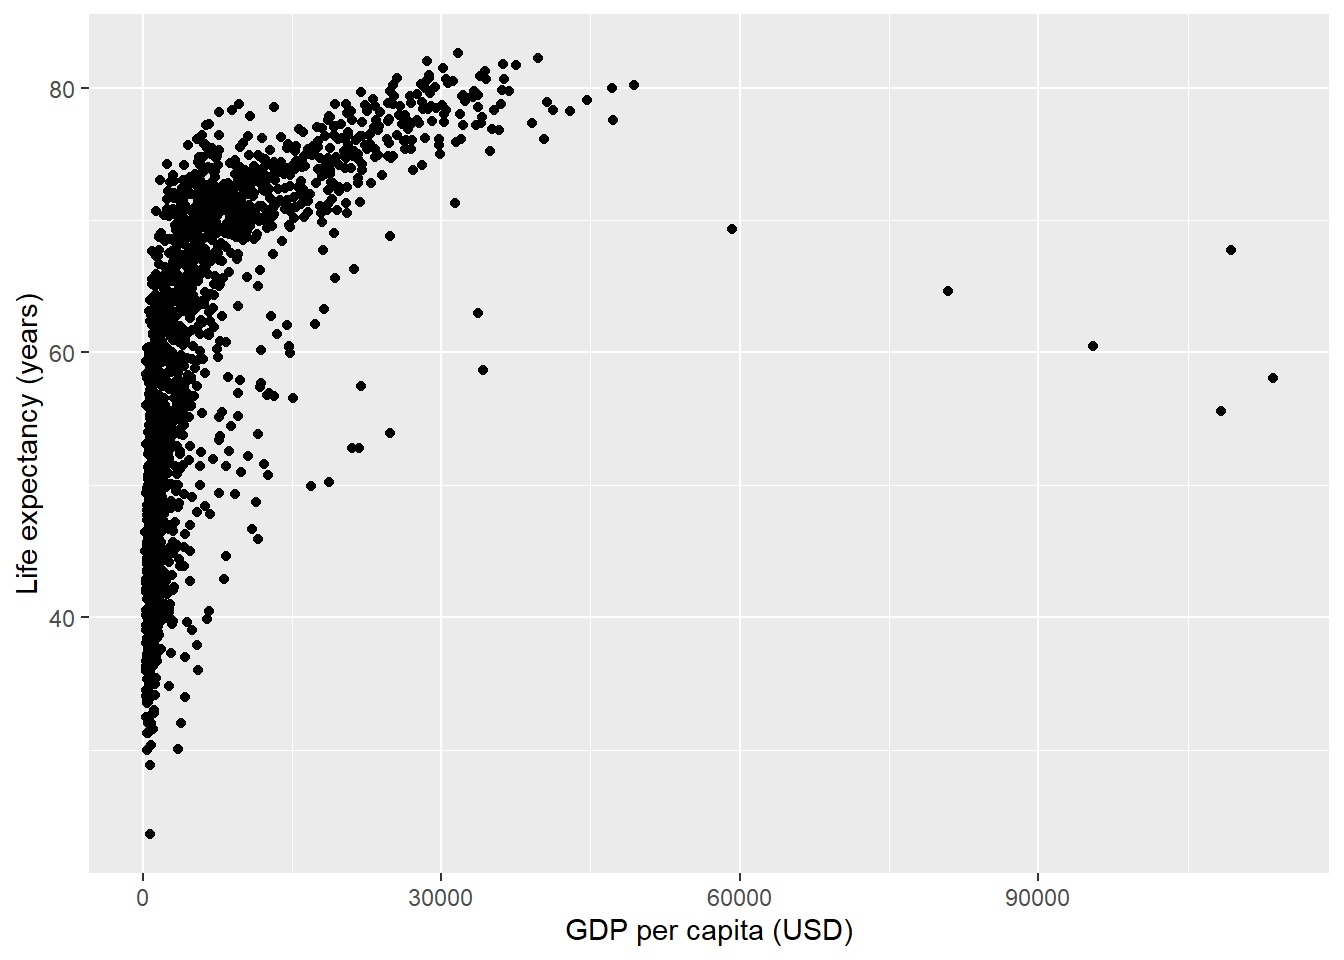
\includegraphics[width=0.8\linewidth]{2021-ASEE-Workshop_files/figure-latex/unnamed-chunk-62-1}

Help pages for more information:

\begin{itemize}
\tightlist
\item
  \href{https://ggplot2.tidyverse.org/reference/geom_point.html}{\texttt{geom\_point()}}
\end{itemize}

\hypertarget{layer-smooth-fit}{%
\section{Layer: smooth fit}\label{layer-smooth-fit}}

Suppose you wanted a smooth fit curve, not necessarily linear. Add a \texttt{geom\_smooth()} layer. The name \emph{loess} (pronounced like the proper name Lois) is a nonparametric curve-fitting method based on \emph{local regression}.

\begin{Shaded}
\begin{Highlighting}[]
\NormalTok{life\_gdp }\SpecialCharTok{+} 
  \FunctionTok{geom\_smooth}\NormalTok{(}\AttributeTok{method =} \StringTok{"loess"}\NormalTok{, }\AttributeTok{se =} \ConstantTok{FALSE}\NormalTok{)}
\end{Highlighting}
\end{Shaded}

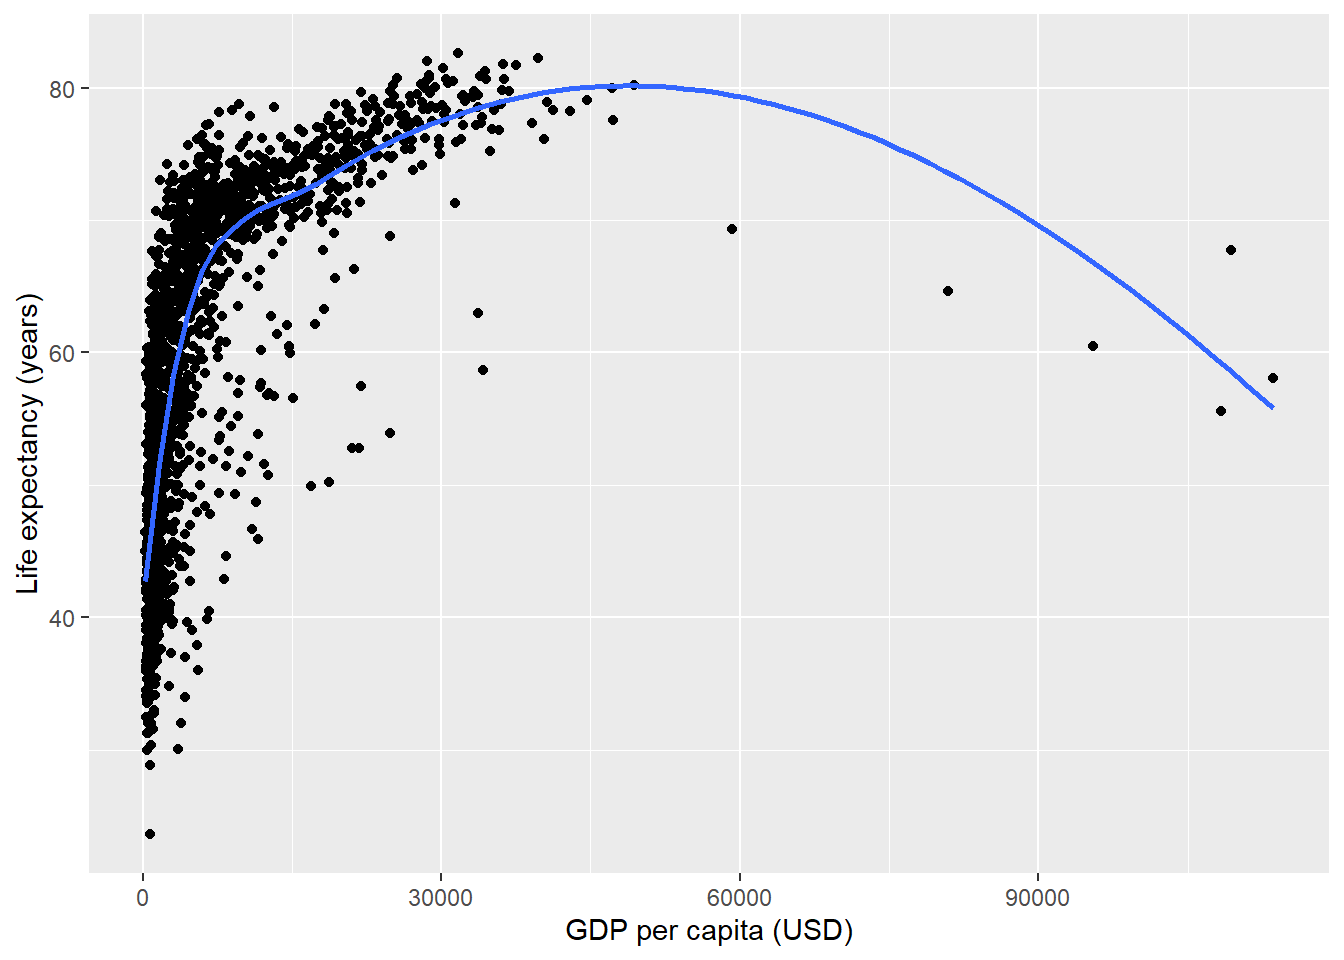
\includegraphics[width=0.8\linewidth]{2021-ASEE-Workshop_files/figure-latex/unnamed-chunk-63-1}

The \texttt{se} argument controls whether or not the confidence interval is displayed. Setting \texttt{se\ =\ TRUE} yields,

\begin{Shaded}
\begin{Highlighting}[]
\NormalTok{life\_gdp }\SpecialCharTok{+} 
  \FunctionTok{geom\_smooth}\NormalTok{(}\AttributeTok{method =} \StringTok{"loess"}\NormalTok{, }\AttributeTok{se =} \ConstantTok{TRUE}\NormalTok{)}
\end{Highlighting}
\end{Shaded}

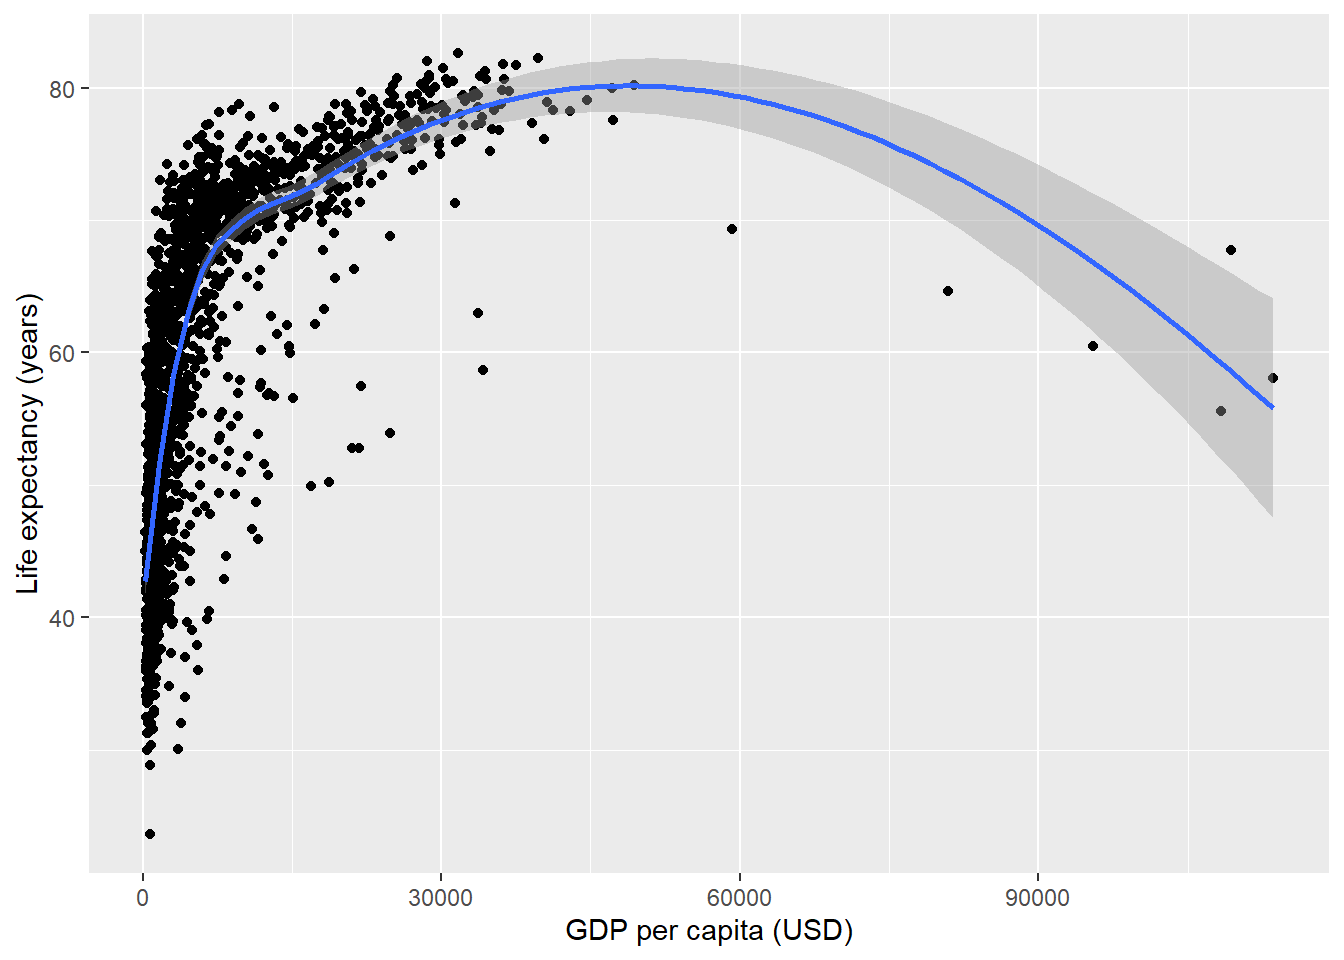
\includegraphics[width=0.8\linewidth]{2021-ASEE-Workshop_files/figure-latex/unnamed-chunk-64-1}

For a linear-fit layer, we add a layer with \texttt{method} set to \texttt{lm} (short for linear model). The linear fit is not particularly good in this case, but now you know how to do one.

\begin{Shaded}
\begin{Highlighting}[]
\NormalTok{life\_gdp }\SpecialCharTok{+} 
  \FunctionTok{geom\_smooth}\NormalTok{(}\AttributeTok{method =} \StringTok{"lm"}\NormalTok{, }\AttributeTok{se =} \ConstantTok{TRUE}\NormalTok{)}
\end{Highlighting}
\end{Shaded}

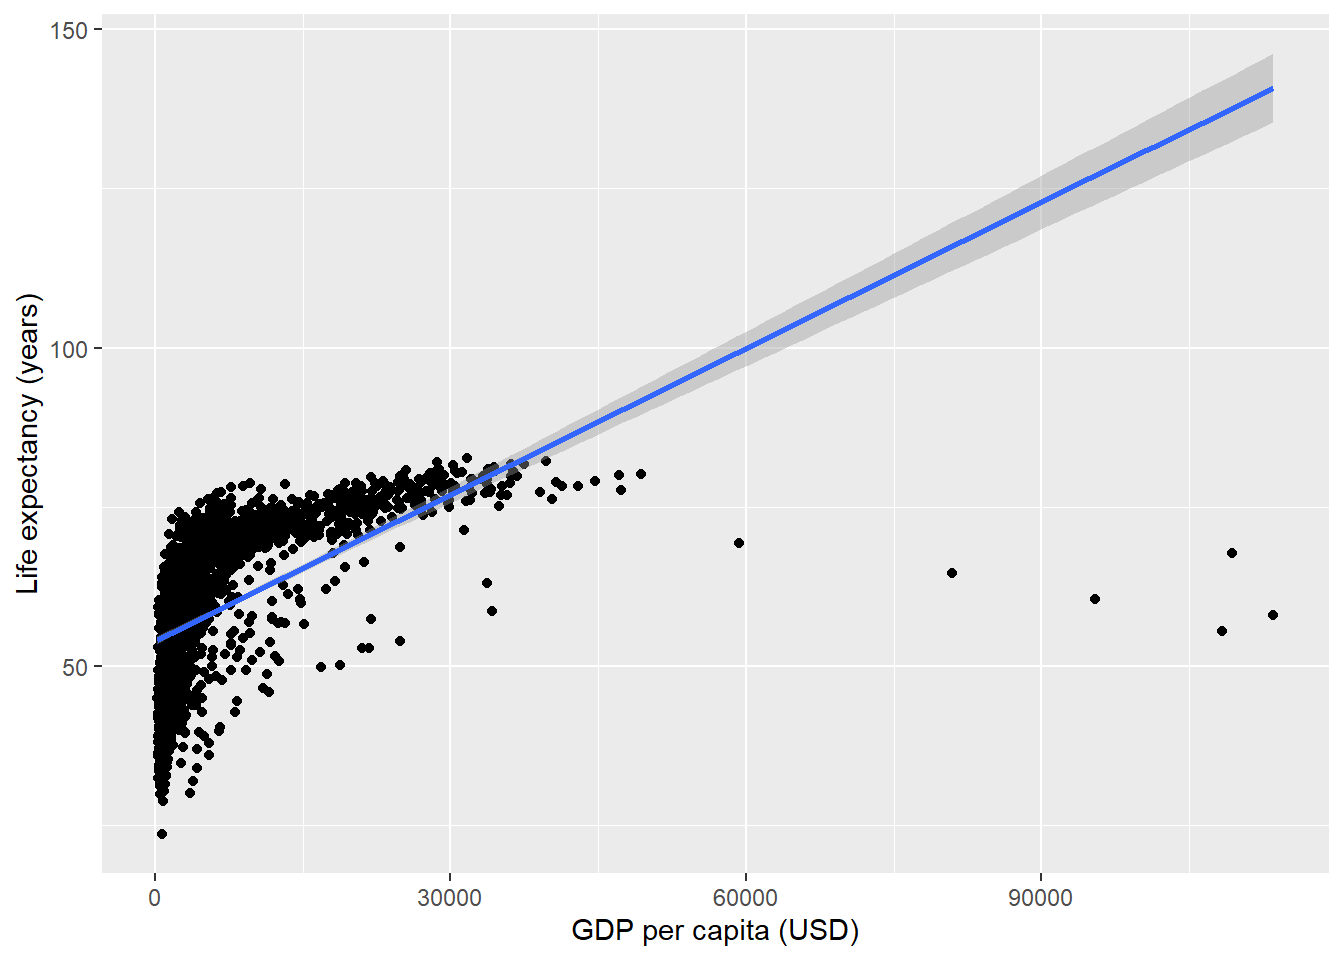
\includegraphics[width=0.8\linewidth]{2021-ASEE-Workshop_files/figure-latex/unnamed-chunk-65-1}

Help pages for more information:

\begin{itemize}
\tightlist
\item
  \href{https://ggplot2.tidyverse.org/reference/geom_smooth.html}{geom\_smooth()}
\end{itemize}

\hypertarget{exercise-2}{%
\subsection{Exercise}\label{exercise-2}}

In this exercise, we do some data manipulation without explaining the steps. We cover such details in the \protect\hyperlink{data-basics}{Data basics} tutorial. Here we are focusing on constructing graphs.

\begin{itemize}
\tightlist
\item
  Use the following code chunk to create a random sample of the \texttt{student} data set with columns for SAT math and verbal scores.
\end{itemize}

\begin{Shaded}
\begin{Highlighting}[]
\CommentTok{\# We only need two columns for the plot}
\NormalTok{cols\_we\_want }\OtherTok{\textless{}{-}} \FunctionTok{c}\NormalTok{(}\StringTok{"sat\_math"}\NormalTok{, }\StringTok{"sat\_verbal"}\NormalTok{)}
\NormalTok{sat }\OtherTok{\textless{}{-}}\NormalTok{ student[, ..cols\_we\_want]}

\CommentTok{\# Before sampling, we remove NA values }
\NormalTok{sat }\OtherTok{\textless{}{-}} \FunctionTok{na.omit}\NormalTok{(sat)}

\CommentTok{\# We sample to reduce computational time }
\NormalTok{sat }\OtherTok{\textless{}{-}}\NormalTok{ sat[}\FunctionTok{sample}\NormalTok{(}\FunctionTok{nrow}\NormalTok{(sat), }\DecValTok{3000}\NormalTok{)]}
\end{Highlighting}
\end{Shaded}

\begin{itemize}
\tightlist
\item
  Use the resulting \texttt{dtf} data frame and create a scatterplot of verbal scores \texttt{sat\_verbal} as a function of math scores \texttt{sat\_math}.\\
\item
  Add a loess fit.\\
\item
  Check your work by comparing your result to the graph below.
\end{itemize}

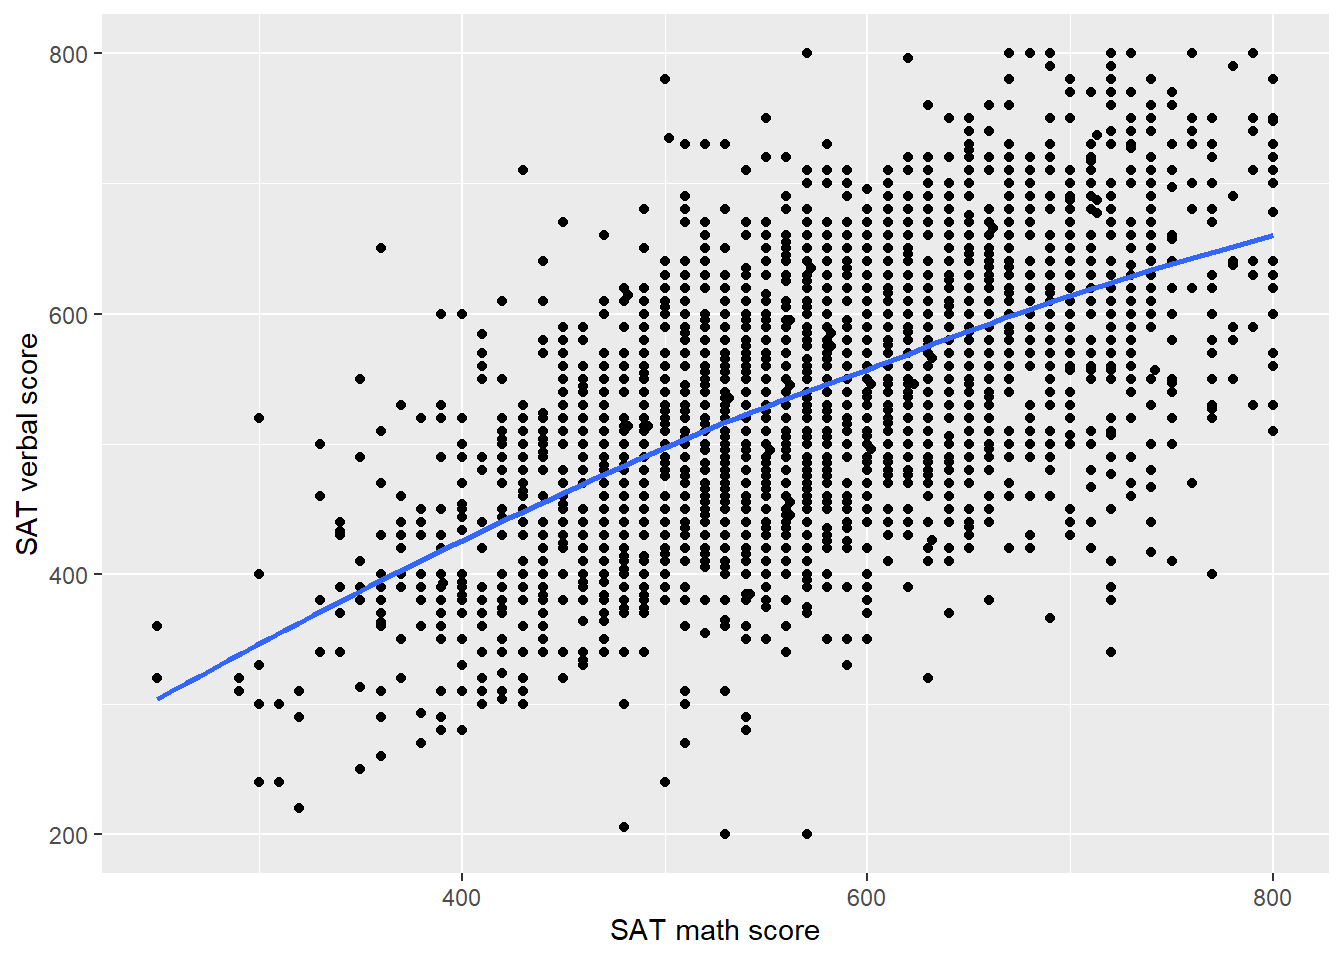
\includegraphics[width=0.8\linewidth]{2021-ASEE-Workshop_files/figure-latex/unnamed-chunk-67-1}

\hypertarget{layer-scale}{%
\section{Layer: scale}\label{layer-scale}}

We have orders of magnitude differences in the GDP per capita variable. To confirm, we can create a \texttt{summary()} of the \texttt{gdpPercap} variable. The output shows that the minimum is 241, the median 3532, and the maximum 113,523.

\begin{Shaded}
\begin{Highlighting}[]
\CommentTok{\# statistical summary of one variable }
\FunctionTok{summary}\NormalTok{(gapminder[, gdpPercap])}
\CommentTok{\#\textgreater{}     Min.  1st Qu.   Median     Mean  3rd Qu.     Max. }
\CommentTok{\#\textgreater{}    241.2   1202.1   3531.8   7215.3   9325.5 113523.1}
\end{Highlighting}
\end{Shaded}

In exploring a graph like this, it might be useful to add a layer that changes the horizontal scale to a log-base-10 scale.

\begin{Shaded}
\begin{Highlighting}[]
\NormalTok{life\_gdp }\OtherTok{\textless{}{-}}\NormalTok{ life\_gdp }\SpecialCharTok{+}
  \FunctionTok{scale\_x\_continuous}\NormalTok{(}\AttributeTok{trans =} \StringTok{"log10"}\NormalTok{) }
\end{Highlighting}
\end{Shaded}

Update the axis labels,

\begin{Shaded}
\begin{Highlighting}[]
\NormalTok{life\_gdp }\OtherTok{\textless{}{-}}\NormalTok{ life\_gdp }\SpecialCharTok{+}
  \FunctionTok{labs}\NormalTok{(}\AttributeTok{x =} \StringTok{"GDP per capita, USD (log10 scale)"}\NormalTok{, }
       \AttributeTok{y =} \StringTok{"Life expectancy (years)"}\NormalTok{)}

\NormalTok{life\_gdp }\CommentTok{\# display the graph}
\end{Highlighting}
\end{Shaded}

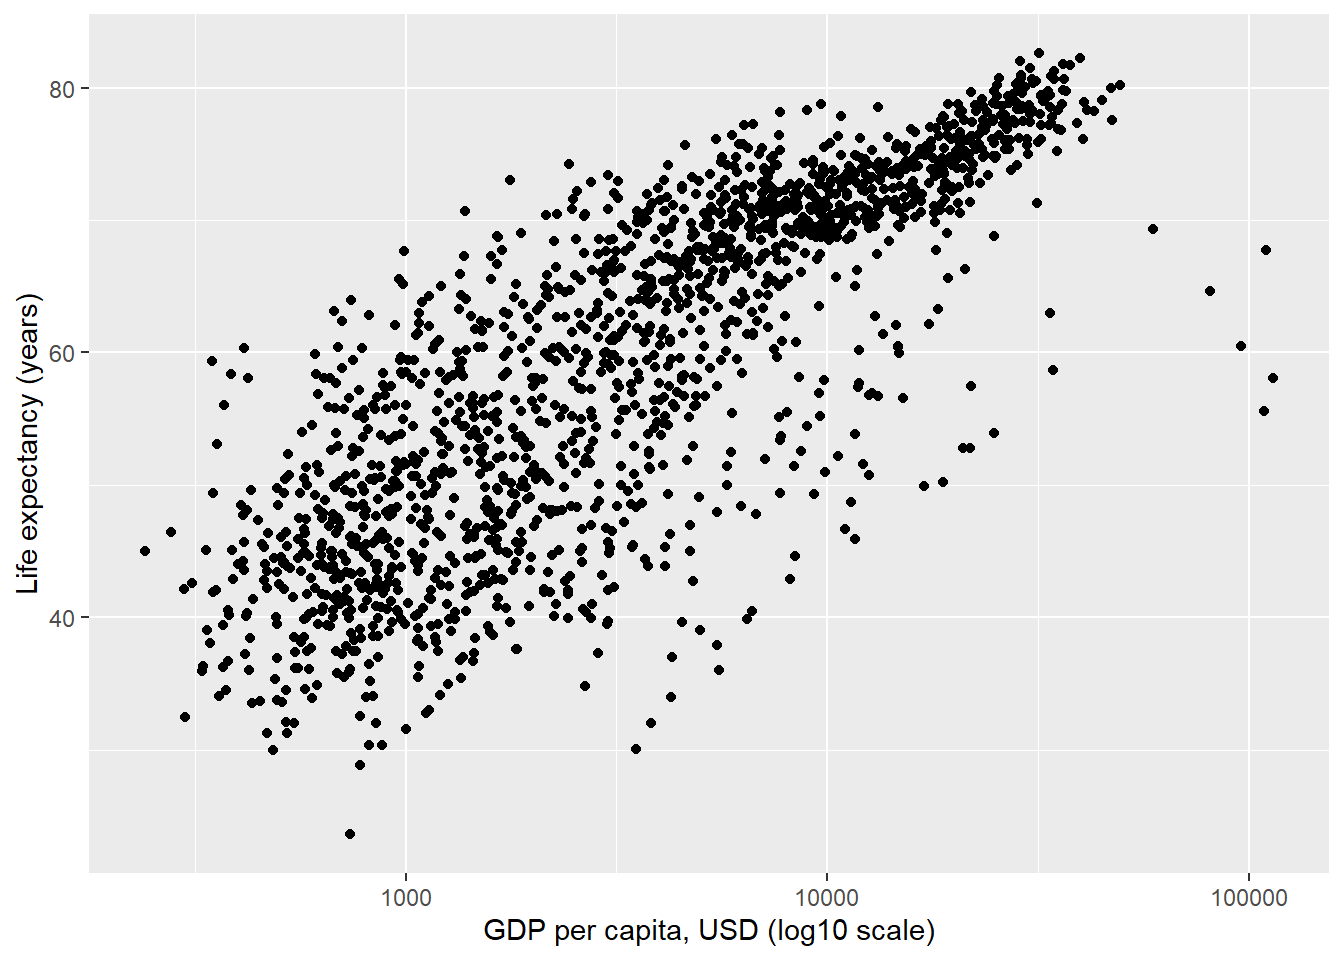
\includegraphics[width=0.8\linewidth]{2021-ASEE-Workshop_files/figure-latex/unnamed-chunk-71-1}

In summary, all the layers could have been be coded at once, for example,

\begin{Shaded}
\begin{Highlighting}[]
\FunctionTok{ggplot}\NormalTok{(gapminder, }\FunctionTok{aes}\NormalTok{(}\AttributeTok{x =}\NormalTok{ gdpPercap, }\AttributeTok{y =}\NormalTok{ lifeExp)) }\SpecialCharTok{+}
  \FunctionTok{geom\_point}\NormalTok{() }\SpecialCharTok{+}
  \FunctionTok{scale\_x\_continuous}\NormalTok{(}\AttributeTok{trans =} \StringTok{"log10"}\NormalTok{) }\SpecialCharTok{+}
  \FunctionTok{labs}\NormalTok{(}\AttributeTok{x =} \StringTok{"GDP per capita, USD (log10 scale)"}\NormalTok{, }
       \AttributeTok{y =} \StringTok{"Life expectancy (years)"}\NormalTok{)}
\end{Highlighting}
\end{Shaded}

With all the layers in one place, we can see that we've coded all the basic steps, that is,

\begin{itemize}
\tightlist
\item
  assign the data frame\\
\item
  map variables (columns names) to aesthetic properties\\
\item
  choose geoms\\
\item
  adjust scales, labels, ordering, etc.
\end{itemize}

\hypertarget{exercise-3}{%
\subsection{Exercise}\label{exercise-3}}

Again we do some data manipulation without explaining the steps. We cover such details in the \protect\hyperlink{data-basics}{Data basics} tutorial. Here we are focusing on constructing graphs.

We often use graphs to show numbers of students with a log-scale to compare totals that differ by orders of magnitude.

\begin{itemize}
\tightlist
\item
  Use the following code chunk to count the number students ever enrolled in the sample data by race/ethnicity/sex.
\end{itemize}

\begin{Shaded}
\begin{Highlighting}[]
\CommentTok{\# Access a data set included with midfieldr}
\NormalTok{dtf }\OtherTok{\textless{}{-}} \FunctionTok{copy}\NormalTok{(study\_stickiness)}

\CommentTok{\# Create a combined categorical column }
\NormalTok{dtf[, race\_sex }\SpecialCharTok{:}\ErrorTok{=} \FunctionTok{paste}\NormalTok{(race, sex)]}

\CommentTok{\# Sum the number of students by this category }
\NormalTok{dtf[, ever }\SpecialCharTok{:}\ErrorTok{=} \FunctionTok{sum}\NormalTok{(ever), by }\OtherTok{=} \StringTok{"race\_sex"}\NormalTok{]}

\CommentTok{\# Factor class enables reordering }
\NormalTok{dtf[, race\_sex }\SpecialCharTok{:}\ErrorTok{=} \FunctionTok{factor}\NormalTok{(race\_sex)]}
\end{Highlighting}
\end{Shaded}

\begin{itemize}
\tightlist
\item
  Use the resulting \texttt{dtf} data frame to graph \texttt{ever} on the x-axis with \texttt{race\_sex} on the y-axis.\\
\item
  Reorder \texttt{race\_sex} by \texttt{ever}.\\
\item
  Use a log-base-2 scale.\\
\item
  You can omit the y-axis label by setting \texttt{y\ =\ ""} in the \texttt{labs()} argument.\\
\item
  Check your work by comparing your result to the graph below.
\end{itemize}

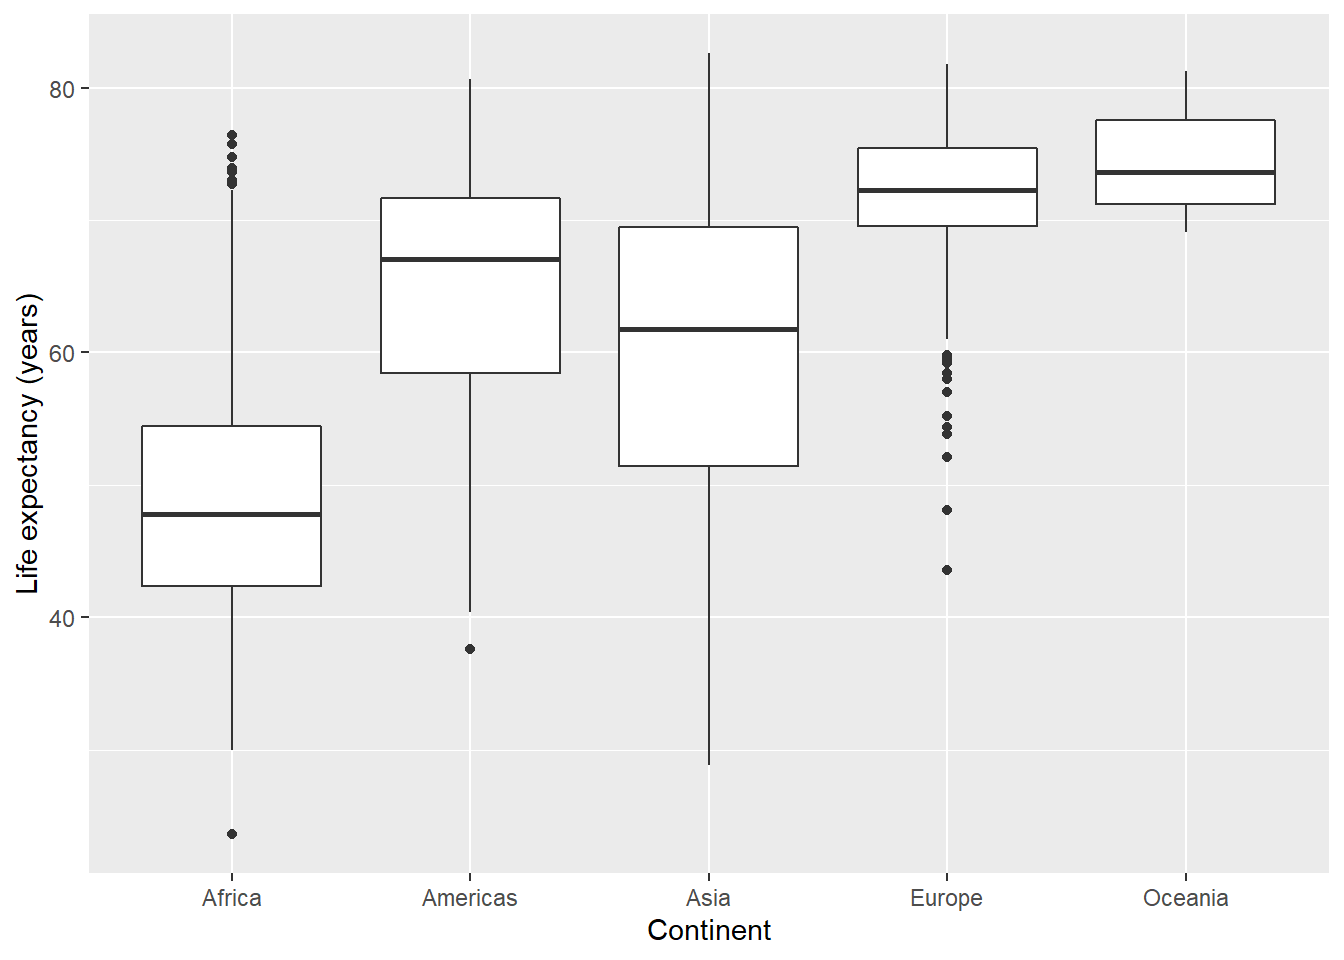
\includegraphics[width=0.8\linewidth]{2021-ASEE-Workshop_files/figure-latex/unnamed-chunk-74-1}

Help pages for more information:

\begin{itemize}
\tightlist
\item
  \href{https://ggplot2.tidyverse.org/reference/scale_continuous.html}{scale\_x\_continuous()}
\end{itemize}

\hypertarget{mapping-columns-to-aesthetics}{%
\section{Mapping columns to aesthetics}\label{mapping-columns-to-aesthetics}}

Mappings in the \texttt{aes()} function of \texttt{ggplot()} can involve the names of variables (column s) only. So far, the only mappings we've used are from column names to an x or y aesthetic.

Another useful mapping is from a column name to the \texttt{color} argument, which then separates the data by the values of the categorical variable selected and automatically creates the appropriate legend.

Here we map the \texttt{continent} column to the \texttt{color} aesthetic, adding a third data variable to the display.

\begin{Shaded}
\begin{Highlighting}[]
\FunctionTok{ggplot}\NormalTok{(gapminder, }\FunctionTok{aes}\NormalTok{(}\AttributeTok{x =}\NormalTok{ gdpPercap, }\AttributeTok{y =}\NormalTok{ lifeExp, }\AttributeTok{color =}\NormalTok{ continent)) }\SpecialCharTok{+}
  \FunctionTok{geom\_point}\NormalTok{() }\SpecialCharTok{+}
  \FunctionTok{scale\_x\_continuous}\NormalTok{(}\AttributeTok{trans =} \StringTok{"log10"}\NormalTok{) }\SpecialCharTok{+}
  \FunctionTok{labs}\NormalTok{(}\AttributeTok{x =} \StringTok{"GDP per capita, USD (log10 scale)"}\NormalTok{, }
       \AttributeTok{y =} \StringTok{"Life expectancy (years)"}\NormalTok{)}
\end{Highlighting}
\end{Shaded}

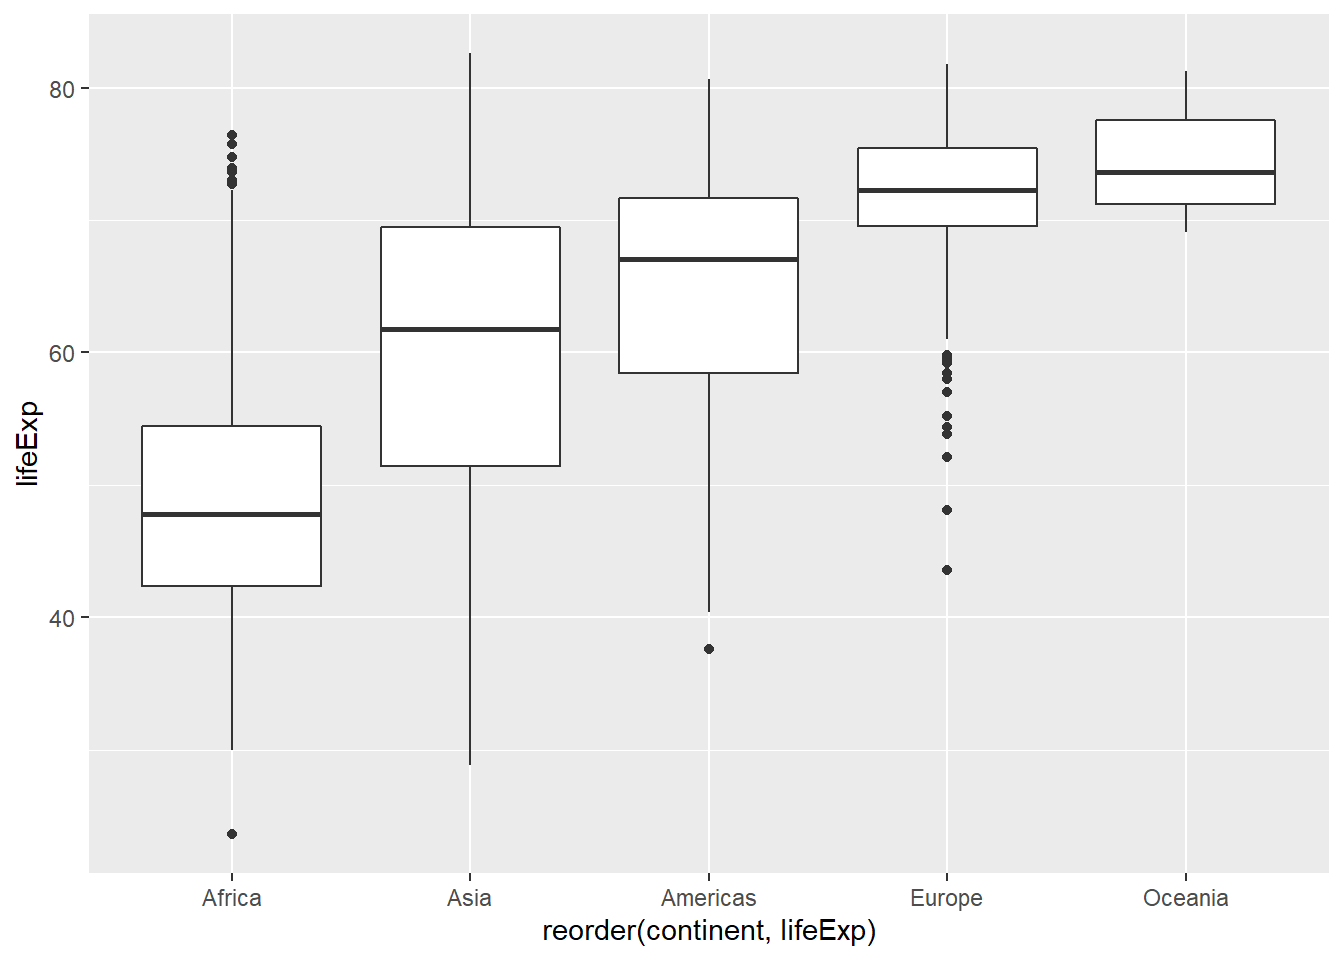
\includegraphics[width=0.8\linewidth]{2021-ASEE-Workshop_files/figure-latex/unnamed-chunk-75-1}

\hypertarget{exercise-4}{%
\subsection{Exercise}\label{exercise-4}}

Use the following code chunk to construct a data frame with hours per term and level from \texttt{term} merged with \texttt{sex} data from \texttt{student}. Again, we leave explanations of the data manipulation to the \protect\hyperlink{data-basics}{Data basics} tutorial.

\begin{Shaded}
\begin{Highlighting}[]
\NormalTok{dtf }\OtherTok{\textless{}{-}} \FunctionTok{add\_race\_sex}\NormalTok{(term, }
                    \AttributeTok{midfield\_student =}\NormalTok{ student)}
\NormalTok{cols\_we\_want }\OtherTok{\textless{}{-}} \FunctionTok{c}\NormalTok{(}\StringTok{"mcid"}\NormalTok{, }\StringTok{"term"}\NormalTok{, }\StringTok{"hours\_term"}\NormalTok{, }\StringTok{"level"}\NormalTok{, }\StringTok{"sex"}\NormalTok{)}
\NormalTok{dtf }\OtherTok{\textless{}{-}}\NormalTok{ dtf[, ..cols\_we\_want]}
\NormalTok{dtf }\OtherTok{\textless{}{-}} \FunctionTok{unique}\NormalTok{(dtf)}
\end{Highlighting}
\end{Shaded}

\begin{itemize}
\tightlist
\item
  Use the resulting \texttt{dtf} data frame to a boxplot of hours per term as a function of level like we did earlier.
\item
  Add a third column name to \texttt{aes()} to add \texttt{sex} by color to the graph.
\item
  Add the \texttt{coord\_flip()} layer to your graph to swap the position of the x, y coordinates to obtain a horizontal boxplot.
\item
  Check your work by comparing your result to the graph below.
\end{itemize}

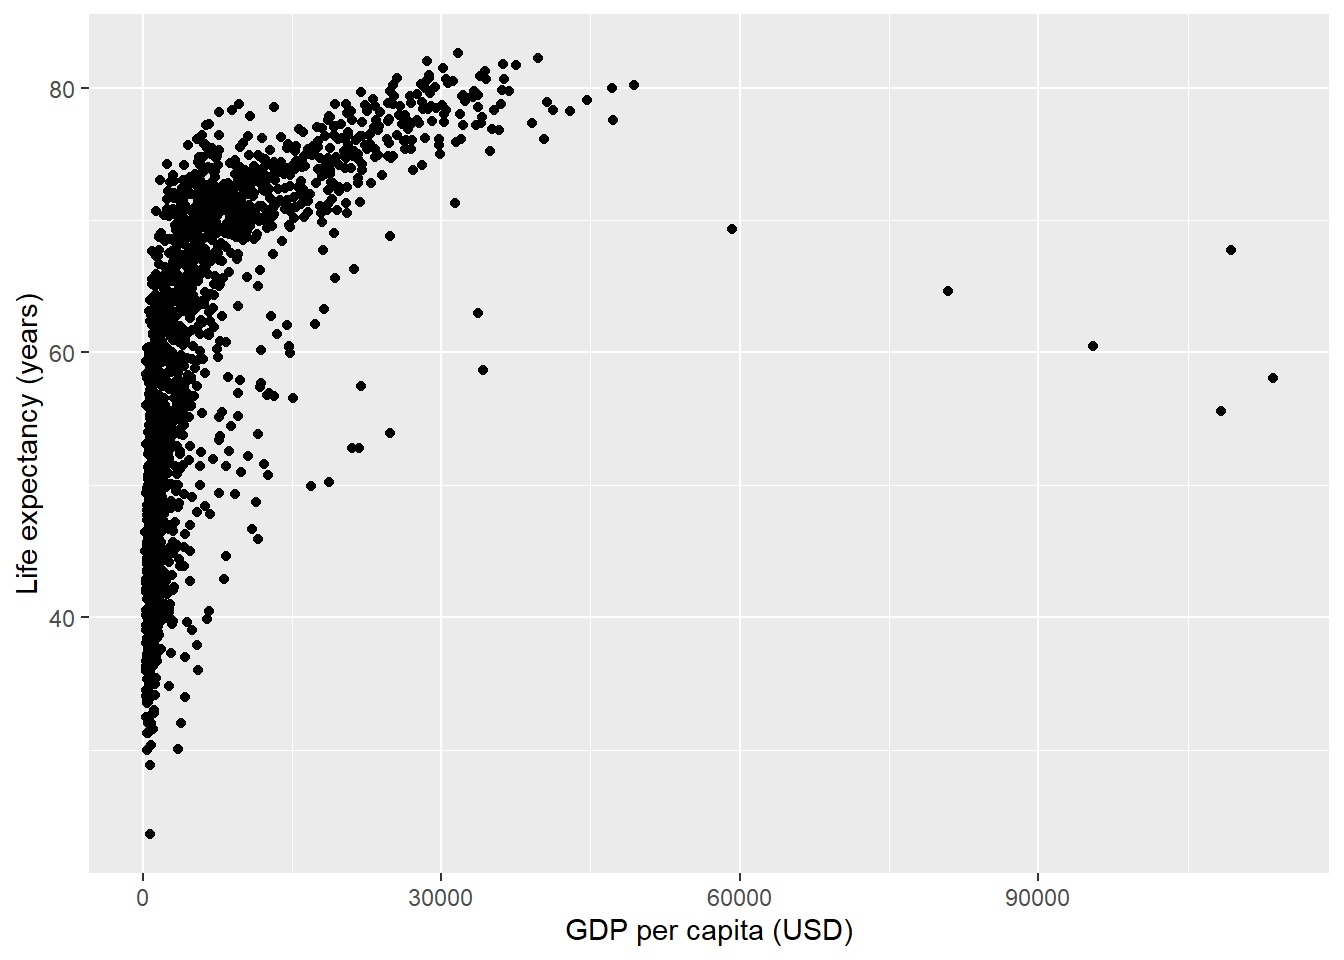
\includegraphics[width=0.8\linewidth]{2021-ASEE-Workshop_files/figure-latex/unnamed-chunk-77-1}

Help pages for more information:

\begin{itemize}
\tightlist
\item
  \href{https://midfieldr.github.io/midfieldr/reference/add_race_sex.html}{\texttt{add\_race\_sex()}}
\item
  \href{https://ggplot2.tidyverse.org/reference/coord_flip.html}{\texttt{coord\_flip()}}
\end{itemize}

\hypertarget{layer-facets}{%
\section{Layer: facets}\label{layer-facets}}

In the earlier graph where we mapped continent to color, there was a lot of overprinting, making it difficult to compare the continents. Instead of using color to distinguish the continents, we can plot in different panels by continent.

The \texttt{facet\_wrap()} layer separates the data into different panels (or facets). Like the \texttt{aes()} mapping, \texttt{facet\_wrap()} is applied to a variable (column name) in the data frame.

\begin{Shaded}
\begin{Highlighting}[]
\NormalTok{life\_gdp }\OtherTok{\textless{}{-}}\NormalTok{ life\_gdp }\SpecialCharTok{+} 
  \FunctionTok{facet\_wrap}\NormalTok{(}\AttributeTok{facets =} \FunctionTok{vars}\NormalTok{(continent))}

\NormalTok{life\_gdp }\CommentTok{\# print the graph}
\end{Highlighting}
\end{Shaded}

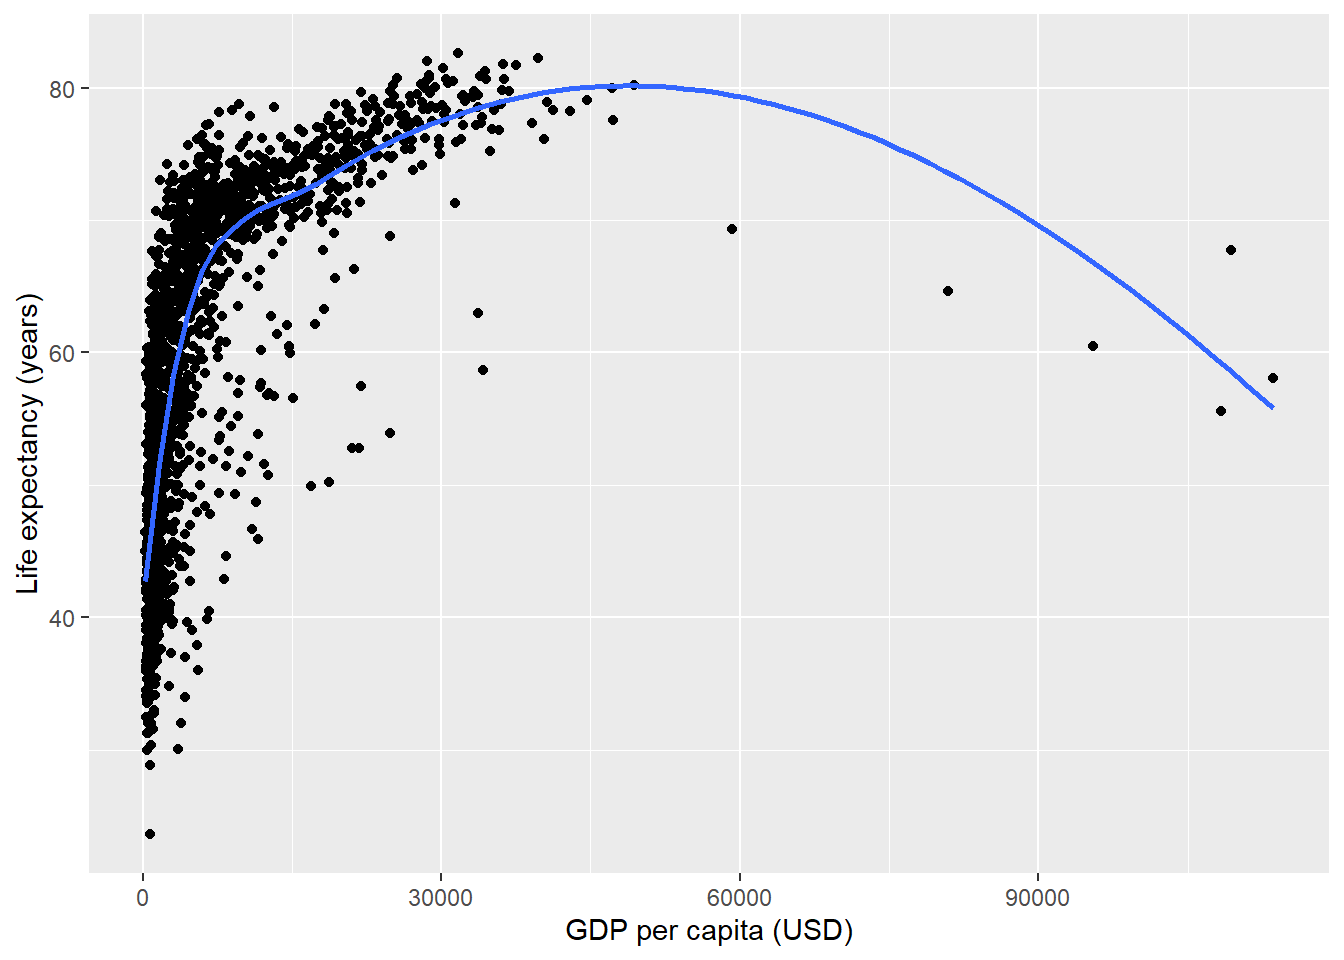
\includegraphics[width=0.8\linewidth]{2021-ASEE-Workshop_files/figure-latex/unnamed-chunk-78-1}

Comparisons are facilitated by having the facets appear in one column, by using the \texttt{ncol} argument of \texttt{facet\_wrap()}.

\begin{Shaded}
\begin{Highlighting}[]
\NormalTok{life\_gdp }\OtherTok{\textless{}{-}}\NormalTok{ life\_gdp }\SpecialCharTok{+} \FunctionTok{facet\_wrap}\NormalTok{(}\AttributeTok{facets =} \FunctionTok{vars}\NormalTok{(continent), }\AttributeTok{ncol =} \DecValTok{1}\NormalTok{)}

\NormalTok{life\_gdp }\CommentTok{\# print the graph}
\end{Highlighting}
\end{Shaded}

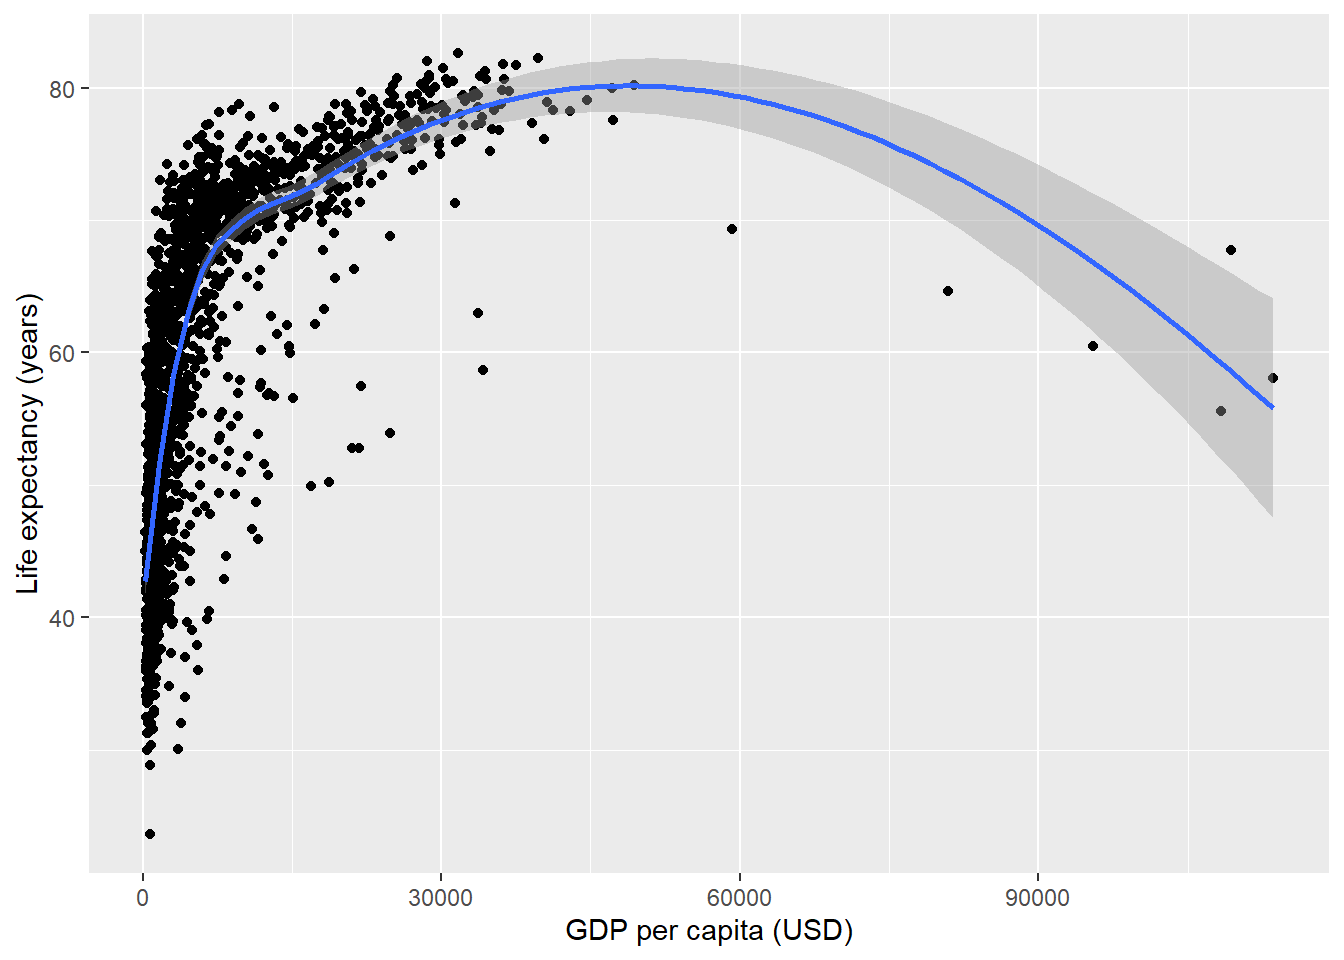
\includegraphics[width=0.8\linewidth]{2021-ASEE-Workshop_files/figure-latex/unnamed-chunk-79-1}

In a faceted display, all panels have identical scales (the default) to facilitate comparison. Again, all the layers could have been be coded at once, for example,

\begin{Shaded}
\begin{Highlighting}[]
\FunctionTok{ggplot}\NormalTok{(gapminder, }\FunctionTok{aes}\NormalTok{(}\AttributeTok{x =}\NormalTok{ gdpPercap, }\AttributeTok{y =}\NormalTok{ lifeExp)) }\SpecialCharTok{+}
  \FunctionTok{facet\_wrap}\NormalTok{(}\AttributeTok{facets =} \FunctionTok{vars}\NormalTok{(continent), }\AttributeTok{ncol =} \DecValTok{1}\NormalTok{) }\SpecialCharTok{+}
  \FunctionTok{geom\_point}\NormalTok{() }\SpecialCharTok{+}
  \FunctionTok{scale\_x\_continuous}\NormalTok{(}\AttributeTok{trans =} \StringTok{"log10"}\NormalTok{) }\SpecialCharTok{+}
  \FunctionTok{labs}\NormalTok{(}\AttributeTok{x =} \StringTok{"GDP per capita, USD (log10 scale)"}\NormalTok{, }
       \AttributeTok{y =} \StringTok{"Life expectancy (years)"}\NormalTok{) }
\end{Highlighting}
\end{Shaded}

\hypertarget{exercise-5}{%
\subsection{Exercise}\label{exercise-5}}

Use the following code chunk to construct a data frame of program stickiness by program, race/ethnicity, and sex.

\begin{Shaded}
\begin{Highlighting}[]
\CommentTok{\# Access a data set included with midfieldr}
\NormalTok{stickiness }\OtherTok{\textless{}{-}} \FunctionTok{copy}\NormalTok{(study\_stickiness)}

\CommentTok{\# Create a combined categorical column }
\NormalTok{stickiness[, race\_sex }\SpecialCharTok{:}\ErrorTok{=} \FunctionTok{paste}\NormalTok{(race, sex)]}

\CommentTok{\# Factor class enables reordering }
\NormalTok{stickiness[, race\_sex }\SpecialCharTok{:}\ErrorTok{=} \FunctionTok{factor}\NormalTok{(race\_sex)]}
\NormalTok{stickiness[, program }\SpecialCharTok{:}\ErrorTok{=} \FunctionTok{factor}\NormalTok{(program)]}

\CommentTok{\# Omit ambiguous race/ethnicities and small populations}
\NormalTok{stickiness }\OtherTok{\textless{}{-}}\NormalTok{ stickiness[}\SpecialCharTok{!}\NormalTok{race\_sex }\SpecialCharTok{\%ilike\%} \FunctionTok{c}\NormalTok{(}\StringTok{"Native|International|Other"}\NormalTok{)]}
\end{Highlighting}
\end{Shaded}

\begin{itemize}
\tightlist
\item
  Use the resulting \texttt{dtf} data frame plot stickiness (x-axis) as a function of race/ethnicity/sex (y-axis) and faceted by program.\\
\item
  When that graph seems OK, add a third column name to \texttt{aes()} to add \texttt{sex} by color to the graph.
\item
  Check your work by comparing your result to the graph below.
\end{itemize}

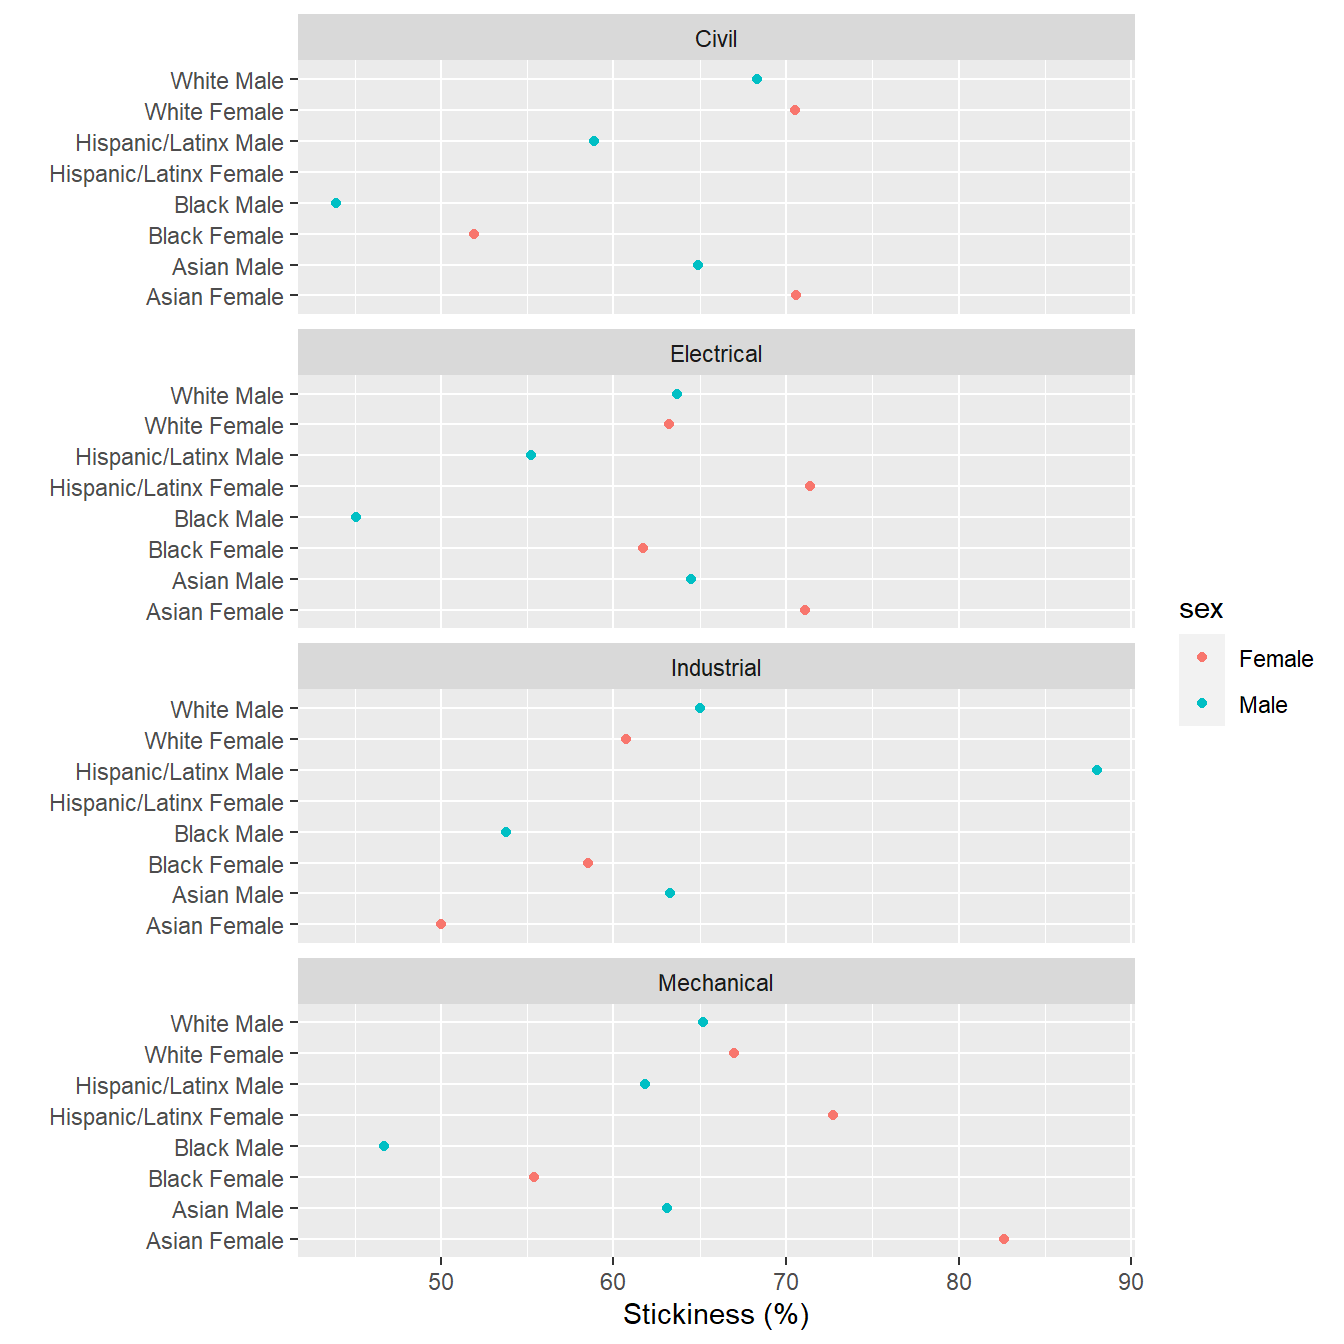
\includegraphics[width=0.8\linewidth]{2021-ASEE-Workshop_files/figure-latex/unnamed-chunk-82-1}

Help pages for more information:

\begin{itemize}
\tightlist
\item
  \href{https://ggplot2.tidyverse.org/reference/facet_wrap.html}{facet\_wrap()}
\end{itemize}

\hypertarget{ordering-panels-and-rows}{%
\section{Ordering panels and rows}\label{ordering-panels-and-rows}}

Panels (facets) by default are nearly always ordered alphabetically. In most cases, ordering the panels by the data improves the display. Earlier, we used \texttt{reorder()} to order a set of boxplots. This function operates correctly on ``factor'' variables only.

A factor is special data structure in R for categorical variables. In a factor, the levels of the category---typically character strings---are known and fixed. However, factors are stored internally as integers---a critical design tool for meaningfully ordering the rows and panels of a display involving categorical variables.

In the gapminder data, the \texttt{continent} column is already a factors.

\begin{Shaded}
\begin{Highlighting}[]
\NormalTok{gapminder}
\CommentTok{\#\textgreater{}           country continent  year lifeExp      pop gdpPercap}
\CommentTok{\#\textgreater{}            \textless{}fctr\textgreater{}    \textless{}fctr\textgreater{} \textless{}int\textgreater{}   \textless{}num\textgreater{}    \textless{}int\textgreater{}     \textless{}num\textgreater{}}
\CommentTok{\#\textgreater{}    1: Afghanistan      Asia  1952  28.801  8425333  779.4453}
\CommentTok{\#\textgreater{}    2: Afghanistan      Asia  1957  30.332  9240934  820.8530}
\CommentTok{\#\textgreater{}    3: Afghanistan      Asia  1962  31.997 10267083  853.1007}
\CommentTok{\#\textgreater{}    4: Afghanistan      Asia  1967  34.020 11537966  836.1971}
\CommentTok{\#\textgreater{}    5: Afghanistan      Asia  1972  36.088 13079460  739.9811}
\CommentTok{\#\textgreater{}   {-}{-}{-}                                                       }
\CommentTok{\#\textgreater{} 1700:    Zimbabwe    Africa  1987  62.351  9216418  706.1573}
\CommentTok{\#\textgreater{} 1701:    Zimbabwe    Africa  1992  60.377 10704340  693.4208}
\CommentTok{\#\textgreater{} 1702:    Zimbabwe    Africa  1997  46.809 11404948  792.4500}
\CommentTok{\#\textgreater{} 1703:    Zimbabwe    Africa  2002  39.989 11926563  672.0386}
\CommentTok{\#\textgreater{} 1704:    Zimbabwe    Africa  2007  43.487 12311143  469.7093}
\end{Highlighting}
\end{Shaded}

We can reorder the levels of the factor before graphing as follows,

\begin{Shaded}
\begin{Highlighting}[]
\NormalTok{gapminder[, continent }\SpecialCharTok{:}\ErrorTok{=} \FunctionTok{reorder}\NormalTok{(continent, lifeExp)]}
\end{Highlighting}
\end{Shaded}

Then graph using much the same code chunk as before with one addition. We add the \texttt{as.table\ =\ FALSE} argument to the \texttt{facet\_wrap()} function. ``Table-order'' of panels is increasing from top to bottom; ``graph-order'' increases (like a graph scale) from bottom to top.

\begin{Shaded}
\begin{Highlighting}[]
\FunctionTok{ggplot}\NormalTok{(gapminder, }\FunctionTok{aes}\NormalTok{(}\AttributeTok{x =}\NormalTok{ gdpPercap, }\AttributeTok{y =}\NormalTok{ lifeExp)) }\SpecialCharTok{+}
  \FunctionTok{facet\_wrap}\NormalTok{(}\AttributeTok{facets =} \FunctionTok{vars}\NormalTok{(continent), }\AttributeTok{ncol =} \DecValTok{1}\NormalTok{, }\AttributeTok{as.table =} \ConstantTok{FALSE}\NormalTok{) }\SpecialCharTok{+}
  \FunctionTok{geom\_point}\NormalTok{() }\SpecialCharTok{+}
  \FunctionTok{scale\_x\_continuous}\NormalTok{(}\AttributeTok{trans =} \StringTok{"log10"}\NormalTok{) }\SpecialCharTok{+}
  \FunctionTok{labs}\NormalTok{(}\AttributeTok{x =} \StringTok{"GDP per capita, USD (log10 scale)"}\NormalTok{, }
       \AttributeTok{y =} \StringTok{"Life expectancy (years)"}\NormalTok{) }
\end{Highlighting}
\end{Shaded}

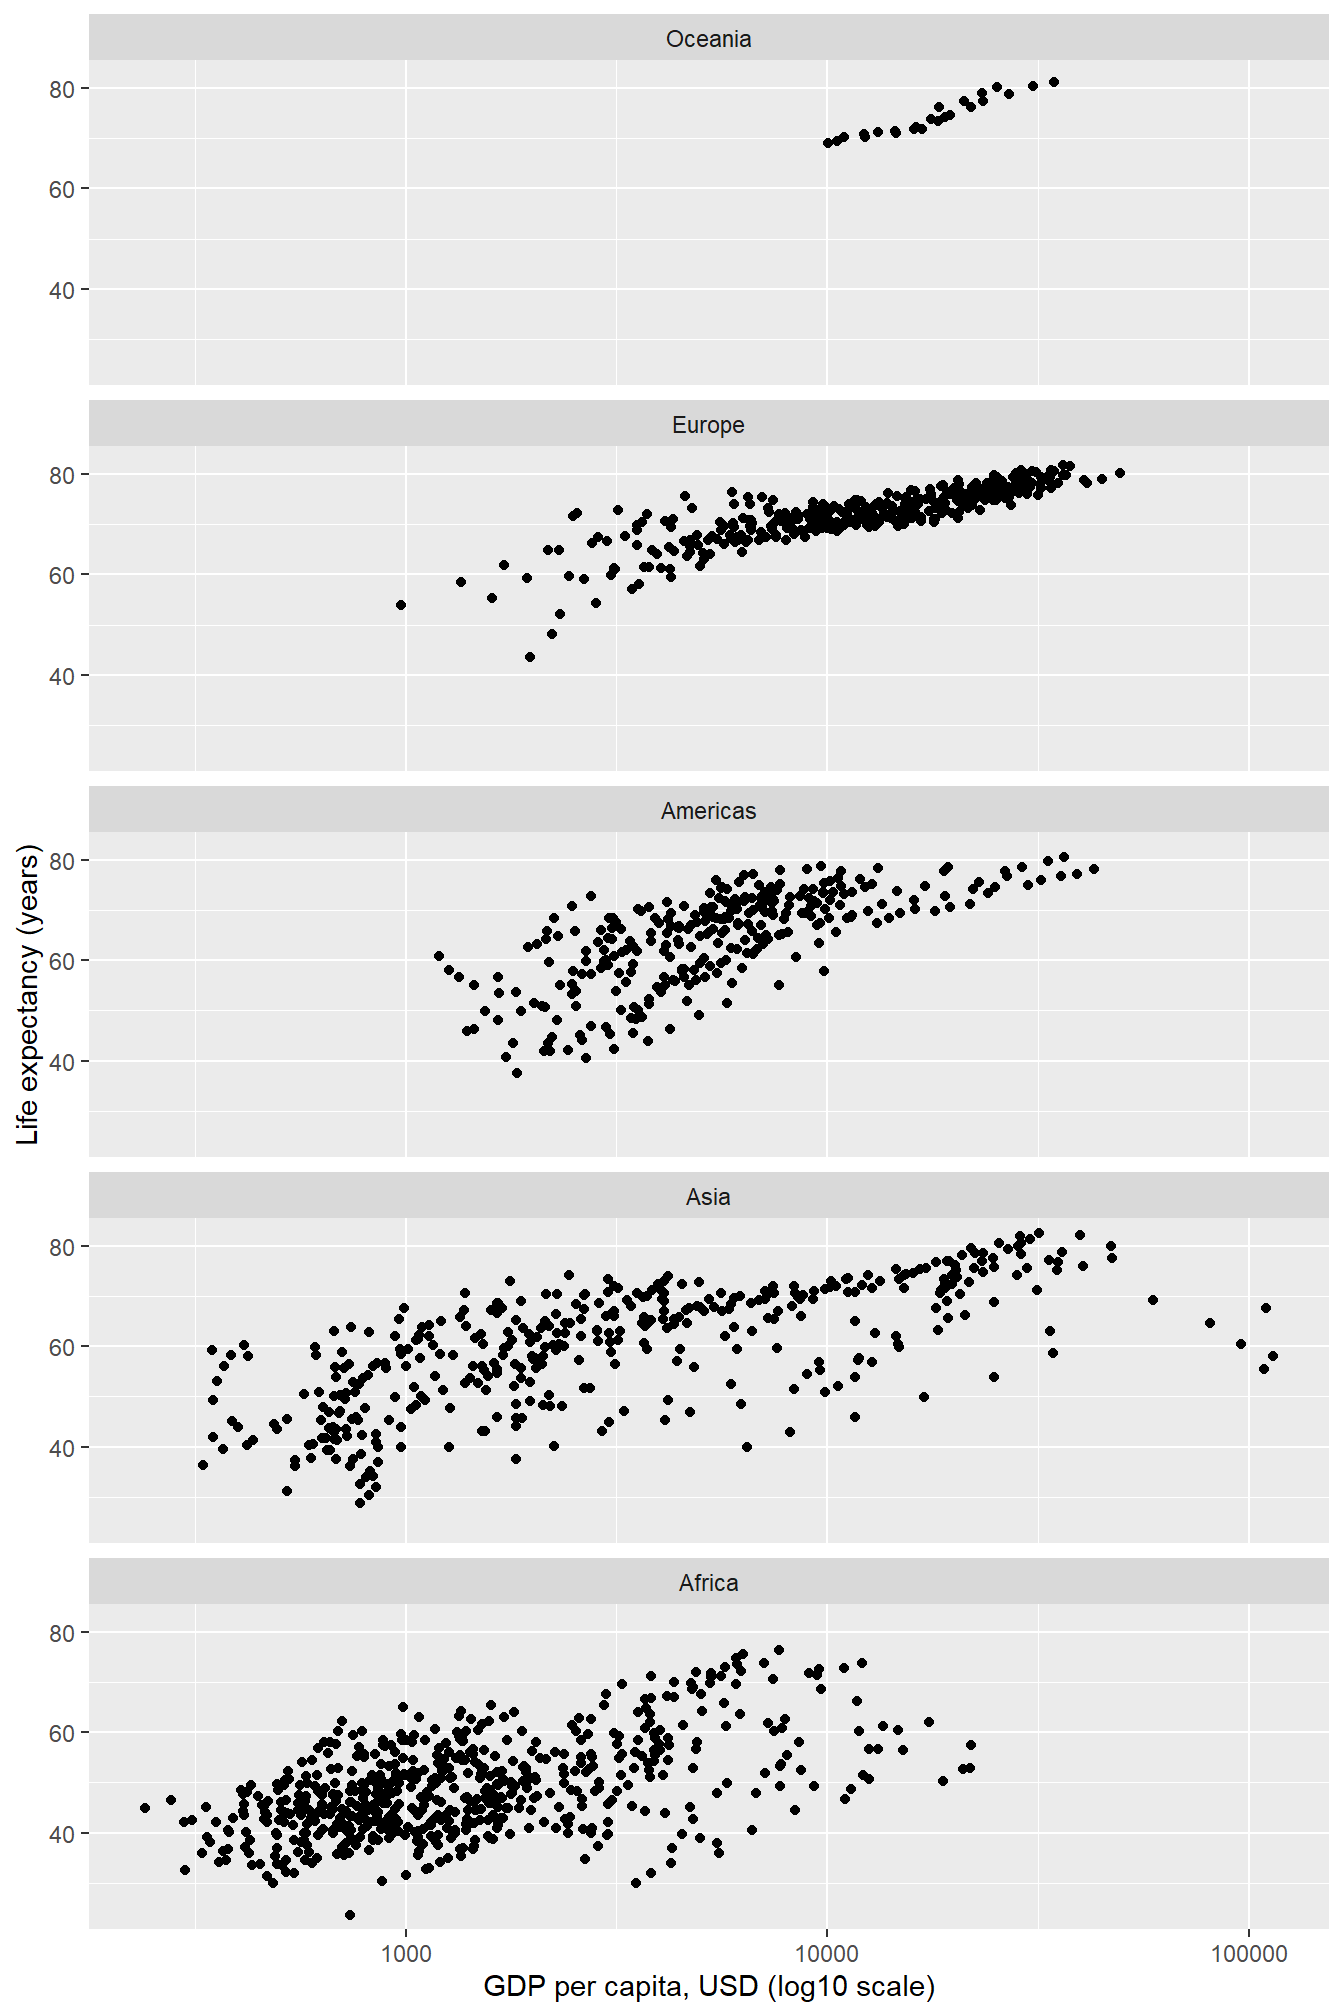
\includegraphics[width=0.8\linewidth]{2021-ASEE-Workshop_files/figure-latex/unnamed-chunk-85-1}

\hypertarget{exercise-6}{%
\subsection{Exercise}\label{exercise-6}}

\begin{itemize}
\tightlist
\item
  Continue using the \texttt{stickiness} data frame from the previous section.\\
\item
  Order the panels by the stickiness variable.
\item
  Order race/ethnicity/sex by the stickiness variable.
\item
  Check your work by comparing your result to the graph below.
\end{itemize}

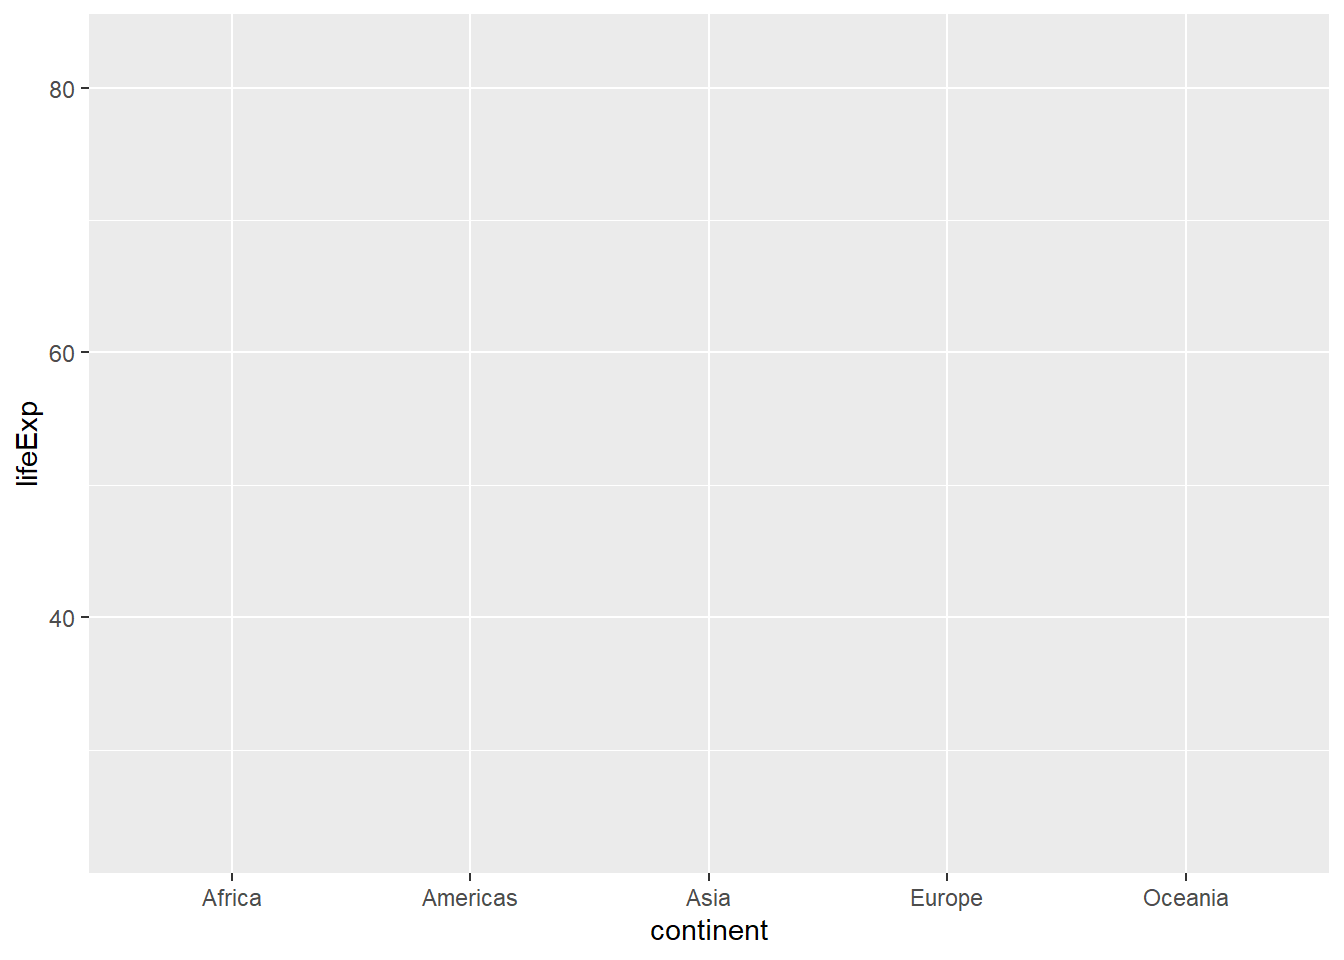
\includegraphics[width=0.8\linewidth]{2021-ASEE-Workshop_files/figure-latex/unnamed-chunk-86-1}

Help pages for more information:

\begin{itemize}
\tightlist
\item
  \href{https://www.rdocumentation.org/packages/stats/versions/3.6.2/topics/reorder.default}{reorder()}
\end{itemize}

\protect\hyperlink{start-with-R}{▲ top of page}

\hypertarget{data-basics}{%
\chapter{Data basics}\label{data-basics}}

\hypertarget{introduction-2}{%
\section{Introduction}\label{introduction-2}}

This tutorial is an introduction to \ldots{}

If you already have R experience, you might still want to browse this section in case you find something new.

\protect\hyperlink{prerequisites}{Prerequisites} should be completed before proceeding. After that, the tutorial should take about an hour.

Create a new script for this tutorial.

\begin{itemize}
\tightlist
\item
  See \protect\hyperlink{open-an-r-script}{Open an R script} if you need a refresher on creating, saving, and running an R script.
\item
  At the top of the script add a minimal header and install and load the packages indicated.
\end{itemize}

\begin{Shaded}
\begin{Highlighting}[]
\CommentTok{\# Data basics }
\CommentTok{\# name }
\CommentTok{\# date }

\FunctionTok{library}\NormalTok{(}\StringTok{"midfieldr"}\NormalTok{)}
\FunctionTok{library}\NormalTok{(}\StringTok{"data.table"}\NormalTok{)}
\FunctionTok{library}\NormalTok{(}\StringTok{"ggplot2"}\NormalTok{)}
\FunctionTok{library}\NormalTok{(}\StringTok{"gapminder"}\NormalTok{)}

\CommentTok{\# Optional code to control data.table printing}
\FunctionTok{options}\NormalTok{(}
  \AttributeTok{datatable.print.nrows =} \DecValTok{10}\NormalTok{,}
  \AttributeTok{datatable.print.topn =} \DecValTok{5}\NormalTok{,}
  \AttributeTok{datatable.print.class =} \ConstantTok{TRUE}
\NormalTok{)}
\end{Highlighting}
\end{Shaded}

If you get an error like this one after running the script,

\begin{verbatim}
    Error in library("gapminder") : there is no package called 'gapminder'
\end{verbatim}

then the package needs to be installed. If you need a refresher on installing packages, see \protect\hyperlink{install-cran-packages}{Install CRAN packages}. Once the missing package is installed, you can rerun the script.

Guidelines

\begin{itemize}
\tightlist
\item
  As you work through the tutorial, type a line or chunk of code then \emph{File \textgreater{} Save} and run the script.\\
\item
  Confirm that your result matches the tutorial result.\\
\item
  \textbf{Your turn} exercises give you chance to devise your own examples and check them out. You learn by doing (but you knew that already)!
\end{itemize}

\protect\hyperlink{start-with-R}{▲ top of page}

\hypertarget{display-design}{%
\chapter{Designing effective displays}\label{display-design}}

\hypertarget{stuff}{%
\section{Stuff}\label{stuff}}

\hypertarget{more-stuff}{%
\section{More stuff}\label{more-stuff}}

\protect\hyperlink{display-design}{▲ top of page}

  \bibliography{book.bib,packages.bib,references.bib}

\end{document}
